\documentclass[12pt,letterpaper]{book}
\usepackage[utf8]{inputenc}
\usepackage[T1]{fontenc}
\usepackage[spanish,es-tabla,es-nodecimaldot]{babel}

% Geometría del documento
\usepackage[left=3cm,top=3cm,right=3cm,,bottom=3cm]{geometry}
% Fuente Times New Roman
\usepackage{tgtermes}

\usepackage{amsmath}
\usepackage{amsfonts}
\usepackage{amssymb}
\usepackage{graphicx}
\usepackage{subfig}
\usepackage{wasysym}
\usepackage{lscape}
\usepackage{tabularx}
\usepackage{float}
\usepackage{booktabs}
\usepackage{setspace} %por si el titulo es mas largo y el interlineado
\usepackage{pdfpages}

\usepackage[colorlinks=true, linkcolor=black,
citecolor=black, urlcolor=black,hidelinks]{hyperref}
\usepackage[ruled,vlined]{algorithm2e}

% Texto Justificado
\usepackage[justification=centering]{caption}

% Reducimos el espacio debajo de las figuras
\captionsetup{belowskip=0pt}

% Interlineado 1.5
\renewcommand{\baselinestretch}{1.5}

% Citas en formato APA
\usepackage{csquotes}
\usepackage[backend=biber,natbib,url=false,doi=false,style=apa,maxcitenames=5]{biblatex}

% Cuando el idioma es otro "et al." cambia, con este comando se fuerza a si o si usar "et al."
\DefineBibliographyStrings{spanish}{%
  andothers = {et\addabbrvspace al\adddot}
}
\addbibresource{capitulos/biblio.bib}

% Eliminar la palabra "Capítulo" y forzar que sea del mismo tamaño que el resto del texto
\usepackage{titlesec}
%\titleformat{\chapter}
%  {\normalsize\bfseries}{\thechapter.}{0.5em}{}
%  \titlespacing*{\chapter}{0pt}{14pt}{14pt}
\newcommand{\negspacechap}{\titleformat{\chapter}		% nuevo comando eliminar espacio previo
	{\normalsize\bfseries}{\thechapter.}{0.5em}{}
	\titlespacing*{\chapter}{0pt}{-14pt}{2mm}}
\newcommand{\pospacechap}{\titleformat{\chapter}		% mantener el espacio reacomodar tamaño
	{\normalsize\bfseries}{\thechapter.}{0.5em}{}
	\titlespacing*{\chapter}{0pt}{14pt}{2mm}}

\newcommand{\negspacesec}{\titleformat{\section}		
	{\normalsize\bfseries}{\thesection.}{0.5em}{}
	\titlespacing*{\section}{0pt}{-14pt}{2mm}}
\newcommand{\pospacesec}{\titleformat{\section}		
	{\normalsize\bfseries}{\thesection.}{0.5em}{}
	\titlespacing*{\section}{0pt}{14pt}{2mm}}

\titleformat{\subsection}		
  {\normalsize\bfseries}{\thesubsection.}{0.5em}{}
  \titlespacing*{\subsection}{0pt}{2mm}{2mm}

% Cambiamos el tamaño de las secciones
\titleformat{\section}
  {\normalfont\normalsize\bfseries}{\thesection.}{0.5em}{}
\titleformat{\subsection}
  {\normalfont\normalsize\bfseries}{\thesubsection.}{0.5em}{}

% Elimina la cabecera de secciones y fuerza la numeración abajo
\usepackage{fancyhdr}
\fancyhf{}
\renewcommand\headrulewidth{0pt}
% Numeración a la derecha
\fancyfoot[R]{\thepage}
% Fuerza la numeración de páginas de capítulos a la derecha
\pagestyle{fancy}
\fancypagestyle{plain}{
    \renewcommand{\headrulewidth}{0pt}
    \fancyhf{}
    \fancyfoot[R]{\thepage}
}

% Elimina el indentado en la tabla de contenidos para subsecciones
\usepackage[subfigure]{tocloft}
\setlength{\cftsecindent}{1em}
\setlength{\cftsubsecindent}{1em}
\setlength{\cftsubsubsecindent}{1em}

% Considera 4 niveles de profundidad para el índice
\usepackage{enumitem}
\setcounter{tocdepth}{3}  % Originalmente 3
\setcounter{secnumdepth}{3}

% Para los algoritmos
\renewcommand*{\listalgorithmcfname}{Lista de Algoritmos}
\renewcommand*{\algorithmcfname}{Algoritmo}
\renewcommand*{\algorithmautorefname}{algoritmo}
\SetKwInput{KwData}{Requiere}

% Sobreescribir los capítulos para que empiecen seguidos sin saltos de páginas
\makeatletter
\patchcmd{\chapter}{\if@openright\cleardoublepage\else\clearpage\fi}{}{}{}
\makeatother

% Contar las figuras sin el capítulo
\usepackage{chngcntr}
\counterwithout{figure}{chapter}
\counterwithout{table}{chapter}

% Define el comando grad para insertar el símbolo de grados
\newcommand{\grad}{$^{\circ}$}

\usepackage{xcolor,colortbl}
\definecolor{none}{RGB}{0, 0, 0}
\definecolor{buildings}{RGB}{70, 70, 70}
\definecolor{fences}{RGB}{190, 153, 153}
\definecolor{other}{RGB}{72, 0, 90}
\definecolor{pedestrians}{RGB}{220, 20, 60}
\definecolor{poles}{RGB}{153, 153, 153}
\definecolor{roadlines}{RGB}{157, 234, 50}
\definecolor{roads}{RGB}{128, 64, 128}
\definecolor{sidewalks}{RGB}{244, 35, 232}
\definecolor{vegetation}{RGB}{107, 142, 35}
\definecolor{vehicles}{RGB}{0, 0, 255}
\definecolor{walls}{RGB}{102, 102, 156}
\definecolor{trafficsigns}{RGB}{220, 220, 0}

\usepackage{minted}
\usemintedstyle{tango}

\renewcommand{\cftbeforetoctitleskip}{-0.25in}
\renewcommand{\cfttoctitlefont}{\hspace{6.5cm}\large\bfseries}
\renewcommand{\cftaftertoctitleskip}{0.0\baselineskip}

%\renewcommand{\cftbeforeloftitleskip}{-1mm}
\renewcommand{\cftbeforeloftitleskip}{-0.25in}
\renewcommand{\cftloftitlefont}{\hspace{6.3cm}\large\bfseries}
\renewcommand{\cftafterloftitleskip}{0.0\baselineskip}

%\renewcommand{\cftbeforelottitleskip}{-0.01in}
\renewcommand{\cftbeforelottitleskip}{-0.25in}
\renewcommand{\cftlottitlefont}{\hspace{6.3cm}\large\bfseries}
\renewcommand{\cftafterlottitleskip}{0.0\baselineskip}

\begin{document}
	\frontmatter % numeros romanos
	\begin{titlepage} %este titlepage sirve para poder realizar el titulo de una pagina, la caratula de un libro y no se enumere esta.
	\begin{center}
		\begin{spacing}{1.8}
			{\large \textbf{UNIVERSIDAD MAYOR DE SAN ANDRÉS}}\\
			{\large \textbf{FACULTAD DE CIENCIAS PURAS Y NATURALES}}\\
			{\large \textbf{CARRERA DE INFORMÁTICA}}
		\end{spacing}
		\vspace{8mm}
		
		
\includegraphics[scale=0.11]{imagenes/logo-umsa.png}
		\vspace{6mm}
		
		\begin{spacing}{1.5}
			{\large \textbf{TESIS DE GRADO}}
		\end{spacing}
		\vspace{6mm}
		
		\begin{spacing}{1}
			{\large \textbf{MODELO DE CONDUCCIÓN AUTÓNOMA BASADO EN APRENDIZAJE PROFUNDO Y ALGORITMOS DE VISIÓN COMPUTACIONAL}}
		\end{spacing}
		\vspace{6mm}
		
		\begin{spacing}{1.3}
			{\textsc{PARA OPTAR AL TÍTULO DE LICENCIATURA EN INFORMÁTICA}}\\
			{\textsc{MENCIÓN: CIENCIAS DE LA COMPUTACIÓN}}
		\end{spacing}
		\vspace{6mm}
		
		\begin{spacing}{1.3}
			\begin{tabular}{rl}
				\textbf{POSTULANTE} & RAFAEL VILLCA POGGIAN\\
				\textbf{TUTOR METODOLÓGICO:} & M.Sc. ALDO VALDEZ ALVARADO\\
				\textbf{ASESOR:} & Lic. BRIGIDA ALEXANDRA CARVAJAL BLANCO \\
			\end{tabular}
		\end{spacing}
		\vspace{6mm}
		
		\begin{spacing}{1.3}
			\textbf{LA PAZ - BOLIVIA}\\
			\textbf{2021}
		\end{spacing}
		
	\end{center}
	
	%\begin{flushleft}
	%\section*{Personal Investigador}
	%\end{flushleft}
	
	%\vspace{4cm}
	%\rule{40mm}{0.3mm}
	
\end{titlepage}
	
\includepdf[page={2}]{T-3395}
%	Hola

	\setcounter{page}{3}
	\section*{DEDICATORIA}
\addcontentsline{toc}{section}{DEDICATORIA}
\vfill
\hfill\begin{minipage}{\dimexpr\textwidth-9cm}
Dedico la presente tesis a mi familia por todo el apoyo, amor y paciencia durante todos estos años de estudio.
\end{minipage}

\newpage
\section*{\hspace{5.5cm}AGRADECIMIENTOS}
\addcontentsline{toc}{section}{AGRADECIMIENTOS}

\begin{center}
	A mi familia por el apoyo durante todos los años cursando la carrera.\\
	\vspace{0.8cm}
	A mi tutor M.Sc. Aldo Valdez Alvarado por la guía durante el desarrollo de la presente tesis, y a mi asesora Lic. Brigida Carvajal Blanco por los consejos, sugerencias y apoyo.
\end{center}

\newpage
\section*{\hspace{6.4cm}RESUMEN}
\addcontentsline{toc}{section}{RESUMEN}
La creciente popularidad de vehículos de distintas marcas con funcionalidades autónomas, ocasionó la creación de simuladores y conjuntos de datos para el entrenamiento de modelos de conducción mediante técnicas de visión artificial y aprendizaje profundo.

El problema a abordar en las soluciones que se desarrollan es crear implementaciones eficientes para realizar inferencias rápidas y reaccionar a las distintas situaciones ambientales mediante cámaras.

Se propone un modelo compuesto por redes neuronales y algoritmos de visión computacional que se complementen, y así obtener una conducción autónoma básica y eficiente computacionalmente.\\

\noindent Palabras clave: Aprendizaje profundo, Visión computacional, Redes neuronales, Carla simulator

\newpage
\section*{\hspace{6.4cm}ABSTRACT}
\addcontentsline{toc}{section}{ABSTRACT}
The increasing popularity of different car manufacturers with autonomous features, made possible the creation of simulators and data sets to train self driving models using Computer Vision techniques and Deep Learning.

The main focus of these solutions is to develop efficient implementations to perform fast inference and react to different environmental situations through cameras.

In this work a model composed of deep neural networks and computer vision algorithms which work together is proposed, in order to obtain an efficient and basic self driving capability\\

\noindent Keywords: Deep learning, Computer vision, Neural networks, Carla simulator
	
	\tableofcontents
	\addcontentsline{toc}{section}{ÍNDICE}
	\newpage
	\listoffigures
	\addcontentsline{toc}{section}{ÍNDICE DE FIGURAS}
	\newpage
	\listoftables
	\addcontentsline{toc}{section}{ÍNDICE DE TABLAS}
	
	% Elimina página en blanco luego de la lista de tablas
	\let\cleardoublepage\clearpage
	
	\mainmatter %numeros arabicos.
    \setcounter{page}{1}
    \raggedbottom
	\negspacechap
\chapter{MARCO REFERENCIAL}
%\chapter[Marco Referencial]{MARCO REFERENCIAL}
	\negspacesec
    \section{INTRODUCCIÓN}
%\section[Introducción]{INTRODUCCIÓN}
Los vehículos autónomos son algo común en el imaginario colectivo, esto debido a sus apariciones en la ciencia ficción y a las noticias de que empresas como Waymo, Uber y muchas más están trabajando para lograr la tan deseada autonomía completa.

Los modelos de Machine Learning usados en la actualidad fueron desarrollados muchas décadas atrás, estos requerían pre procesar demasiado la información de conjuntos de datos pequeños, sin embargo gracias a los avances en la transmisión de la información y al acceso a datos masivos que antes no eran posibles de almacenar, estos requisitos fueron decreciendo mientras más datos de entrenamiento se tenían disponibles, es así como se da un resurgimiento en el interés por los modelos probabilísticos, superando estos a los basados en reglas, utilizados comúnmente hasta los años 90. \citep{Goodfellow-et-al-2016}
% (Goodfellow, Bengio, \& Courville, 2015)

En el ámbito de la visión computacional, los primeros modelos eran capaces de detectar objetos simples en imágenes muy pequeñas \citep{Rumelhart_Hinton_Williams_1986}. Por contraparte los modelos modernos basados en Redes Neuronales Convolucionales, son capaces de detectar por lo menos 1000 categorías distintas con una exactitud muy superior a los métodos clásicos siempre y cuando la cantidad de datos sea suficiente. \citep{alexnet}
% (Krizhevsky, Sutskever, \& Hinton, 2012)\\

Aprovechando los avances de la visión computacional y la mejora de mejores sensores, los sistemas de conducción autónoma refinaron su capacidad de percepción, etapa clave para la toma de decisiones, mediante el uso de las Redes Neuronales para la detección, segmentación y clasificación de objetos en las carreteras, con los más avanzados como el autopilot de Tesla detectando situaciones adversas basado en acciones de otros vehículos en el camino a tiempo real. \citep{karpathy-scaledml}
% (Karpathy, 2020)

En el presente trabajo se propone un modelo compuesto por redes neuronales convolucionales y algoritmos de visión artificial para resolver las tareas básicas requeridas para la percepción y control de un vehículo autónomo.
\newpage  % Corregir la intro
    \section{ANTECEDENTES}
%\section[Antecedentes]{ANTECEDENTES}
A continuación se revisa la evolución de los métodos de visión computacional aplicados en la conducción autónoma y los sistemas resultantes aplicados a esta tarea.
\subsection{ESTADO DEL ARTE}
%\subsection[Estado del Arte]{ESTADO DEL ARTE}
Se revisa el desarrollo de las tecnologías a utilizar desde su creación hasta el momento.

\subsubsection{DETECCIÓN DE OBJETOS}
%\subsubsection[Detección de Objetos]{DETECCIÓN DE OBJETOS}
\paragraph{1963 PERCEPCIÓN DE SÓLIDOS TRIDIMENSIONALES}
Lawrence Roberts desarrollo un algoritmo para detectar figuras sólidas simples en imágenes, extraer su estructura característica en forma de líneas para poder aplicarles transformaciones de perspectiva en un espacio 3D. \citep{Roberts_1963}
% (Robert, 1963)

\begin{figure}[H]
    \centering
    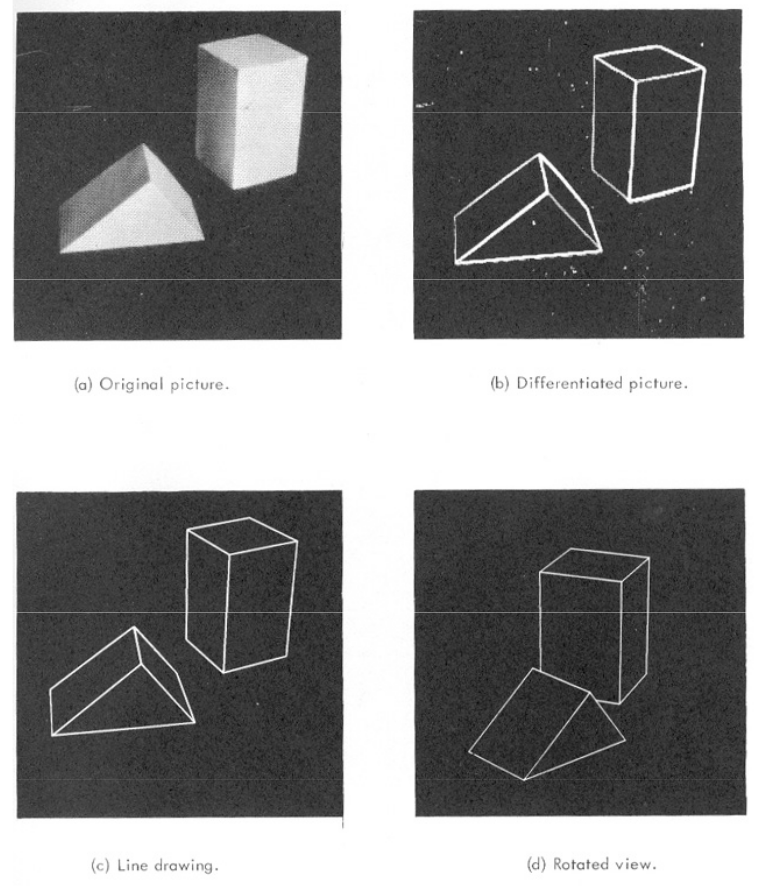
\includegraphics[scale=0.25]{imagenes/machine-perception-of-three-dimensional-solids}
    \caption[Contornos de objetos]{Detección de contornos de objetos\\Fuente: \citep{Roberts_1963}}
\end{figure}
% \vspace{-6mm}
% \begin{center}
%     Fuente: Artículo original
% \end{center}
\paragraph{2001 HAAR FEATURES}
Paul Viola y Michael Jones desarrollaron el algoritmo Viola-Jones, el cual significó un cambio radical en los métodos de detección de objetos, extrayendo características primitivas con clasificadores débiles uno detrás del otro, y aplicando la técnica de la imagen integral, fueron capaces de detectar distintos tipos de objetos en imágenes de manera óptima, entrenando el método sobre un conjunto pequeño de imágenes. Este método se usa hasta hoy en día en cámaras celulares para la detección de rostros. \citep{haar-cascade}
% (Viola \& Jones, 2001)

\begin{figure}[H]
    \centering
    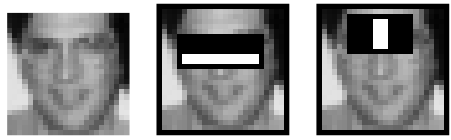
\includegraphics[scale=0.4]{imagenes/haar}
    \caption[Características HAAR]{Características Haar buscando patrones en la imágen\\Fuente: \citep{haar-cascade}}
\end{figure}
% \vspace{-6mm}
% \begin{center}
%     Fuente: Artículo original
% \end{center}
\paragraph{2005 HISTOGRAMAS DE GRADIENTES ORIENTADOS}
En 1986 Robert K. McConnell describe un descriptor de características que sería conocido como HOG o histograma de gradientes orientados, en 2005 sería aplicado a la detección de personas, rivalizando con el método de características Haar. \citep{hog-paper}
% (Dalal \& Triggs, 2005) 

\begin{figure}[H]
    \centering
    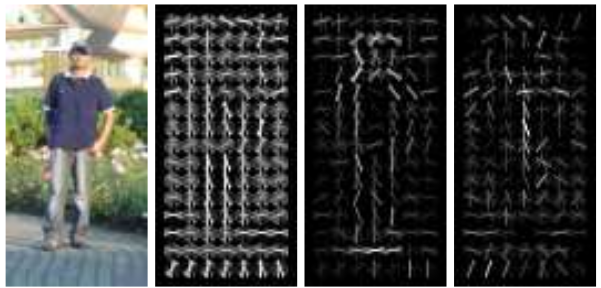
\includegraphics[scale=0.4]{imagenes/hog}
    \caption[Vectores direccionales del HOG]{Vectores direccionales del HOG\\Fuente: \citep{hog-paper}}
\end{figure}
% \vspace{-6mm}
% \begin{center}
%     Fuente: Artículo original
% \end{center}
\paragraph{2016 YOLO}
La búsqueda de métodos que aceleren el proceso de ventanas deslizantes para localizar objetos, llevó a buscar alternativas que realicen todo el proceso en una sola pasada del método, así nace You Only Look Once, una arquitectura de red neuronal convolucional que barre la imágen en grillas definidas buscando la existencia del centro de un objeto y realizando una supresión de no máximo para eliminar ocurrencias repetidas, siendo uno de los métodos más efectivos en la detección de objetos. \citep{Redmon2016YouOL}
% (Redmon, Divvala, Girshick, \& Farhadi)
% \newpage
\begin{figure}[H]
    \centering
%    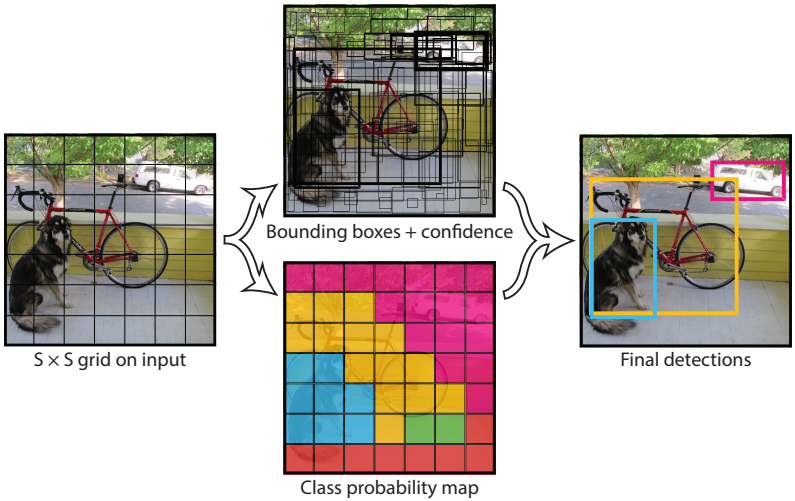
\includegraphics[scale=0.4]{imagenes/yolo}
	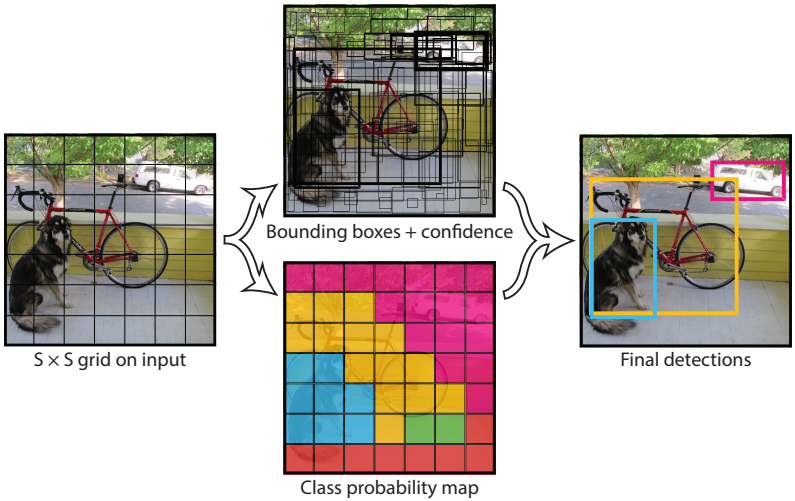
\includegraphics[scale=0.5]{imagenes/yolo}
    \caption[Flujo predicción YOLO]{Flujo predicción YOLO\\Fuente: \citep{Redmon2016YouOL}}
\end{figure}
% \vspace{-6mm}
% \begin{center}
%     Fuente: Artículo original
% \end{center}
\paragraph{2016 SSD}
Con una arquitectura distinta aplicando la misma idea de la partición de la imágen en una grilla, se propone el método Single Shot MultiBox Detector, el cual es menos preciso en la detección de objetos que su contraparte YOLO, pero más rápido y capaz de detectar objetos más pequeños en la imágen. \citep{liu-ssd}
% (Liu et al, 2016)

\begin{figure}[H]
    \centering
%    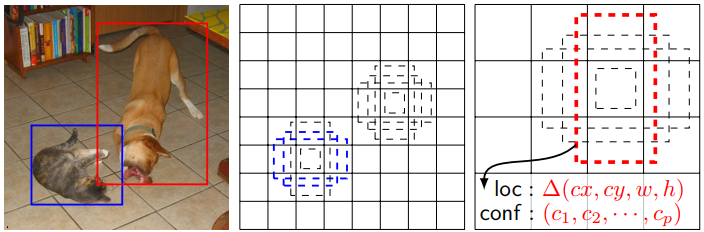
\includegraphics[scale=0.4]{imagenes/ssd}
	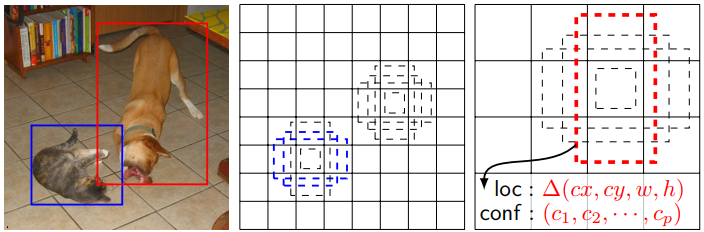
\includegraphics[scale=0.5]{imagenes/ssd}
    \caption[Partición y recuadros de detección SSD]{Partición y recuadros de detección SSD\\Fuente: \citep{liu-ssd}}
\end{figure}

% \vspace{-6mm}
% \begin{center}
%     Fuente: Artículo original
% \end{center}
\paragraph{2020 RETINANET}
Buscando solucionar el problema de la detección de objetos pequeños y en gran cantidad en un entorno denso, mediante modificaciones en la función de costo del clasificador, nace la llamada Retinanet. \citep{retinanet}

\subsubsection{SEGMENTACIÓN SEMÁNTICA}
%\subsubsection[Segmentación Semántica]{SEGMENTACIÓN SEMÁNTICA}

\paragraph{SEGMENTACIÓN POR COLOR Y ESCALA DE GRISES}
Entre los primeros métodos de segmentación semántica están los de segmentación por burbujas de color en espacios de color alternativos al RGB, de forma que toda un área de un color específico con alguna variación permitida era enmascarada como un objeto en la imágen.

\paragraph{2004 CAMPOS ALEATORIOS CONDICIONALES MULTIESCALA}
La idea de los campos aleatorios condicionales, (MCRF abreviado en inglés) nació para etiquetar y segmentar secuencias de textos, pero fue modificada para lograr segmentar elementos de una imagen, modelando la relación espacial entre los píxeles con una probabilidad condicional que pertenezca a alguna clase dada la clase de los píxeles vecinos, aplicando un campo estocástico bidimensional (generalización de un proceso estocástico). \citep{segmentation-crf}

\begin{figure}[H]
    \centering
%    \subfloat[imágen original]{{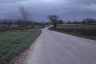
\includegraphics[width=5cm]{imagenes/mcrf1} }}%
    \subfloat[imágen original]{{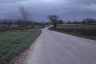
\includegraphics[width=6cm]{imagenes/mcrf1} }}%
    \qquad
    \subfloat[segmentación con MCRF]{{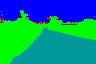
\includegraphics[width=6cm]{imagenes/mcrf2} }}%
    \caption[Segmentación de carretera por MCRF]{Segmentación de carretera por MCRF\\Fuente: \citep{segmentation-crf}}
\end{figure}

\paragraph{2015 U-NET}
Inicialmente pensada para aplicaciones médicas, esta arquitectura de Red Neuronal Convolucional probó ser efectiva en muchas tareas se segmentación, extendiendo la idea de un auto encoder con saltos entre capas, la topología de las conexiones de la red forman una U, de donde proviene su nombre. \citep{u-net}

\begin{figure}[H]
    \centering
    \subfloat[imágen original]{{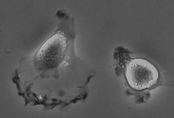
\includegraphics[width=5cm]{imagenes/u-net-1} }}%
    \qquad
    \subfloat[segmentación con U-Net]{{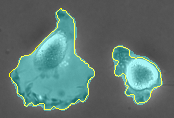
\includegraphics[width=5cm]{imagenes/u-net-2} }}%
    \caption[Segmentación de una célula del dataset PhC-U373]{Segmentación de una célula del dataset PhC-U373\\Fuente: \citep{u-net}}%
    \label{unet}%
\end{figure}
% \vspace{-6mm}
% \begin{center}
%     Fuente: Artículo U-Net
% \end{center}

% \newpage

\paragraph{2017 MASK-RCNN}
Siguiendo la propuesta de una red de dos etapas, dividiendo la tarea en dos más sencillas, esta arquitectura primero propone regiones de interés en base a las cuales hace dos tipos de inferencia, una regresión de los puntos delimitando un rectángulo que encierra a cada objeto, y una máscara binaria para cada clase a segmentar. \citep{mask-rcnn} Junto a la U-Net son los dos métodos más usados en la actualidad, incluido en el dominio de vehículos autónomos.

\begin{figure}[H]
    \centering
    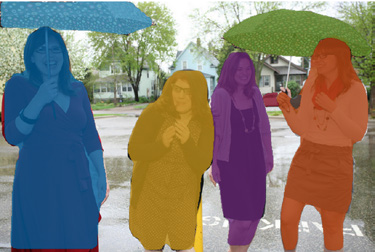
\includegraphics[scale=0.5]{imagenes/maskrcnn}
    \caption[Segmentación semántica de distintas clases]{Segmentación semántica de distintas clases\\Fuente: \citep{mask-rcnn}}
\end{figure}
% \vspace{-6mm}
% \begin{center}
%     Fuente: Artículo original Mask-RCNN
% \end{center}
\subsubsection{SISTEMAS DE CONDUCCIÓN AUTÓNOMA}
%\subsubsection[Sistemas de Conducción Autónoma]{SISTEMAS DE CONDUCCIÓN AUTÓNOMA}

\paragraph{2004 DAVE}
Uno de los primeros intentos de programar un sistema de conducción autónoma fue propuesto por un equipo en el que se encontraba Yann LeCun, uno de los precursores en el uso de las redes convolucionales. En este proyecto se usaban dos cámaras, se entrenó una red en imágenes capturadas en un vehículo a control remoto, y se realizaba una predicción del nivel de aceleración y ángulo de rotación para cada fotograma capturado. \citep{LeCun:04-dave}

\begin{figure}[H]
    \centering
    \subfloat[Vehículo DAVE]{{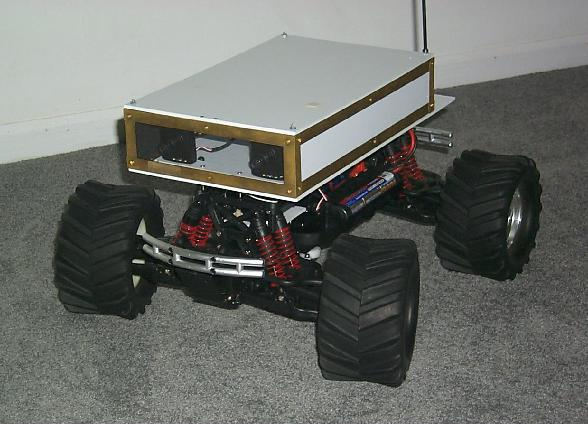
\includegraphics[width=4cm]{imagenes/dave-1} }}%
    \qquad
    \subfloat[Predicción del ángulo de rotación]{{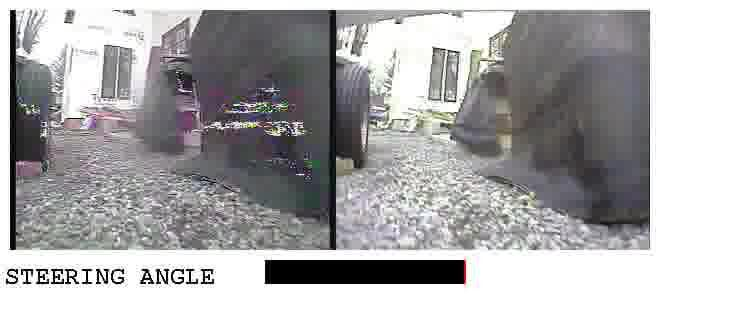
\includegraphics[width=6cm]{imagenes/dave-2} }}%
    \caption[DAVE]{Fuente: Reporte \citep{LeCun:04-dave}}%
    \label{dave}%
\end{figure}

\paragraph{2004 DARPA GRAND CHALLENGE}
La agencia de investigación en proyectos de defensa avanzados o DARPA abreviado en inglés, organizó una comptenecia en el desierto Mojave, con una pista preparada en un terreno arenoso. Los vehículos concursantes podían usar distintos tipos de sensores como cámaras, radar, lidar y GPS. \citep{hooper_2004}

\paragraph{2010 GOOGLE}
Después de muchos tests con asistencia humana y sin llamar la atención, se hacen públicos los experimentos de Google en la vía publica con vehículos equipados con sensores y un sistema de conducción autónoma. Este sistema iría evolucionando hasta la actualidad, cuando después de un cambio de nombre del proyecto, ahora bajo la marca Waymo, Ya realizan trayectos totalmente autónomos. \citep{markoff_2010}

\paragraph{2015 TESLA}
Tesla inició su programa de conducción autónoma oficialmente el año 2015, con un actualización de software para los Tesla Model S equipados con el Hardware necesario para el funcionamiento de su Autopilot. \citep{nelson_2015} Posteriormente después de varias actualizaciones de software, y una de hardware, los distintos vehículos sucesivos de Tesla recopilarían los datos necesarios de los trayectos realizados por los usuarios para mejorar la reacción de este sistema. \citep{karpathy-scaledml}

\subsection{TRABAJOS SIMILARES}
%\subsection[Trabajos Similares]{TRABAJOS SIMILARES}

\begin{itemize}[nosep]
    \item[] \textbf{Título:} Aprendizaje fin a fin para la conducción autónoma de vehículos domésticos usando visión artificial y redes neuronales convolucionales.
    \item[] \textbf{Autor:} Jose Eduardo Laruta Espejo
    \item[] \textbf{Año:} 2018
    \item[] \textbf{Institución:} Universidad Mayor de San Andrés
    \item[] Esta tesis plantea implementar un sistema fin a fin embedido, equipado con una raspberry pi, que recibía fotogramas de una pista para carreras y debía predecir con una sola red neuronal, el ángulo de rotación de los servomotores y la aceleración para cada fotograma.
\end{itemize}

\begin{itemize}[nosep]
    \item[] \textbf{Título:} Deep Vision Pipeline for Self-Driving Cars Based on Machine Learning Methods.
    \item[] \textbf{Autor:} Mohammed Nabeel Ahmed
    \item[] \textbf{Año:} 2017
    \item[] \textbf{Institución:} Ryerson University
    \item[] Este trabajo propone un flujo de datos para procesar la información en base a cámaras, mediante detección de las líneas de carreteras, clasificación de signos de tráfico y vehículos para realizar control del vehículo usando la predicción de estos.
\end{itemize}

\begin{itemize}[nosep]
    \item[] \textbf{Título:} Modelamiento Semántico del Entorno para la Conducción Autónoma de un Vehículo Terrestre
    \item[] \textbf{Autor:} Fernando Javier Bernuy Bahamóndez
    \item[] \textbf{Año:} 2017
    \item[] \textbf{Institución:} Universidad de Chile
    \item[] La tesis doctoral, propone el uso de segmentación semántica para apoyar técnicas clásicas de visión computacional para la localización espacial de un vehículo en un entorno urbano, logrando ubicarse en posiciones del terreno, estimar su orientación y lugar del recorrido planeado.
\end{itemize}
    
    \pospacesec
    \section{PLANTEAMIENTO DEL PROBLEMA}
%\section[Plantemaiento del Problema]{PLANTEAMIENTO DEL PROBLEMA}
Si bien la idea de construir vehículos autónomos no es nueva, es en esta época donde finalmente se está logrando salir de etapas prototipo, a incluir estos sistemas en vehículos de venta masiva, por parte de distintos fabricantes, de entre los cuales uno de los más reconocidos es Tesla Motors, que a diferencia de las alternativas propuestas por Google y Uber, proponen un sistema sin el uso de sensores costosos y poco estéticos para un vehículo comercial como un LIDAR \citep{granath_2020}, basandose sólamente en sensores de proximidad, radar, GPS y múltiples cámaras, diseñando y entrenando sus modelos de aprendizaje profundo como arquitecturas de redes neuronales y aprendizaje reforzado, con los datos masivos recopilados de los vehículos vendidos que circulan día a día \citep{karpathy-scaledml}, buscando que sus vehículos sean capaces de conducirse en todo tipo de situaciones climáticas y de iluminación, ya que los modelos de aprendizaje profundo superan a los algoritmos de visión computacional en estas situaciones \citep{Goodfellow-et-al-2016}, si se tiene la gran cantidad de datos para entrenarlos correctamente. \citep{alexnet}
% , usando estas últimas para las tareas de percepción y toma de decisiones inmediatas aplicando distintos algoritmos de visión computacional clásica y moderna con Deep Learning.

Un coche que se conduzca solo, respetando todas las leyes de tránsito, con tiempos de reacción instantáneos y sin problemas humanos como el cansancio, en un ecosistema compuesto en su totalidad por vehículos autónomos, reduciría el riesgo de accidentes de tránsito. Existe un historial de accidentes en los que están envueltos autos autónomos, de estos, la mayoría fueron causados por otros conductores humanos que al no respetar las reglas de tránsito impactaron de alguna manera con el vehículo autónomo \citep{wikipedia_2020}. Por esta razón y debido a la forma de vida acelerada en la sociedad actual, automatizaciones que ahorren tiempo en alguna actividad, son productos atractivos en los que se invierte para su investigación, existiendo en el caso de los vehículos autónomos datasets como el Open Waymo dataset, el cual contiene 2TB de datos para que los concursantes implementen sistemas de conducción autónoma y compitan en distintos retos. \citep{waymo}
% Por esta razón y porque en estos tiempos dónde las personas están cada vez más ocupadas con sus obligaciones y actividades, cualquier tarea que sea considerada un gasto de tiempo y sea automatizable, siempre será un factor atractivo. Uno en el que las empresas automotrices están invirtiendo y debido a esto existe un gran interés científico por investigar métodos eficientes para llevarlo a cabo.

Aparte de aplicaciones en la movilidad doméstica, existen áreas de investigación en vehículos autónomos para competencias tanto a escala como con vehículos reales, y también se busca aplicar esta tecnología en situaciones de trabajo con maquinaria pesada que conlleva cierto riesgo en la operación de esta.

\subsection{PROBLEMA CENTRAL}
%\subsection[Problema Central]{PROBLEMA CENTRAL}
% ¿De qué manera se puede conseguir un nivel de autonomía básico en la conducción de un vehículo en pistas y carreteras usando solamente cámaras y algoritmos de visión computacional y modelos aprendizaje profundo?
%¿De qué manera conseguir un nivel de autonomía básico en la conducción de un vehículo en pistas y carreteras?
¿De qué manera conseguir un nivel básico de conducción autónoma en vías de doble sentido?

\subsection{PROBLEMAS SECUNDARIOS}
%\subsection[Problemas Secundarios]{PROBLEMAS SECUNDARIOS}
\begin{itemize}[nosep]
%    \item Los conjuntos de datos disponibles contienen información de distintos sensores y cámaras sin procesamiento previo, debido a esto los datos pesan demasiado y existe mucha variabilidad en la distribución de imágenes.
%    \item Para lograr una buena autonomía son necesarios componentes de hardware avanzados como un LIDAR que brindan una mejor percepción del espacio, esto ocasiona que el precio de los sistemas de conducción autónoma sea elevado, poco accesible a estos componentes y complejiza el problema de implementación.
%    \item Los algoritmos de visión computacional requieren poca capacidad de cómputo, pero sólo funcionan en condiciones ideales de imágenes para los que se programan, esto ocasiona problemas con cambios en el contenido, perspectiva e iluminación.
%    \item Los modelos de aprendizaje profundo generalizan bien pero un modelo de varias capas es más complejo de entrenar, hace necesario recopilar muchos datos y requiere mucho poder de cómputo.
%    \item Los sistemas basados en reglas de decisión predefinidas no logran extrapolar el conocimiento correctamente a situaciones para las que no se programe una reacción, lo que da lugar a problemas de generalización.
	\item Los conjuntos de datos disponibles contienen información de distintos sensores y cámaras sin procesamiento previo, debido a esto los datos pesan demasiado y no se tiene información organizada y etiquetada.
	
	\item Para lograr una buena autonomía son necesarios componentes de hardware avanzados como un LIDAR que brindan una mejor percepción del espacio, esto ocasiona que el precio de los sistemas de conducción autónoma sea elevado y poco accesible, además de complejizar el problema de implementación.
	
	\item Los modelos de aprendizaje profundo generalizan bien pero un modelo de varias capas es más complejo de entrenar, hace necesario recopilar muchos datos y requiere mucho poder de cómputo.
	
	\item Al entrenar modelos simples de aprendizaje profundo, las representaciones profundas pueden ser subóptimas, esto ocasiona problemas con cambios en el contenido, perspectiva e iluminación.
	
	\item Los algoritmos de visión computacional requieren poca capacidad de cómputo, pero sólo funcionan en condiciones ideales de imágenes para los que se programan, esto da lugar a problemas de generalización de las predicciones.
	
	\item Acceder a un vehículo autónomo para realizar pruebas de rendimiento de un modelo es una tarea complicada de lograr, esto hace costoso el desarrollo de la tecnología y la mejora de los modelos disponibles para esta tarea.
\end{itemize}
    
    \section{DEFINICIÓN DE OBJETIVOS}
%\section[Definición de Objetivos]{DEFINICIÓN DE OBJETIVOS}

\subsection{OBJETIVO GENERAL}
%\subsection[Objetivo General]{OBJETIVO GENERAL}
% Desarrollar un sistema de conducción autónoma mediante el uso de técnicas de visión computacional clásica y moderna.

% Desarrollar un flujo de entrenamiento e inferencia de algoritmos de visión computacional y modelos de aprendizaje profundo aplicados a las tareas necesarias para conseguir un nivel de autónoma básico en pistas y carreteras.

% Desarrollar un flujo que permita el entrenamiento de modelos de aprendizaje profundo que combinados con algoritmos de visión computacional logren una conducción autónoma básica en pistas y carreteras.
Plantear un modelo para la conducción autónoma que logre una autonomía básica en vías de doble sentido con separación física.

%3 y 5
\subsection{OBJETIVOS ESPECÍFICOS}
%\subsection[Objetivos Específicos]{OBJETIVOS ESPECÍFICOS}
\begin{itemize}[nosep]
%    \item Diseñar un componente de aumentación y preprocesamiento de datos para extraer la información útil de los datasets y fuentes de datos disponibles.
	\item Diseñar un componente de aumentación y preprocesamiento de datos para extraer y crear un dataset con el fin de resolver la tarea.
    % \item Reducir la complejidad de la implementación del flujo mediante el uso de sólamente cámaras.
    \item Reducir la complejidad de implementación del modelo mediante el uso de solamente una cámara.
    
%    \item Analizar y entrenar redes neuronales con una alta exactitud en las predicciones utilizando menos requisitos de cómputo.
    \item Modificar y entrenar redes neuronales con una alta exactitud en las predicciones utilizando menos requisitos de cómputo.
    
    \item Analizar las predicciones de los modelos entrenados para comprobar si las representaciones aprendidas son invariantes a los cambios de perspectiva, iluminación y objetos en la imagen.
    
%    \item Implementar un componente que combine la predicción de algoritmos de visión computacional y modelos de aprendizaje profundo para mejorar la generalización de predicciones.
	\item Combinar las salidas de algoritmos de visión computacional y modelos de aprendizaje profundo para mejorar la generalización de predicciones.
    
    \item Probar el rendimiento del modelo en una simulación, analizando casos de fallas y qué situaciones puede manejar correctamente.
\end{itemize}
    
    \section{HIPÓTESIS}
% El flujo permite el entrenamiento de modelos de aprendizaje profundo con altos porcentajes de exactitud, que en conjunto con algoritmos de visión computacional, logran una conducción autónoma básica en situaciones de carreteras y pistas de competencia.
%El uso de aprendizaje profundo y algoritmos de visión computacional, permiten plantear un modelo con el cual un vehículo logra la autonomía básica en caminos de doble vía
El modelo de conducción autónoma mediante el uso de aprendizaje profundo y algoritmos de visión computacional alcanza una autonomía de nivel 2 en vías de doble sentido con separación física.

\subsection{OPERACIONALIZACIÓN DE VARIABLES}

\begin{center}
	\footnotesize
    \begin{tabular}{|c|c|}
        \hline
        \textbf{Variable} & \textbf{Tipo} \\
        \hline
        Aprendizaje profundo y algoritmos de visión computacional & Independiente \\
        \hline
        Modelo de conducción autónoma & Interviniente\\
        \hline
    \end{tabular}\\
    \vspace{2mm}
    \textbf{Fuente:} Elaboración propia
\end{center}
    
    \section{JUSTIFICACIÓN}
%\section[Justificación]{JUSTIFICACIÓN}
    \subsection{JUSTIFICACIÓN ECONÓMICA}
%    \subsection[Justificación Económica]{JUSTIFICACIÓN ECONÓMICA}
    La implementación reduce los costos al implementar un sistema de conducción autónoma ya que procura utilizar solamente una cámara sin el apoyo de sensores extra, lo que reduce la complejidad de todo el flujo de modelos y datos, centrando todos los esfuerzos en la implementación y entrenamiento de los algoritmos y modelos necesarios para esta tarea.
    \subsection{JUSTIFICACIÓN SOCIAL}
%    \subsection[Justificación Social]{JUSTIFICACIÓN SOCIAL}
    El presente trabajo propone un paso para hacer más accesible la conducción autónoma en vehículos convencionales, haciendo más fácil la adaptación de los vehículos de empresas y particulares.
    \subsection{JUSTIFICACIÓN CIENTÍFICA}
%    \subsection[Justificación Científica]{JUSTIFICACIÓN CIENTÍFICA}
    La investigación emplea técnicas de preprocesamiento de datos, procesamiento de imágenes mediante algoritmos de visión computacional y arquitecturas de redes neuronales para predecir las acciones necesarias en la conducción autónoma a partir de los datos obtenidos por la cámara.
    
    \section{ALCANCES Y LÍMITES}
%\section[Alcances y Límites]{ALCANCES Y LÍMITES}
	\subsection{ALCANCES}
%	\subsection[Alcances]{ALCANCES}
		\begin{itemize}[nosep]
			\item Se define una red neuronal para predecir fin a fin la aceleración y dirección del vehículo dado un fotograma de la cámara.
			\item El modelo contiente un módulo de estimación de distancias para evitar colisiones.
			\item Se introduce un módulo de segmentación de objetos en la imagen.
			\item Se implementa un algoritmo para la detección de objetos en base a las predicciones de las redes neuronales.
			\item El modelo contempla un módulo de clasificación de color de semáforos.
		\end{itemize}
	\subsection{LÍMITES}
%	\subsection[Límites]{LÍMITES}
		\begin{itemize}[nosep]
			\item El modelo no empleará módulos que tengan como entrada otros sensores aparte de una cámara RGB.
			\item Las predicciones del modelo no serán capaces de permitir cambios de carriles o adelantamientos.
			\item Las calles sobre las que puede conducirse tienen un carril en cada dirección y están asfaltadas.
			\item El modelo no es capaz de predecir correctamente en situaciones de lluvia extrema.
			\item La generalización del modelo está limitada por la complejidad de las redes neuronales a favor de velocidad de cómputo.
		\end{itemize}

%    \subsection{ALCANCES}
%    \begin{itemize}[nosep]
%        \item El modelo permitirá procesar imágenes de tramos vehiculares para el entrenamiento de modelos.
%        \item El modelo definirá arquitecturas de redes neuronales y algoritmos de visión computacional para la detección de carriles y circulación dentro de estos.
%        \item El modelo permitirá entrenar redes neuronales para predecir la velocidad y la rotación de la dirección del vehículo dado un fotograma de la cámara.
%        \item El modelo permitirá entrenar detectores de señales de tránsito para la toma de decisiones en base a estas.
%        \item El modelo entrenará detectores de peatones y vehículos en el camino para evitar colisiones y accidentes.
%        \item El modelo se probará en un simulador para comprobar su rendimiento en situaciones de caminos y pistas.
%    \end{itemize}
%    \subsection{LÍMITES}
%    \begin{itemize}[nosep]
%        \item El modelo no empleará modelos que tengan como entrada otros sensores aparte de cámaras RGB.
%        \item El modelo con los modelos y algoritmos, busca una autonomía básica, por lo tanto no se conseguirá una autonomía total que funcione en todo tipo de condiciones.
%        \item El modelo implementará algoritmos que no serán capaces de tomar decisiones avanzadas como cambios de carriles o adelantamientos.
%    \end{itemize}
    
    \section{APORTES}%
%\section[Aportes]{APORTES}
	\subsection{PRÁCTICO}
%    \subsection[Práctico]{PRÁCTICO}
    En el presente trabajo se presentarán algoritmos de visión computacional los cuales se combinarán con las predicciones de redes neuronales convolucionales en un flujo que inicia por preprocesar la información para luego entrenar los componentes sobre estos datos, permitiendo así reducir la complejidad de la implementación y lograr predicciones para una conducción autónoma básica, probando su rendimiento en una simulación.
    \subsection{TEÓRICO}
%    \subsection[Teórico]{TEÓRICO}
    La presente tesis de investigación, propone un modelo con el fin de dar un paso más en dirección a la conducción autónoma para futuras investigaciones, mediante el uso de aprendizaje profundo con redes neuronales y algoritmos de visión computacional.
    
    \section{METODOLOGÍA}
%\section[Metodología]{METODOLOGÍA}
%El presente trabajo se basará en el tipo de investigación exploratorio-experimental. 
La presente investigación es de tipo experimental porque se adapta el modelo de conducción autónoma a las vías de doble sentido, la cual es la realidad que se está simulando.

La metodología a usar será ``Cross-industry standard process for data mining'' (CRISP-DM), la cual está diseñada para proyectos de minería de datos y modelos de analíticas. Esta metodología es empleada principalmente por IBM para sus proyectos de analísticas y está integrada en su producto SPSS \citep{Chapman2000CRISPDM1S}.

Esta metodología se compone por 6 fases:

\begin{itemize}[nosep]
    \item \textbf{Comprensión del Negocio:} es la fase de propuestas de objetivos y requisitos del proyecto para convertirlo en una tarea de minería de datos o analíticas.
    \item \textbf{Comprensión de los Datos:} inicia con la recolección de datos y se debe familiarizar con estos, para analizar su calidad y descubrir patrones de utilidad.
    \item \textbf{Preparación de los Datos:} compuesto por todas las tareas de preparación con el fin de construir el dataset final. Estas tareas se realizaran múltiples veces sin orden específico dependiendo de las necesidades del dataset, y pueden ser limpieza de datos, transformaciones y construccones de nuevos atributos.
    \item \textbf{Modelado:} se modelan los datos mediante modelos de aprendizaje automático y técnicas de extracción de la información e inferencia.
    \item \textbf{Evaluación:} se evalúan las capacidades de predicción y ajuste de los modelos sobre los datos, con el fin de elegir el mejor modelo o la mejor combinación de estos.
    \item \textbf{Despliegue:} se aplican los modelos en la vida real para las situaciones que fueron diseñados.
\end{itemize}

\begin{figure}[H]
    \centering
    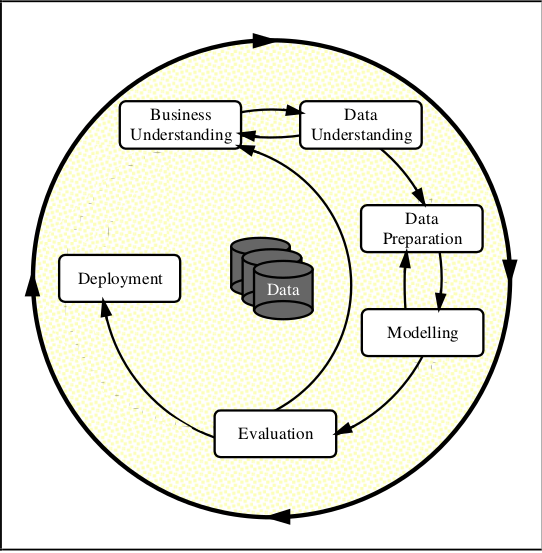
\includegraphics[scale=0.3]{imagenes/crisp}
    \caption[Diagrama CRISP-DM]{Diagrama CRISP-DM\\Fuente: \citep{Wirth00crisp-dm:towards}}
\end{figure}
	
	\negspacechap
\chapter{MARCO TEÓRICO}
	\negspacesec
	\section{SISTEMAS DE CONDUCCIÓN AUTÓNOMA}
    Un sistema de conducción autónoma es una combinación de varios componentes o subsistemas donde las tareas de percepción, toma de decisiones y operación de un vehículo son desarrolladas por un sistema electrónico en lugar de un conductor humano.
    
    \subsection{TAREAS DE LA CONDUCCIÓN AUTÓNOMA}
    Para lograr la conducción autónoma, se deben dividir tareas modulares, esto con el fin de poder realizar pruebas de cada componente y en caso de fallos, poder detectarlos aisladamente y que no afecten a los demás componentes.
    
    Las tareas son:
    \begin{itemize}[nosep]
        \item \textbf{Control lateral:} Control de la dirección o volante del vehículo.
        \item \textbf{Control longitudinal:} Control de la aceleración y freno.
        \item \textbf{Detección y respuesta de eventos y objetos:} (OEDR por sus siglas en inglés) detección de objetos importantes en la carretera como carriles y vehículos, también objetos fuera de la carretera como peatones o señales de tránsito. Como respuesta debe reaccionar a distintas situaciones peligrosas tanto deteniendo el coche o sacándolo de esa situación.
        \item \textbf{Planeamiento:} A corto plazo son las acciones inmediatas que debe tomar y modificar el camino ante adversidades, y a largo plazo es el mejor camino encontrado desde el origen al destino definido por el usuario.
    \end{itemize}
    estas están definidas en el documento de recomendaciones para vehículos autónomos de la Sociedad Internacional de Ingenieros de Automoción (SAE por sus siglas en inglés). \citep{J3016_201806}
    % \subsection{NIVELES DE AUTONOMÍA}
    % https://www.nhtsa.gov/technology-innovation/automated-vehicles-safety
    \subsection{ARQUITECTURA DE LA CONDUCCIÓN AUTÓNOMA}
    La arquitectura del software para la conducción autónoma se basa en una fase de adquisición de datos para entrenar los modelos predictivos y ajustar los algoritmos, y a partir de ahí una fase de inferencia, la cual tiene cuatro componentes principales:
    
    \begin{itemize}[nosep]
        \item \textbf{Percepción del ambiente:} Aquí se encuentran todos los modelos y algoritmos que nos permiten detectar objetos de interés a través de los sensores disponibles.
        \item \textbf{Mapeo del ambiente:} Una vez extraídos los objetos de interés, se procede a ubicarlos en posiciones relativas al vehículo.
        \item \textbf{Planificación de movimiento:} Se procede a armar un plan de acción para el estado del ambiente que se percibe en ese instante.
        \item \textbf{Control:} Una vez se realiza el plan de acción, se ejecuta enviando la información a los controladores de aceleración, freno y dirección.
    \end{itemize}
	
	\subsection{CARLA}
		CARLA es un simulador de código libre, desarrollado sobre Unreal Engine 4, para la investigación de la conducción autónoma, al ser pensado para esta tarea, provee una interfaz de comunicación a través de código en C++ y Python mediante su librería. Cuenta con distintos tipos de climas desde el día despejado hasta tardes lluviosas además de distintos modelos de vehículos y pedestres para lograr una simulación realista.
		
		La funcionalidad más importante de carla es poder extraer la imagen de cámaras y sensores virtuales para generar datos de entrenamiento, y poder controlar el vehículo mediante código para realizar pruebas de modelos aprendidos \citep{Dosovitskiy17}.
		
	\subsection{NIVELES DE CONDUCCIÓN AUTÓNOMA}
	\begingroup
%	\baselinestretch{1em}
	\setstretch{1.2}
	\begin{center}
		\footnotesize
%		\scriptsize
		\begin{tabularx}{\textwidth}{|l|X|}
			\hline
			\textbf{Nivel de automatización} & \textbf{Tareas} \\
			\hline
			Nivel 0 & No existe ningún tipo de automatización y el conductor humano se encarga de todo. \\
			\hline
			Nivel 1 & El sistema puede realizar el control longitudinal (aceleración) o lateral (giro), no ambos. \\
			\hline
			Nivel 2 & El sistema puede realizar el control longitudinal (aceleración) y lateral (giro). \\
			\hline
			Nivel 3 & Puede realizar el control del nivel 2 más cambios de carriles y reacción ante situaciones adversas en ciertos tipos de ambientes para los que se programó, cuando detecta que ya no está en un ambiente conocido se desactiva. \\
			\hline
			Nivel 4 & Puede realizar todo lo descrito en el nivel 3 y aparte cuando detecta algún tipo de falla o sale de un ambiente conocido, lleva al vehículo a un lugar seguro para desactivarse y que el usuario tome el control. \\
			\hline
			Nivel 5 & Puede realizar una conducción autónoma total, invariante a cualquier situación y lugar. \\
			\hline
		\end{tabularx}
		 
		\captionof{table}[Niveles de Conducción Autónoma]{niveles de conducción autónoma Fuente:\citep{J3016_201806}}\label{niveles}
	\end{center}
	\endgroup
	\vspace{-4mm}	
	La Sociedad de Ingenieros de Automoción internacional definió 5 niveles de conducción autónomas con sus características.
	
	Se considera como nivel básico de conducción autónoma a las tareas de control descrito en el nivel 2.
	
	\pospacesec
	\section{VISIÓN COMPUTACIONAL}
    
    \subsection{PROCESAMIENTO DE IMÁGENES}
        Es la aplicación de operaciones del procesamiento de señales unidimensionales sobre imágenes, interpretadas como una señal bidimensional.
        
        \subsubsection{REPRESENTACIÓN DE IMÁGENES EN UNA COMPUTADORA}
        Una imagen $I$ está compuesta por píxeles $(x, y, v)$ cuyos componentes son una coordenada $(x, y) \in \mathbb{Z}^2$ y un valor $v \in \mathbb{Z}^c$, con $c$ el número de canales de color, siendo $c=1$ una imagen a escala de grises y $c=3$ una imagen a colores Rojo, Verde y Azúl (RGB por sus siglas en inglés), definida sobre un conjunto $\Omega$. 
        
        \begin{equation}
            \Omega = \{(x, y)| 1 \leq x \leq N_{columnas} \land 1 \leq y \leq N_{filas}\} \subset \mathbb{Z}^2
        \end{equation}
        
        la representación que se observa en la computadora se le llama modelo grid cell, donde cada píxel es un cuadrado pequeño o celda con una intensidad de grises o canales RGB \citep{10.5555/2584519} con valores $0 \leq I_{x, y} \leq 255$.
        
        Existen distintos tipos de imágenes con las que se suelte trabajar en el área de visión artificial, las más comunes son las ya citadas escalas de grises y RGB, sin embargo es común trabajar con imágenes binarias, es decir con valores 0 o 255, para la representación de máscaras o regiones de interés, al igual que espacios de color alternativos como HSV.

        \begin{figure}[H]
            \centering
            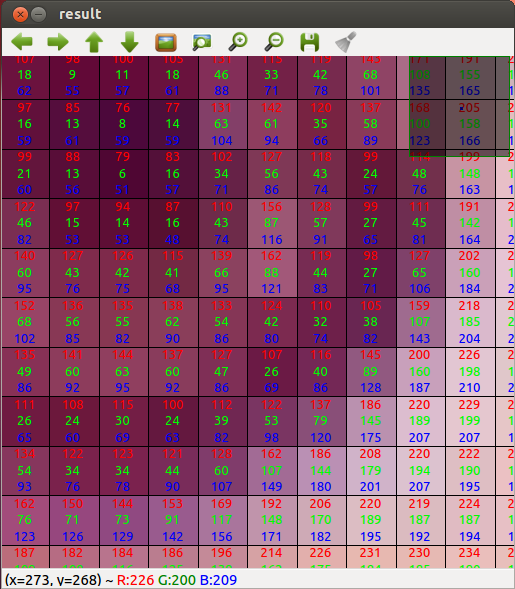
\includegraphics[scale=0.4]{imagenes/pixels}
            \caption[Intensidad de los canales de color RGB]{Intensidad de los canales de color RGB\\ Fuente: \citep{montabone_2012}}
        \end{figure}
		
        \subsubsection{CONVOLUCIÓN}
        Cuando se desea aplicar aplicar alguna transformación de alguna imagen $I$ a alguna imagen $I'$ como difuminados, realce de bordes o extracción de alguna característica, se debe aplicar un operador local lineal entre un filtro que acentúe la característica en la imagen $I$.
        
        El filtro denotado por $W$ es una matriz cuadrada de dimensión $(2k+1) \times (2k+1)$, aplicada en forma de ventana deslizante sobre cada pedazo de la misma dimensión de la imagen original, siendo $(x, y)$ el punto central de cada sección sobre la que se opera, se define la convolución como:
        
        \begin{equation}
            I'_{x,y} = \frac{1}{s} \sum_{i=-k}^{k} \sum_{j=-k}^{k} w_{i, j}\cdot I_{x+i, y+j}
        \end{equation}
        
        y se denota por el operador $*$ como $I' = I*W$ con $s$ un valor de escala \citep{10.5555/2584519}. Esta operación es equivalente a si se aplasta el filtro y la sección de la imagen en dos vectores, con el segundo vector al revés, y se realiza un producto punto o suma ponderada de sus valores.
        
        \begin{figure}[H]
        	\centering
        	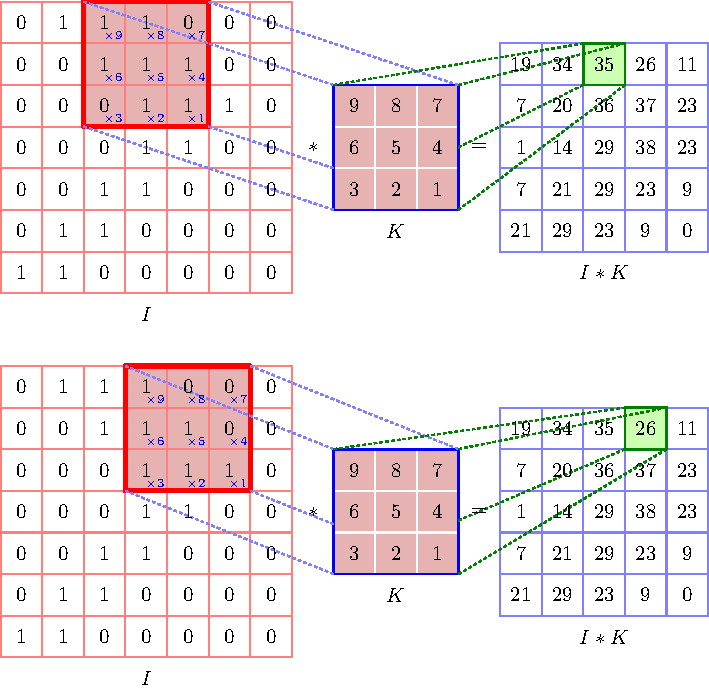
\includegraphics[scale=0.82]{imagenes/conv1}
        	\caption[Convolución del filtro $K$ con la imagen $I$]{convolución del filtro $K$ con la imagen $I$\\Fuente: elaboración propia}
        \end{figure}
    
    	\subsubsection{DETECCIÓN DE CONTORNOS}
    		
        
        \subsection{TRANSFORMACIONES MORFOLÓGICAS}
        	En tareas de imágenes binarias, el tipo más común de operaciones o filtros aplicados son las transformaciones morfológicas, llamadas así ya que modifican la estructura de los objetos binarios en la imagen, consisten en filtros llamados elementos estructurantes, los cuales son una matriz binaria que contiene un patrón bajo el cual se realiza una comparación o conteo píxel a píxel con recortes de la imagen, similar a una convolución 2D. \citep{szeliski}
			\subsubsection{DILATACIÓN}
				Es la operación que consiste en dilatar los píxeles, cuenta cuántos píxeles en el recorte de la imagen que estén en la misma coordenada que los unos del elemento estructurante son distintos de cero, si existe por lo menos un píxel que cumple esta condición entonces el píxel central de la ventana deslizante se le asignará el valor distinto de cero especificado.
				
				Gráficamente se puede interpretar como engrosar los trazos de algún objeto binario incrementando píxeles en los bordes.
				
				\begin{figure}[H]
					\centering
					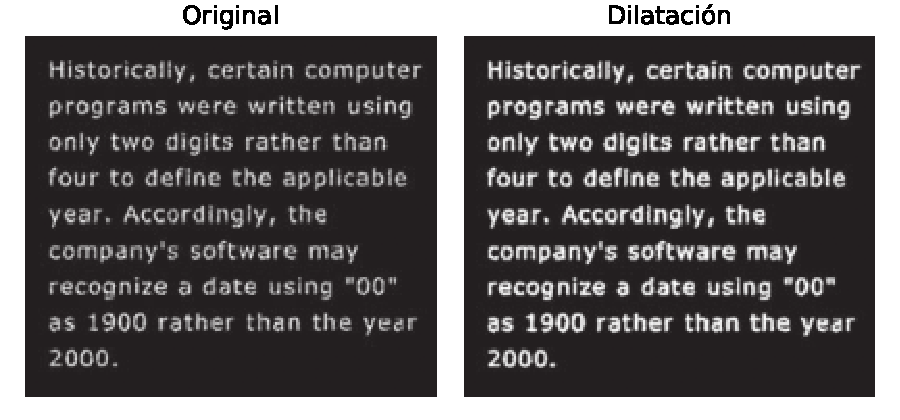
\includegraphics[scale=0.7]{imagenes/dilatacion}
					\caption[Dilatación sobre un conjunto de letras con discontinuidades]{dilatación sobre un conjunto de letras con discontinuidades\\Fuente: \citep{gonzalez}}
				\end{figure}	
						
			\subsubsection{EROSIÓN}
				Es la operación inversa a la dilatación, para esta operación, se realiza el mismo conteo de píxeles distintos de cero que encajen con la estructura del elemento estructurante, pero se asigna un valor positivo al centro solamente si el conteo es igual al número de elementos distintos de cero del filtro.
				
				\begin{figure}[H]
					\centering
					
\includegraphics[scale=0.7]{imagenes/erosion}
					\caption[Erosión de una letra]{erosión de una letra\\Fuente: \citep{szeliski}}
				\end{figure}
				
				El resultado gráfico de esta operación es equivalente a reducir los bordes de los objetos haciéndolos más delgados o pequeños.
			\subsubsection{APERTURA}
				Es una operación que combina erosión seguido de dilatación en un solo paso, se usa para eliminar pequeños artefactos que no pertenecen a los objetos de interés que se buscan extraer, como ruido o falsas detecciones discontinuas.
				
				\begin{figure}[H]
					\centering
%					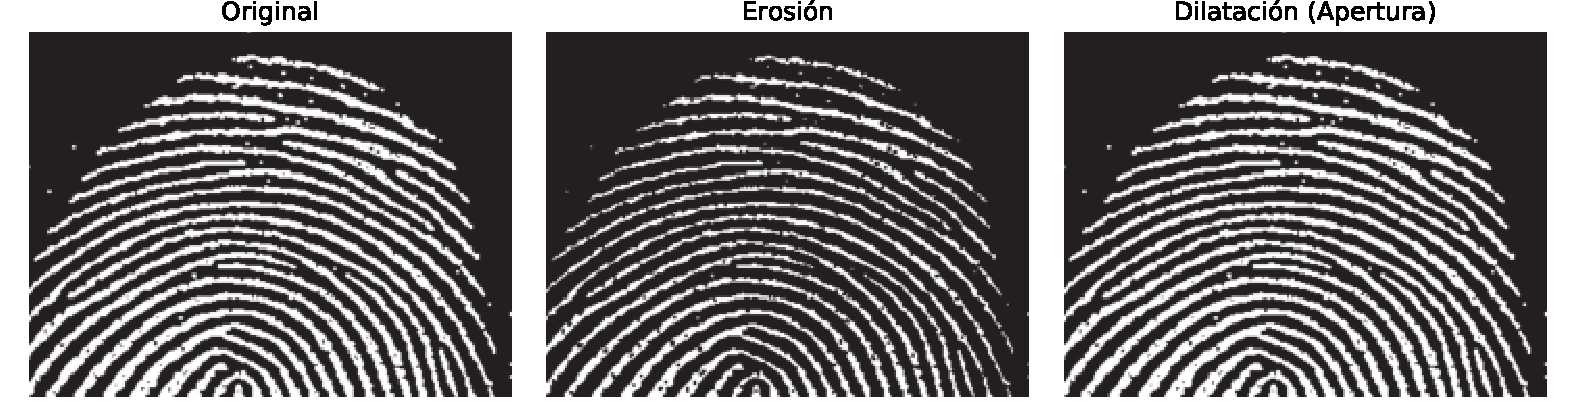
\includegraphics[scale=0.6]{imagenes/apertura}
					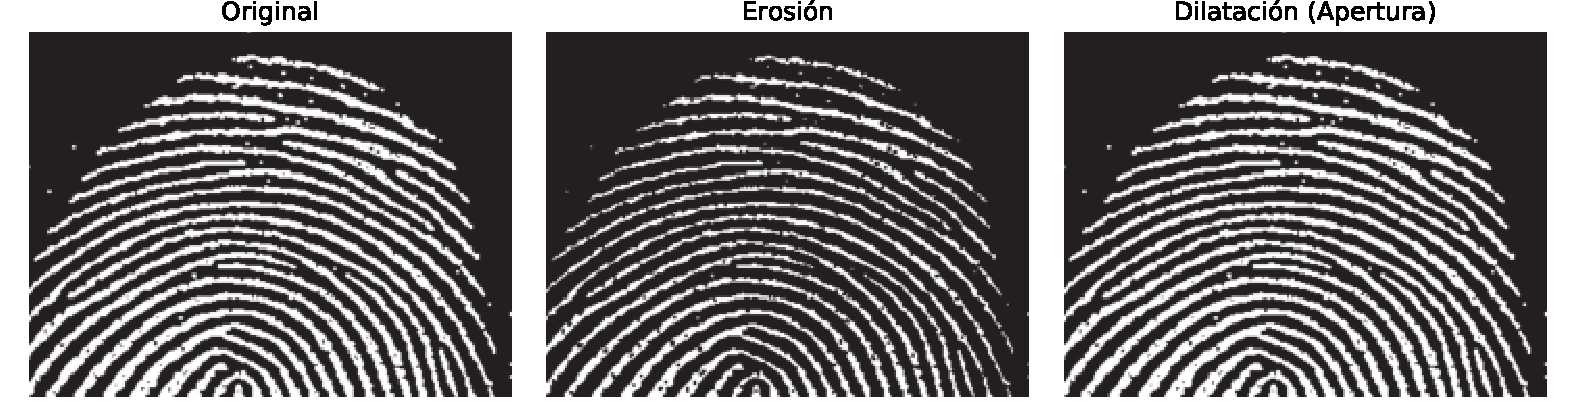
\includegraphics[scale=0.4]{imagenes/apertura}
					\caption[Apertura aplicada a una huella digital]{apertura aplicada a una huella digital para eliminar artefactos\\Fuente: \citep{gonzalez}}
				\end{figure}
				
				Al aplicar primero una erosión, se eliminan fragmentos discontinuos de menos píxeles que el tamaño de la ventana pero también se reduce el grosor de los objetos de interés, así que se aplica una dilatación, como los artefactos ya desaparecieron para ese momento, simplemente se restauran los objetos que pasaron la fase de erosión.
        \subsection{K-MEANS}
        	En español K-Medias, es un algoritmo nacido en el ámbito del procesamiento de señales y usado ampliamente en minería da datos para particionar un conjunto de $n$ observaciones en $k$ conglomerados o clusters, con el fin de clasificar a qué grupo pertenece cada observación o extraer información relevante de la relación entre los puntos de un mismo subconjunto.
        	
        	Debido a que se pretende que el algoritmo sea quien extraiga la información de los datos, la única entrada que se le provee es el número de clusters esperados, en base al cual se inicializan $k$ puntos aleatorios representando los centros de cada conglomerado. Al inicializarse aleatoriamente, se deben mejorar iterativamente las coordenadas de los centroides o medias denominados $\mu_i$.
        	
        	Se define una matriz binaria $R$ de dimensiones $m\times k$ dónde $m$ es el número de observaciones, esta matriz codifica en cada fila, representando a cada observación, el cluster al que pertenece, mediante un $1$ en la colúmna del cluster $i$ y $0$ en las demás. A cada elemento de $R$ se lo denominará como $r_{ij}$.
        	
        	Se busca minimizar la distancia entre elementos de cada cluster, es decir la distancia de una observación con su respectivo centroide, esto se hace optimizando la función de costo:
        	
        	\begin{equation}
        		J = \sum_{i=1}^m\sum_{j=1}^k r_{ij}||x_i - \mu_j||^2
        	\end{equation}
        	
        	La minimización de $J$ se hace mediante dos etapas hasta convergencia. Primero la asignación de centroides a cada punto mediante la regla:
        	
        	\begin{equation}
        		r_{ij} = 
        		\begin{cases}
        			1 & si\hspace{2mm}j = \underset{p}{argmin}||x_i - \mu_p||\\
        			0 & e.o.c
        		\end{cases}
        	\end{equation}
        
        	seguido del cómputo de nuevos centroides mediante el cálculo de la media de los puntos asignados al cluster $j$ en la anterior etapa \citep{bishop}.
        	
        	\begin{equation}
        		\mu_j = \frac{\sum_{i}r_{ij}x_i}{\sum_{i}r_{ij}}
        	\end{equation}
        
        	\begin{figure}[H]
        		\centering
%        		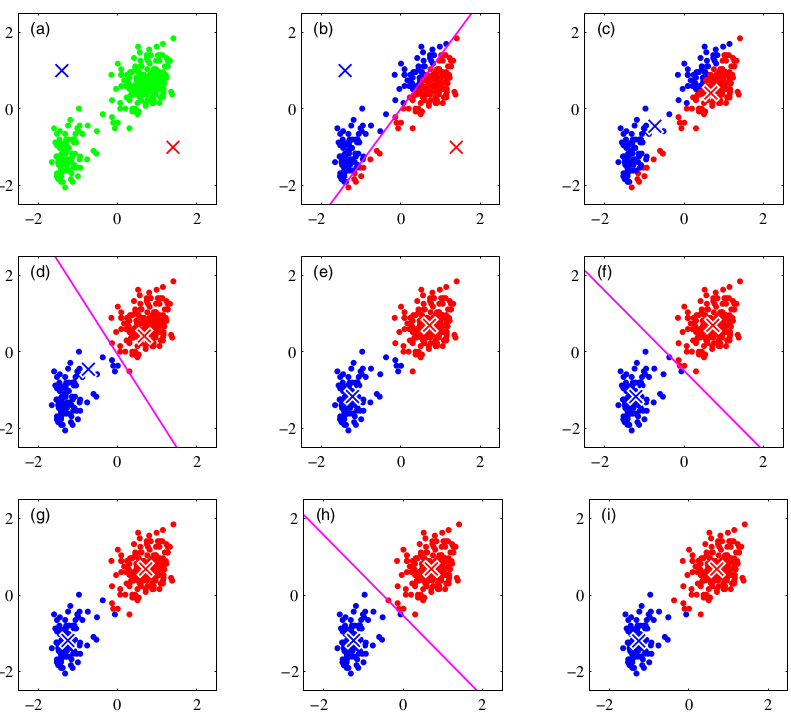
\includegraphics[scale=0.5]{imagenes/kmeans}
				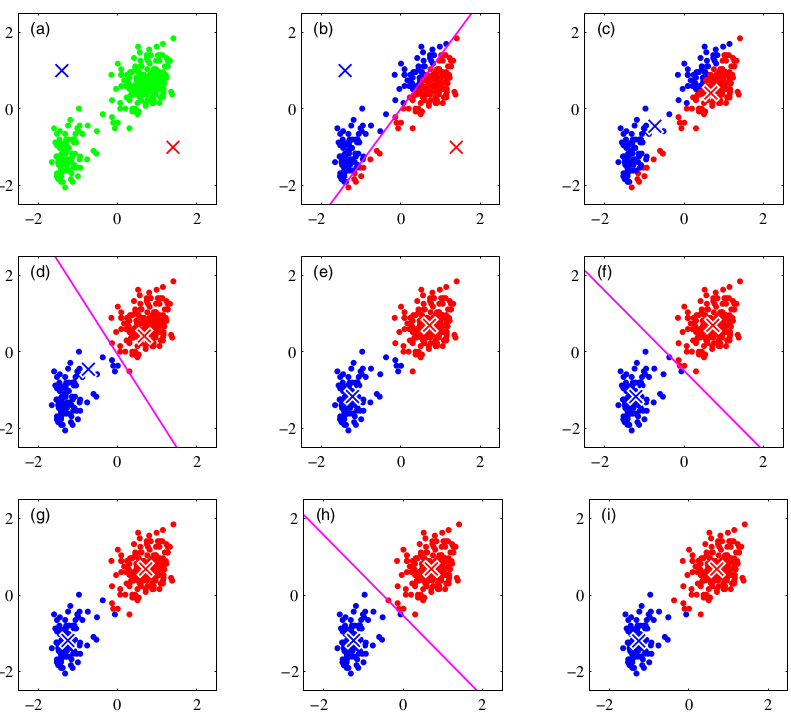
\includegraphics[scale=0.31]{imagenes/kmeans}
        		\caption[Ajuste iterativo de k-means]{ajuste iterativo de k-means\\Fuente: \citep{bishop}}
        	\end{figure}
        \subsection{FLOOD FILL}
        	Este algoritmo se usa cuando se desea rellenar un área delimitada por ciertos valores en una matriz, todas las herramientas de rellenado de color en programas de edición de imágenes usan una implementación.
        	
        	Consiste en recorrer recursivamente la matriz, marcando las posiciones ya visitadas hasta que ya no tenga a dónde ir, esta condición se cumple cuando todas las casillas de alrededor ya están marcadas como visitadas o de algún valor distinto al que se busca \citep{halim2013competitive}.\\
        	
        	{\setstretch{1.0}
        		\begin{algorithm}[H]
        			\caption{\textit{Flood Fill}}
        			\SetAlgoLined
        			\KwData{$mat:$ Matriz de valores}
%        			\KwData{$x, y:$ coordenada actual}
        			\KwData{$y:$ coordenada vertical actual}
        			\KwData{$x:$ coordenada horizontal actual}
        			\KwData{$d:$ vector de direcciones}
        			\vspace{2mm}
        			\If{mat[$ y $][$x$] $\neq$ val}{
        				mat[$ y $][$x$] = marca \tcp*{se marca como visitado}
        				\For{i $\rightarrow$ \textbf{length} d}{
        					flood\_fill($mat$, $y$+d[$ i $].y, x+d[$ i $].x)
        				}
        			}
        			\tcc{si ya está visitado finaliza la rama de recursión}
        		\end{algorithm}
        	}
        	
%        \subsubsection{DIFUMINADO}
%        Para aplicar un difuminado o blur a una imagen se aplica comúnmente un filtro normal o gaussiano, para esto se define que el filtro se distribuye normal bivariante:
%        
%        \begin{equation}
%            W \sim \mathcal{N}\left(\mu=\begin{bmatrix}
%                                    0\\
%                                    0
%                                    \end{bmatrix},
%                                    \Sigma=
%                                    \begin{bmatrix}
%                                    \sigma^2 & 0\\
%                                    0 & \sigma^2
%                                    \end{bmatrix}\right)
%        \end{equation}
%        
%        Si generamos un filtro o kernel como una muestra de la distribución normal, de tamaño $6\sigma-1$ redondeado al entero impar más cercano, por la regla empírica de las tres desviaciones estándar, y escalado por $\frac{1}{s}$, obtenemos el un filtro que ponderará más los píxeles cercanos al centro, de manera que el difuminado mantendrá las características de cada sección de la imagen.
%        
%        \begin{figure}[H]
%            \centering
%            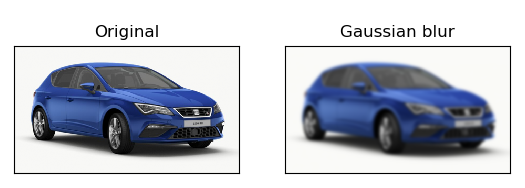
\includegraphics[scale=0.48]{imagenes/blur}
%            \caption{aplicación del filtro gaussiano\\ Fuente: Elaboración propia}
%        \end{figure}
%        % {\centering Fuente: Elaboración propia\par}
%        \subsubsection{DETECCIÓN DE BORDES}
%        Un borde es esencialmente un cambio brusco de intensidad de los valores de los píxeles en una sección de una imagen, de esta manera, para detectar bordes debemos aplicar algún tipo de suma ponderada que dé como resultado un valor alto si existe un cambio brusco de intensidad, y un valor bajo en caso contrario. 
%        Es bajo esta premisa que se propone el filtro Sobel \citep{sobel}, usado luego de aplicar un difuminado gaussiano, y consiste en una combinación entre una convolución gaussiana
%        $$\mathcal{G} = \begin{bmatrix}
%                                    1\\
%                                    2\\
%                                    1
%                        \end{bmatrix}$$
%        \noindent y una aproximación de la derivada parcial de la imagen en espacio discreto con $\Delta_x = \Delta_y = 1$ en cada dimensión
%        
%        $$\frac{\partial I_{x, y}}{\partial x} = \frac{I_{x+\Delta_x, y} - I_{x-\Delta_x, y}}{\Delta_x}$$
%        
%        $$\frac{\partial I_{x, y}}{\partial y} = \frac{I_{x, y+\Delta_y} - I_{x, y-\Delta_y}}{\Delta_y}$$
%        
%        \noindent dando como filtro unidimensional
%        
%        $$\mathcal{D} = \begin{bmatrix}
%                                    1 & 0 & -1
%                        \end{bmatrix}$$
%                        
%        \noindent combinando ambos filtros unidimensionales obtenemos el filtro Sobel para cada dimensión
%        \begin{equation}
%        \begin{aligned}
%        S_x &=  \begin{bmatrix}
%                 1\\
%                 2\\
%                 1
%                 \end{bmatrix}
%                 \begin{bmatrix}
%                 1 & 0 & -1
%                 \end{bmatrix}=
%                 \begin{bmatrix}
%                 1 &  0 &  -1\\
%                 2 &  0 &  -2\\
%                 1 &  0 &  -1\\
%                 \end{bmatrix}\\
%        S_y &=  \begin{bmatrix}
%                 1\\
%                 0\\
%                 -1
%                 \end{bmatrix}
%                 \begin{bmatrix}
%                 1 & 2 & 1
%                 \end{bmatrix}=
%                 \begin{bmatrix}
%                 1 &  2 &  1\\
%                 0 &  0 &  0\\
%                 -1 &  -2 &  -1\\
%                 \end{bmatrix}
%        \end{aligned}
%        \end{equation}
%        
%        \noindent al ser esta la derivada parcial con respecto de cada dirección, podemos calcular la magnitud mediante la norma $L_2$
%        
%        \begin{equation}
%            \nabla I_{x, y} = \sqrt{S_x^2 + S_y^2}
%        \end{equation}
%        
%        \noindent y la dirección del gradiente
%        
%        \begin{equation}
%            \theta = tan^{-1}\left(\frac{S_y}{S_x}\right)
%        \end{equation}
%        
%        \begin{figure}[H]
%            \centering
%            % 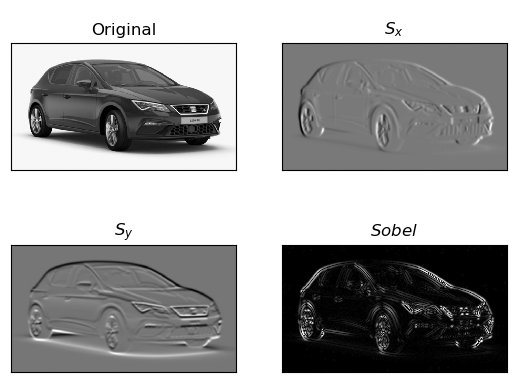
\includegraphics[scale=0.5]{imagenes/sobel_filters}
%            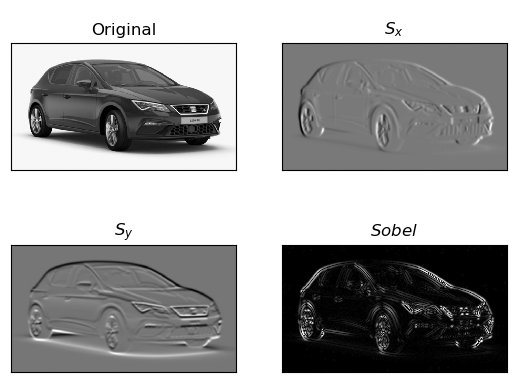
\includegraphics[scale=0.47]{imagenes/sobel_filters}
%            \caption{filtro Sobel por dimensiones y total\\ Fuente: Elaboración propia}
%        \end{figure}
%        % \vspace{-8mm}
%        % \begin{center}
%        %     Fuente: Elaboración propia
%        % \end{center}
%        \subsubsection{FILTRO CANNY}
%        Los bordes detectados por el filtro Sobel no son independientes de la resolución, por lo que pueden ser más gruesos o delgados dependiendo de la imagen, y detectar como bordes transiciones de iluminación que no lo son necesariamente, es con el fin de refinar este resultado que propone el filtro Canny, que se aplica a la salida de un filtro Sobel \citep{canny}.
%        Para aplicar este filtro primero se redondean las direcciones a múltiplos de $45^\circ$ y se procede a verificar si comparado con los píxeles vecinos en esa sección y esa orientación, es el valor máximo o no, en caso que no lo fuese se anula el valor del píxel volviéndolo $0$, caso contrario se continúa con el paso de probar límites de valores, dónde se eligen dos valores $t_{alto}$ y $t_{bajo}$, si un píxel cumple $I_{x,y} \ge t_{alto}$ entonces se considera borde, entonces se verifica cuáles de los 8 píxeles vecinos cumplen $I_{x\pm 1, y \pm 1} \ge t_{bajo}$, finalmente los píxeles que cumplan esta condición se marcan con el máximo valor de un píxel, $255$ y se repite el procedimiento. Si no se cumple la primera condición con el límite alto se asigna el valor $0$ al píxel, obteniendo así una imagen binaria donde los píxeles que representan un borde son de color blanco y los que no, son negros.
%        
%        \begin{figure}[H]
%            \centering
%            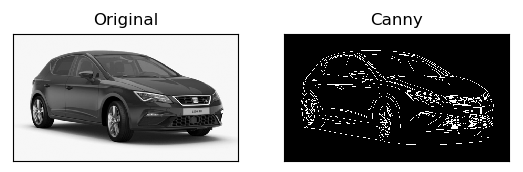
\includegraphics[scale=0.55]{imagenes/canny}
%            \caption{aplicación del filtro Canny\\ Fuente: Elaboración propia}
%        \end{figure}

	
	\section{APRENDIZAJE AUTOMÁTICO}
    Del inglés Machine Learning, son métodos basados en la experiencia (datos) que aprenden características de la información disponible para realizar predicciones acertadas \citep{10.5555/3360093}.
    \subsection{APRENDIZAJE SUPERVISADO}
        Es un tipo de tarea de aprendizaje que consiste en extraer características representativas de un conjunto de datos $\mathcal{D}$ y obtener algún mapeo de cada observación $x_i$ a su correspondiente $y_i$, dónde se conocen los $y_i$.
    
        \subsubsection{APRENDIZAJE CORRECTO PROBABLEMENTE APROXIMADO}
        En una tarea de aprendizaje supervisado se tiene un conjunto de datos $\mathcal{D}$ el cual sigue una distribución conjunta
        
        $$\mathcal{D} \sim P(x, y)$$
        
        \noindent con $\mathbf{X}$ el conjunto de observaciones y $\mathbf{Y}$ las etiquetas o valores a predecir. La distribución de los datos es desconocida, por lo que se considera a $\mathcal{D}$ como una muestra aleatoria de tamaño $m$ proveniente de esta distribución.
        
        Con el fin de poder modelar estos datos y aproximarse a la distribución original para poder realizar inferencias, se define una función predictiva
        
        $$f: \mathbf{X} \mapsto \mathbf{\hat{Y}}$$
        
        \noindent la cual es parte de una familia de funciones o espacio de hipótesis $\mathcal{H}$ definido por un modelo paramétrico, que se ajustan al conjunto de datos con distintos porcentajes de exactitud, dando como salida el valor esperado dado de $y_i \in \mathbf{Y}$ dado $x_i \in \mathbf{X}$.
        
        $$\hat{y}_i = E(y_i|x_i) = f(x_i)$$
        
        La tarea de aprender consiste en elegir la mejor función $f^* \in \mathcal{H}$, que minimice la esperanza de una función de pérdida $\mathcal{L}(\hat{y}_i, y_i)$. Esta función es una métrica definida en $\mathbb{R}$ que permite medir cuán lejos está nuestra predicción $\hat{y}_i$ de un valor esperado conocido $y_i$.
        
        Para obtener la función objetivo se minimiza el riesgo:
        
        \begin{equation}
        \begin{aligned}
            f^* &= \underset{f \in \mathcal{H}}{\text{argmin}} \text{ } E\left[\mathcal{L}(f(\mathbf{X}), \mathbf{Y})\right]\\[1.4em]
            &= \int_\mathbf{X} \mathcal{L}(f(x_i), y_i)dP(\mathbf{X}, \mathbf{Y})
        \end{aligned}
        \end{equation}
        
        \noindent sin embargo no es posible calcular esta integral ya que no se conoce la distribución, por lo que se minimiza el riesgo empírico
        
        \begin{equation}
            \hat{f} = \underset{f \in \mathcal{H}}{\text{argmin}} \frac{1}{m} \sum_{i=1}^m \mathcal{L}(f(x_i), y_i)
        \end{equation}
        
        \noindent el cual también se conoce como función de costo. \citep{10.5555/3360093}
        
    \subsection{REGRESIÓN}
        Uno de los tipos más importantes de tareas de aprendizaje automático es la regresión, en que la variable respuesta es continua, es decir $y_i \in \mathbb{R}$.
        \subsubsection{REGRESIÓN LINEAL}
        Es un modelo que estudia la correlación lineal entre las variables predictoras y las variables predichas, de manera que ajusta el mejor hiperplano (en el caso bidimensional la mejor línea), que modele la correlación lineal de los datos. \citep{gujarati2003basic}
        
        El modelo de regresión lineal se define como:
        
        \begin{equation}
            \mathrm{y}_i = \mathbf{\theta}\cdot\mathbf{x}_i + \varepsilon_i = \theta_0 + \theta_1\mathrm{x}_{i1} + \dots + \theta_n\mathrm{x}_{i n} + \varepsilon_i
        \end{equation}
        
        dónde $\mathrm{x}_{i j}$ es una entrada de la matriz de regresores $\mathbf{X}$ con $m$ observaciones y $n$ características, en la cual el índice $i$ representa el número de observación y $j$ el número de característica para esa observación, $\theta_j$ es un parámetro correspondiente a la $j$-ésima característica el cual representa el grado de incidencia que tiene este atributo sobre la predicción y $\varepsilon_i$: es un término de error que no se puede explicar con las características de nuestros datos o variables regresoras.
        
        \noindent De esta manera se puede reescribir el modelo de manera matricial como:
        
        \begin{equation}
            \mathbf{y} = \mathbf{X}\cdot\mathbf{\theta} + \mathbf{\varepsilon}\label{eq:3}
        \end{equation}
        
        \noindent con los parámetros
        
        $$\theta = \begin{bmatrix}
        	\theta_0 & \theta_1 & \dots & \theta_n
        \end{bmatrix}$$
    
    	\noindent y con
        
        $$\mathbf{X} = \begin{bmatrix}
                        1 & x_{11} & x_{12} & \dots & x_{1n}\\
                        1 & x_{21} & x_{22} & \dots & x_{2n}\\
                        \vdots & & & \ddots & \\
                        1 & x_{m1} & x_{m2} & \dots & x_{mn}\\
                        \end{bmatrix}$$
        
%        \noindent y los parámetros
        
%        $$\theta = \begin{bmatrix}
%                    \theta_0\\
%                    \theta_1\\
%                    \vdots\\
%                    \theta_n
%                    \end{bmatrix}$$
                    
        \noindent con función predictora
        
        \begin{equation}
            \mathbf{\hat{Y}} = f(\mathbf{X}) = \mathbf{X}\cdot\mathbf{\theta}
        \end{equation}
        
        Los parámetros $\theta$ que permiten encontrar la función $\hat{f}$ se estiman mediante el método de mínimos cuadrados con función de pérdida $\mathcal{L} =  (\mathrm{y}_i - \mathrm{\hat{y}}_i)^2$, y función de costo
        
        \begin{equation}
            E(\theta) = \frac{1}{m} (\mathrm{y}_i - \mathrm{\hat{y}}_i)^2 = \frac{1}{m} (\mathbf{y} - \mathbf{\hat{y}})^\prime\cdot (\mathbf{y} - \mathbf{\hat{y}})
        \end{equation}
        
        \noindent dónde el apostrofe representa la operación de trasposición para el caso matricial.
        
        Desarrollando esta fórmula, derivando e igualando a 0 para encontrar el mínimo, se obtiene una fórmula para calcular los parámetros
        
        \begin{equation}
            \hat{\theta} = (\mathbf{X}^\prime\cdot\mathbf{X})^{-1}\cdot\mathbf{X}^\prime\cdot\mathbf{y}
        \end{equation}
        
        \noindent es así como se obtiene la mejor función predictora estimada $\hat{f} = \mathbf{X}\cdot\hat{\theta}$.
        
        \begin{figure}[H]
            \centering
%             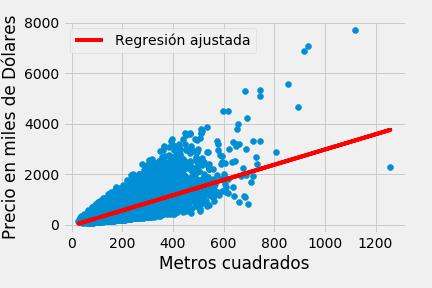
\includegraphics[scale=0.6]{imagenes/linear_fit}
            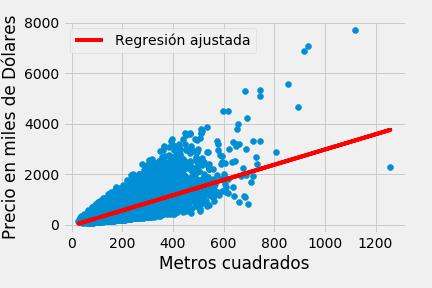
\includegraphics[scale=0.45]{imagenes/linear_fit}
            \caption[Ajuste de regresión lineal]{Ajuste de una regresión lineal a un conjunto de datos de precios de casas\\ Fuente: Elaboración propia}
        \end{figure}
    	
    	\vspace{-10mm}
    	\subsubsection{REGRESIÓN GENERALIZADA}
    		Si se aplica una función $\mathbb{R}^n\mapsto\mathbb{R}$ antes de obtener la predicción, y se optimiza en base a esta definción, se obtienen variantes de la regresión denominados modelos lineales generalizados.
    		
    		Un ejemplo de caso categórico es la regresión logística, pero existen distintos otros modelos como la regresión Poisson o incluso la predicción de una regresión con variable de salida en un rango $(-1, 1)$ definida por una tangente hiperbólica.
    		
    	\subsubsection{MEDIAS MÓVILES EXPONENCIALES}
    		Es un filtro aplicado a una señal o serie de tiempo, con el fin de promediar los valores en un tiempo $t$ de manera ponderada exponencialmente por los términos anteriores de la serie.
    		
    		Se aplica comúnmente para encontrar tendencias de los datos y para suavizar oscilaciones dadas por valores atípicos de poca duración en la señal.
    		
    		Al depender de valores previos de la serie, se calcula de manera recursiva con la fórmula
    		
    		\begin{equation}
    			S_t = \begin{cases}
    				y_0, & t=0\\
    				\alpha y_t + (1 - \alpha)S_{t-1}, & t \ge 1
    			\end{cases}
    		\end{equation}
    	
    		definida por un parámetro $\alpha$ que a mayor valor descarta observaciones antiguas más rápido \citep{10.5555/3002669}.
    	
        % \vspace{-8mm}
        % \begin{center}
        %     Fuente: Elaboración propia
        % \end{center}
    \subsection{CLASIFICACIÓN}
        Cuando la variable respuesta es de tipo categórica, se considera una tarea de clasificación, en que dado un vector de entrada $\mathrm{x_i}$ se debe predecir cuál es la categoría a la que pertenece. \citep{hastie01statisticallearning}
        \subsubsection{REGRESIÓN SOFTMAX}
        Es un modelo lineal generalizado, el cual extiende la idea de la regresión lineal mediante la función de enlace logit multinomial, también llamada softmax, la cual es una generalización de la función sigmoide a múltiples clases, cuyo valor de salida es un vector de probabilidades excluyentes para cada fila de la matriz $\hat{Y}$
        
        \begin{equation}
            Softmax(Z) = \frac{e^{Z}}{\sum_{j=1}^{C} e^{Z_j}}
        \end{equation}
        
        \noindent dónde $Z = \mathbf{X}\cdot\theta$, con $\theta$ ahora de dimensiones $(n \times c)$ siendo $c$ el número de clases, de este modo, mientras mayor el valor de $Z_{i,j}$, mayor es la probabilidad al predecir la clase $j$. \citep{Goodfellow-et-al-2016}
        
        Gráficamente, se interpreta este modelo como el mejor hiperplano que separa el espacio en $c$ partes, donde cada parte contiene las observaciones de su correspondiente clase.
        
        \begin{figure}[H]
            \centering
            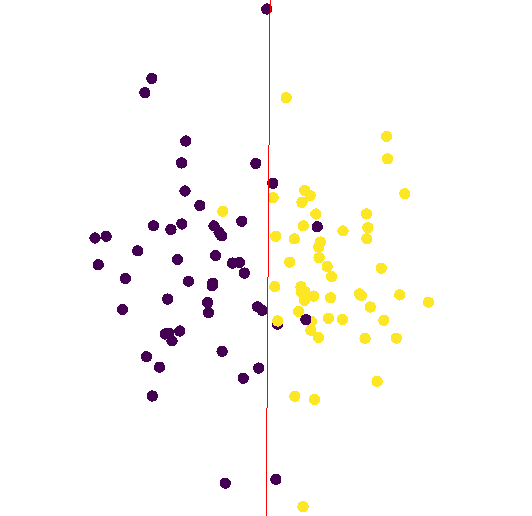
\includegraphics[scale=0.35]{imagenes/logistic_reg}
%			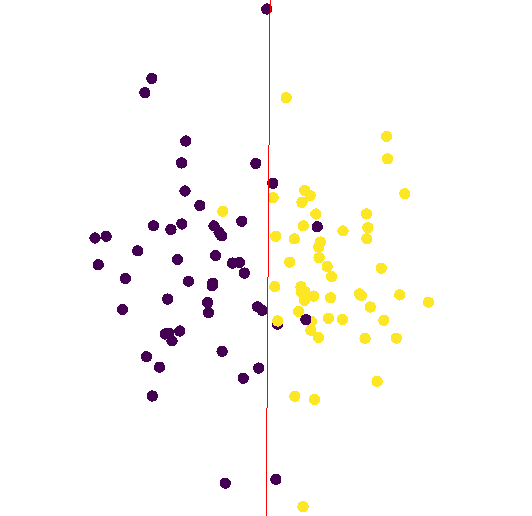
\includegraphics[scale=0.47]{imagenes/logistic_reg}
            \caption[Ajuste de regresión logística]{Ajuste de una regresión logística a un conjunto de datos con 2 clases\\ Fuente: Elaboración propia}
        \end{figure}
        % \vspace{-8mm}
        % \begin{center}
        %     Fuente: Elaboración propia
        % \end{center}
        Debido a la nolinealidad de la función de enlace, los parámetros ya no se pueden estimar de manera analítica, por lo que se debe usar un método iterativo para resolver el sistema, sin embargo, lo más importante y requisito de todos los métodos, es encontrar la derivada de la función de costo con respecto a los parámetros.
        
        Con el fin de tener una mejor medida del error para las probabilidades de las categorías, se usa la función log softmax
        
        \begin{equation}
            \mathcal{L} = -log(\hat{y})
        \end{equation}
        
        \noindent derivando por regla de la cadena $\frac{\partial\mathcal{L}}{\partial \theta} = \frac{\partial\mathcal{L}}{\partial Z} \cdot \frac{\partial Z}{\partial \theta}$, se obtiene
        
        \begin{equation}
            \frac{\partial\mathcal{L}}{\partial \theta} = X' \cdot (\mathbf{\hat{y}} - \mathbf{y})
        \end{equation}
        
        \noindent la derivada requisito para cualquier algoritmo de optimización.
        
    \subsection{DESCENSO DEL GRADIENTE ESTOCÁSTICO}
        Uno de los métodos más utilizados para resolver el sistema y encontrar los parámetros de modelos no lineales. Consiste en particionar el conjunto de datos en pequeños lotes, de modo que en cada iteración, se evalúa la derivada en cada lote y se mueven los valores de los parámetros en dirección al mínimo de la función \citep{hastie01statisticallearning}.
        
        \begin{figure}[H]
            \centering
%            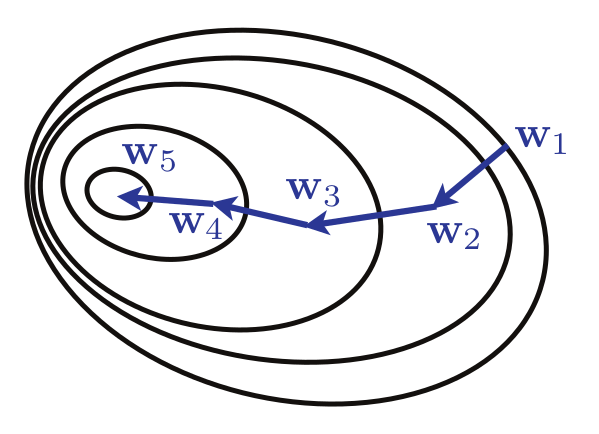
\includegraphics[scale=0.38]{imagenes/sgd}
			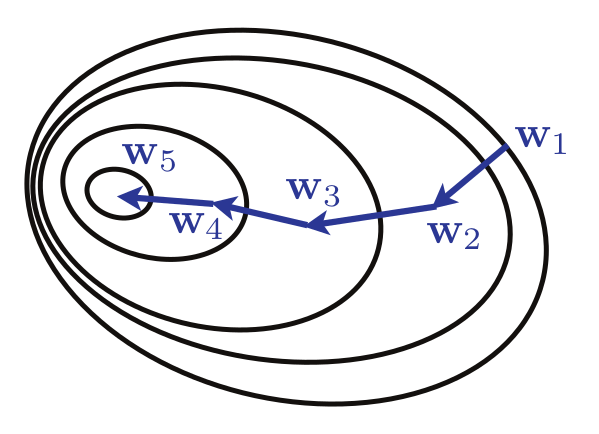
\includegraphics[scale=0.32]{imagenes/sgd}
            \caption[Pasos de los parámetros $W$ en cada iteración camino al mínimo error]{Pasos de los parámetros $W$ en cada iteración camino al mínimo error\\ Fuente: \citep{10.5555/3360093}}
        \end{figure}
      
        {\setstretch{1.0}
        \begin{algorithm}[H]
        	\caption{\textit{Descenso del Gradiente estocástico}}
        	\SetAlgoLined
        	\KwData{$\mathbf{X}:$ Matriz de observaciones}
        	\KwData{$\mathbf{Y}:$ Vector de valores a predecir}
        	\KwData{$\alpha:$ Tamaño del paso de aprendizaje}
        	\KwData{$b:$ Tamaño del lote}
        	\KwData{$f(\mathbf{X}, \theta):$ Función objetivo a optimizar}
        	Inicializar aleatoriamente $\mathbf{\theta}$\\
        	\While{$\mathbf{\theta}$ no converge}{
        		\For{$i$ $\to$ $\frac{m}{b}$}{
        		    $\mathbf{\theta} \leftarrow \mathbf{\theta} - \alpha\cdot \nabla f(\mathbf{X}_i, \theta)$
        		}
        	}
        	\Return $\theta$
        \end{algorithm}
        }
        
        \noindent dónde $\mathbf{\theta} \leftarrow \mathbf{\theta} - \alpha\cdot \nabla f(\mathbf{X}_i, \theta)$ es el gradiente en cada lote.
	\subsection{ADAM}
		Es una mejora del descenso del gradiente, la más utilizada debido a la mayor velocidad de convergencia.
		
		{\setstretch{1.0}
			\begin{algorithm}[H]
				\caption{\textit{Adam}}
				\SetAlgoLined
				\KwData{$\mathbf{X}:$ Matriz de observaciones}
				\KwData{$\mathbf{Y}:$ Vector de valores a predecir}
				\KwData{$\alpha:$ Tamaño del paso de aprendizaje}
				\KwData{$\beta_1$, $\beta_2$ $\in [0, 1)$ parámetros de las medias móviles}
				\KwData{$b:$ Tamaño del lote}
				\KwData{$f(\mathbf{X}, \theta):$ Función objetivo a optimizar}
				Inicializar aleatoriamente $\mathbf{\theta}$\\
				Inicializar en 0 $m$ \tcp*{vector de la media}
				Inicializar en 0 $v$ \tcp*{vector de la varianza}
				$n \leftarrow 0$\\
				\While{$\mathbf{\theta}$ no converge}{
					$n \leftarrow n + 1$\\
					\For{$i$ $\to$ $\frac{n\_observaciones}{b}$}{
						\vspace{1.5mm}
						$g \leftarrow \nabla f(\mathbf{X}_i, \theta)$ \tcp*{gradiente del i-ésimo lote}
						$m \leftarrow \beta_1\cdot m + (1-\beta_1)\cdot g$ \tcp*{MAE de la media}
						$v \leftarrow \beta_2\cdot v + (1-\beta_2)\cdot g\odot g$ \tcp*{MAE de la varianza}
						$\hat{m} \leftarrow \frac{m}{1-\beta_1^n}$ \tcp*{corrección del sesgo}
						$\hat{v} \leftarrow \frac{v}{1-\beta_2^n}$\\
						$\theta \leftarrow \theta - \alpha\cdot\frac{\hat{m}}{\sqrt{\hat{v}}+\varepsilon}$\\
					}
				}
				\Return $\theta$
			\end{algorithm}
		}
	
		El algoritmo aplica dos medias móviles exponenciales, una con parámetro $\beta_1$ para estabilizar las oscilaciones calculando la media del gradiente, y otra con $\beta_2$ estimar la varianza no central, usando la media de los gradientes al cuadrado debido a la relación.
		
		\begin{equation}
			E[X]^2 = E[X^2]	- Var[x]
		\end{equation}
		
		Dado que los momentos estimados son sensibles a la inicialización, se realiza una corrección de sesgo del estadístico estimado
		
		\begin{equation}
			\hat{\bar{X}} = \frac{\bar{X}}{1-\beta_i^n}
		\end{equation}
		
		con $n$ la n-ésima iteración, de esta forma el denominador tiende a $1$ conforme pasan las etapas de optimización.
	
	\section{APRENDIZAJE PROFUNDO}
    Buscando resolver el problema de la generalización e invarianza a los datos de los que sufren muchos modelos de machine learning o aprendizaje automático, es que nace el Deep Learning o aprendizaje profundo el cual propone apilar múltiples capas con varias neuronas cada una en una red neuronal para lograr representar funciones más complejas y altamente no lineales, a cambio de requerir muchos más datos para su entrenamiento. \citep{Goodfellow-et-al-2016}
    \subsection{PERCEPTRÓN MULTICAPA}
        El perceptrón multicapa, más conocido como red neuronale, extiende la idea de la regresión logística y lineal a un modelo de $n$-etapas, una especie de concatenación de regresiones con la diferencia que a la salida de las capas se les aplica una función $g(\mathbf{X})$ denominada función de activación, que consiste en alguna transformación no lineal de las variables de salida intermedias con el fin de poder realizar ajustes más complejos a los datos. \citep{hastie01statisticallearning}
        
        \begin{figure}[h]
            \centering
%           	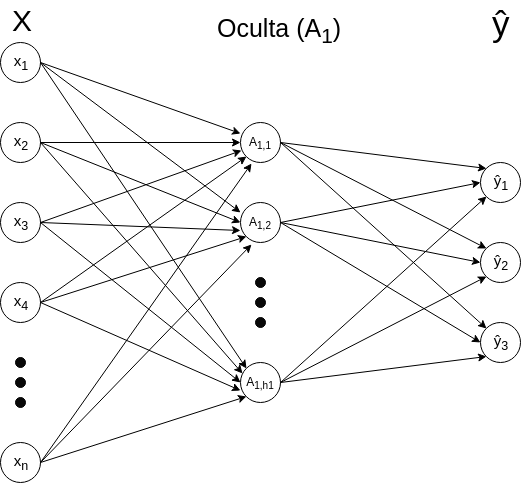
\includegraphics[scale=0.55]{imagenes/NeuralNetwork_bak}
            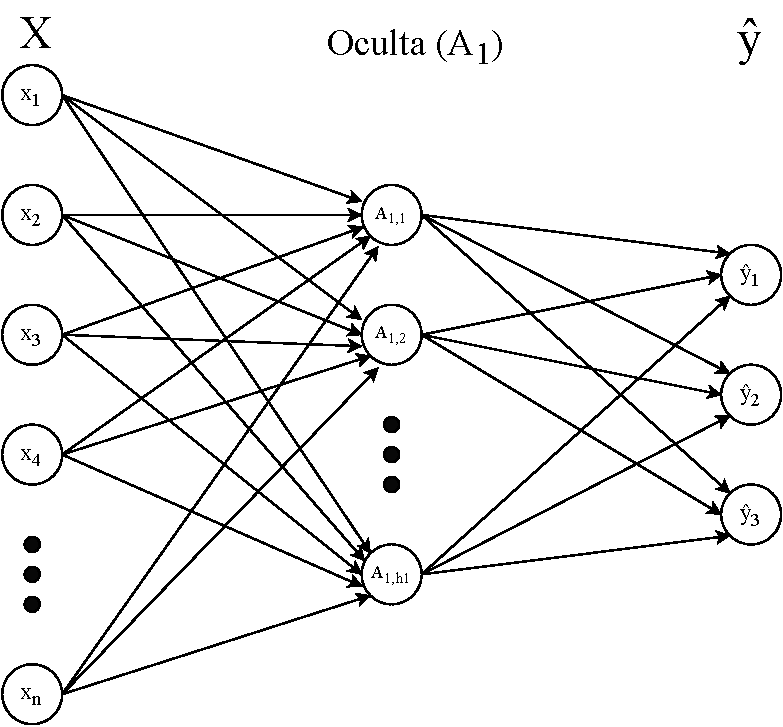
\includegraphics[scale=0.74]{imagenes/NeuralNetwork}
            \caption[Red neuronal con una capa oculta]{Red neuronal con una capa oculta\\Fuente: elaboración propia}
        \end{figure}
        % \vspace{-8mm}
        % \begin{center}
            % Fuente: elaboración propia
        % \end{center}  
        
        Conforme incrementa la cantidad de capas y parámetros de una red neuronal, esta puede aproximar funciones cada vez más complejas, por lo que se le denomina un aproximador universal de funciones, ya que el espacio $\mathcal{H}$ de todas las posibles funciones que puede aproximar, es infinito, es debido a esto que se requieren más observaciones en la muestra de la distribución de datos a modelar. \citep{Goodfellow-et-al-2016}
        
        La red neuronal matemáticamente es una composición de $n$ funciones o capas, aplicando una no linealidad $g(\mathbf{X})$ en cada etapa, con una función de enlace $g(\mathbf{X})$ en la capa de salida, la cual comúnmente es una softmax para clasificación o la identidad para regresión, siendo esta última etapa una regresión logística o lineal respectivamente, con variables de entrada procesadas por las anteriores capas de manera que sea linealmente aproximable en un número arbitrario de dimensiones elegidas por el modelo al entrenarse sobre los datos. La función de costo se denota por $J(\theta)$ con $\theta$ todos los parámetros del modelo. \citep{bishop}
        
        Basándonos en la definición de la matriz $\mathbf{X}$ descrita en el modelo de regresión lineal, la columna de unos agregada antes de ajustar el modelo para el parámetro constante, ahora se considerará como un vector de parámetros $b_k$ para las $l_k$ neuronas de la capa $k$, y los demás parámetros son representados por la matriz $W_k$.
%        Quedando definida la composición de funciones de la red neuronal como:
        
        \begin{equation}
	        \begin{aligned}
	            Z_1 &= X \cdot W_1 + b_1\\
	    		A_1 &= g_1(Z_1) \\
	    		Z_2 &= A_1 \cdot W_2 + b_2 \\
	    		A_2 &= g_2(Z_2) \\
	    		&\dots\\
	    		Z_n &= A_{n-1} \cdot W_n + b_n\\
	    		\hat{Y} &= h(Z_n) \\
	    		J(\theta) &= \sum_{i}^{m} \mathcal{L}(\hat{y_i}, y_i)
	        \end{aligned}
        \end{equation}
        
        
        
        \subsubsection{FUNCIONES DE ACTIVACIÓN}
        Con el fin de obtener aproximaciones no lineales a los datos, se debe evaluar la salida $Z_k$ de cada capa en una función de activación no lineal $g_k(Z_k)$.
        
        Las funciones de activación más comúnmente usada por ser fácil de computar y diferenciar es la \textit{Rectified Linear Unit} o \textbf{RELU} \citep{Goodfellow-et-al-2016}, la cual está definida por:
        \begin{equation}
            g(Z_k) = max(0, Z_k) \text{ $\forall$ $z_{k,j}$ / $j$ : $0, 1, ..., l_k$}
        \end{equation}
        
        \noindent cuya derivada con fines de estabilidad numérica es
        
        \begin{equation}
			\frac{\partial g(Z_k)}{\partial Z_k} = 
			\begin{cases}
			\text{1 si } z_{k,j} > 0\\
			\text{0 en otro caso}
			\end{cases}
		\end{equation}
        
        \subsubsection{RETROPROPAGACIÓN DE LOS ERRORES}
        Para ajustar los parámetros o entrenar la red neuronal, al tener más capas por las que pasar para obtener todos los gradientes de los errores, se debe derivar a través de cada una de ellas, a este algoritmo se le llama Backpropagation o Retropropagación, que es simplemente como su nombre dice, propagar los gradientes de reverso a través de la red neuronal.
		
		Primero se obtiene la derivada con respecto da cada uno de los parámetros de la composición de funciones por regla de la cadena
		
		\begin{equation}
		    \frac{\partial J}{\partial \theta_k} = \frac{\partial J}{\partial Z_n} \cdot  \frac{\partial Z_{n}}{\partial A_{n-1}} \cdot \frac{\partial A_{n-1}}{\partial Z_{n-1}} \cdot  \dots \cdot \frac{\partial A_{k}}{\partial Z_{k}} \cdot \frac{\partial Z_{k}}{\partial \theta_{k}}
		\end{equation}
		
		\noindent dónde $\theta_k$ representa cualquiera de los parámetros de $W_k$ o $b_k$ en la capa $k$, notese que para obtener la derivada con respecto de los parámetros en la capa $k$ se requiere la derivada en con respecto de las activaciones las capas siguientes, así, cuando se obtiene la derivada con respecto de los parámetros de la capa $k$ ya se calcula para todas las capas siguientes y sólo se debe multiplicar por la derivada de la salida lineal de la capa $k$ con respecto del parámetro $\theta_k$. \citep{bishop}
		
		Para el caso de regresión y clasificación con softmax $\frac{\partial J}{\partial Z_n} = (\mathbf{\hat{Y}} - \mathbf{Y})$ de forma vectorial, de manera general la derivada con respecto de algún parámetro está dada por
		
		\begin{equation}
		    \frac{\partial J}{\partial \theta_k} = \frac{\partial J}{\partial Z_n} \cdot \prod_{i=0}^{n-(k+1)} W_{n-i} \frac{\partial g_{n-(i+1)}(Z_{n-(i+1)})}{\partial Z_{n-(i+1)}} \cdot \frac{\partial Z_k}{\partial \theta_k}
		\end{equation}
		
		Similar a la regresión logística, se estiman los parámetros mediante un método de optimización, cuyo requisito sea la derivada con respecto a cada uno de los parámetros.
		
    \subsection{REDES NEURONALES CONVOLUCIONALES}
        Es un tipo de arquitectura de redes neuronales diseñada específicamente para tareas sobre imágenes, de manera que las operaciones sobre las observaciones de entrada ya no son composiciones realizando multiplicaciones matriciales, sino que cada neurona se convierte en un filtro o kernel de dimensiones $(k \times k)$, de los cuales se tienen varios filtros que se aplican sobre la imagen mediante la convolución.
        
        La idea detrás de este tipo de red es que se apliquen varios filtros en cada capa de la red para extraer características importantes de los objetos que se buscan, estos filtros se aprenden mediante retropropagación y ya no se diseñan a mano \citep{Goodfellow-et-al-2016}.
        
        \begin{figure}[H]
            \centering
            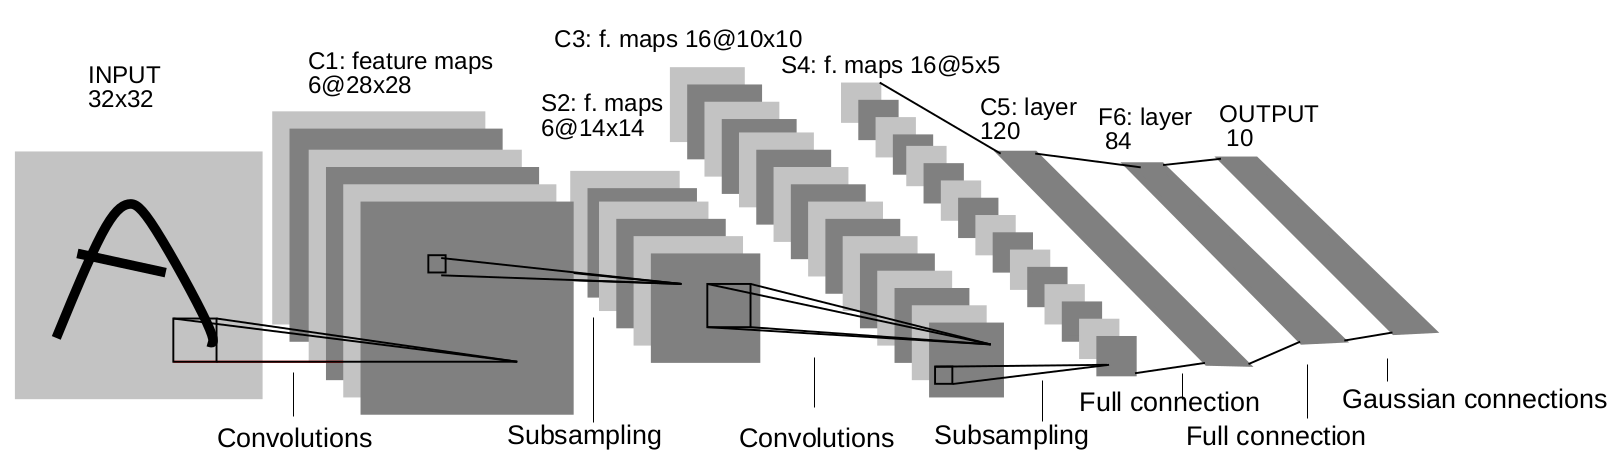
\includegraphics[scale=0.25]{imagenes/lenet}
            \caption[Red neuronal convolucional para la clasificación de dígitos manuscritos]{Red neuronal convolucional para la clasificación de dígitos manuscritos\\ Fuente: \citep{lecun-gradientbased-learning-applied-1998}}
        \end{figure}
        % \vspace{-8mm}
        % \begin{center}
        %     Fuente: \citep{lecun-gradientbased-learning-applied-1998}
        % \end{center}
        
        \subsubsection{STRIDES}
        Cuando se desea optimizar la operación sacrificando representabilidad o disminuir la muestra, se puede incrementar el tamaño del salto de la ventana deslizante al convolucionar la imágen con el filtro, a este salto se le llama \textbf{stride}
        
        
        Aplicando esta idea, se obtiene una fórmula general para calcular la dimensión de la matriz resultante al aplicar cada uno de los filtros con un stride $s$
        
        $$\frac{I_{alto} - k + s}{s} \times \frac{I_{ancho} - k + s}{s}$$ 
        
        \begin{figure}[H]
            \centering
            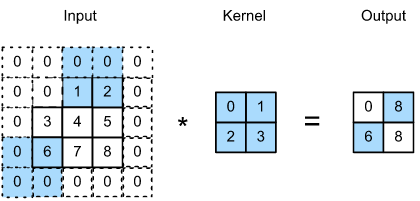
\includegraphics[scale=0.55]{imagenes/stride}
            \caption[Convolución con $s=2$]{Convolución con $s=2$\\ Fuente: \citep{zhang2020dive}}
        \end{figure}
        % \vspace{-8mm}
        % \begin{center}
        %     Fuente: \citep{zhang2020dive}
        % \end{center}
        \subsubsection{POOLING}
        Es una operación sobre la entrada bidimensional que con un stride $s$ recorre una ventana deslizante de dimensión $p \times p$ extrayendo información característica de cada sección de la entrada.
        
        Existen dos tipos de pooling más comunes, average pooling que promedia los valores activados en cada sección de la imágen sobre la que pasa la ventana y max pooling, el cual extrae el elemento más representativo, es decir el con mayor valor, de cada sección de la imágen.
        
        \begin{figure}[H]
            \centering
            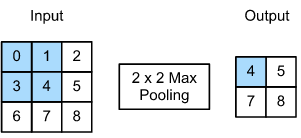
\includegraphics[scale=0.6]{imagenes/pooling}
            \caption[Pooling con con $s=1$]{pooling con con $s=1$\\ Fuente: \citep{zhang2020dive}}
        \end{figure}
        
        \subsubsection{MOBILENET V2}
        	Muchas tareas de aprendizaje profundo se despliegan en dispositivos con poco poder de cómputo, las redes neuronales con mejores resultados tienden a tener cada vez más capas y ser más costosas de computar, es por eso que nacen alternativas como la MobileNet, pensada para ejecutarse en dispositivos móviles y embedidos, sacrificando exactitud de predicción por velocidad, aún así obteniendo buenos resultados.
        	
        	La idea principal, es separar las convoluciones en dos etapas, la primera etapa llamada DepthWise Convolution, consiste en convolucionar la entrada de dimensiones $h_i\times w_i\times c$ con $c$ filtros de dimensiones $k\times k$, para obtener una salida de dimensiones $h_o\times w_o\times c$. La segunda etapa llamada PointWise Convolution recibe la salida de la DepthWise Convolution y le aplica $d$ filtros de dimensiones $1\times 1\times c$, para apilar las salidas y obtener finalmente una salida $h_o\times w_o\times d$.
        	
        	Este mismo resultado se puede obtener mediante una convolución con profundidad por definición, aplicando $d$ filtros de dimensión $k\times k\times c$, sin embargo el número de operaciones es mayor, ya que se realizan $h_i\cdot w_i\cdot c\cdot k^2\cdot d$ operaciones, comparadas con  las $h_i\cdot w_i\cdot c\cdot k^2 + h_o\cdot w_o\cdot c\cdot 1^2\cdot d$ de la mobilenet. En el caso de que la entrada tenga el mismo alto y ancho que la salida, $h\cdot w\cdot c\cdot(k^2 + d)$ operaciones de las convoluciones separables de la MobileNet.
        	
        	\begin{figure}[H]
        		\centering
        		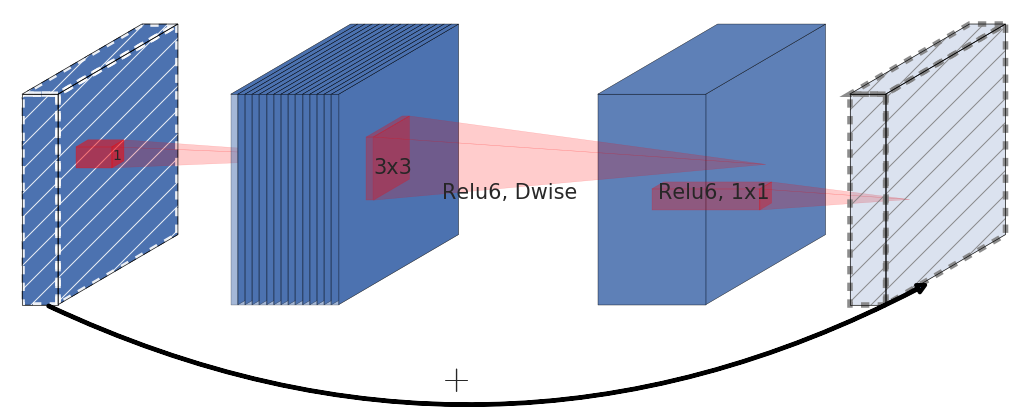
\includegraphics[scale=0.25]{imagenes/bottleneck}
        		\caption[Cuello de botella residual]{cuello de botella residual (residual bottleneck) Fuente:\citep{8578572}}
        		\label{bottleneck}
        	\end{figure}
        	
        	En base esta nueva convolución, se proponen bloques denominados cuellos de botella residuales detallados en la figura \ref{bottleneck}, que consisten en una capa PointWise con no linealidad Relu truncada con valor máximo 6 llamada Relu6 para obtener $t\cdot k$ filtros (con $t$ llamado el factor de expansión y $k$ la dimensión del filtro $k\cdot k$), seguido de una capa DepthWise $3\times3$ con stride $s$ y Relu6, para pasar por otra capa PointWise sin activación no lineal y que devuelve $d$ filtros. El término residual se refiere a que existe una conexión extra que envía directamente la salida de la primera PointWise Convolution a la última para sumarse de manera ponderada, con el fin de prevenir el desvanecimiento de los gradientes durante el entrenamiento \citep{8578572}.
        	
        
        	Usando estos bloques, se construye la arquitectura MobilenetV2 descrita en la tabla \ref{mobilenet2}
        	
        	\begin{center}
        		\footnotesize
        		\begin{tabular}{|c|c|c|c|c|c|}
        			\hline
					Entrada & Operador & Factor $t$ & Canales $c$ & Repeticiones $n$ & Stride $s$\\
					\hline
					$224^2\times3$ & conv2d & - & 32 & 1 & 2\\
					$112^2\times32$ & bottleneck & 1 & 16 & 1 & 1\\
					$112^2\times16$ & bottleneck & 6 & 24 & 2 & 2\\
					$56^2\times24$ & bottleneck & 6 & 32 & 3 & 2\\
					$28^2\times32$ & bottleneck & 6 & 64 & 4 & 2\\
					$14^2\times64$ & bottleneck & 6 & 96 & 3 & 1\\
					$14^2\times96$ & bottleneck & 6 & 160 & 3 & 2\\
					$7^2\times160$ & bottleneck & 6 & 320 & 1 & 1\\
					$7^2\times320$ & conv2d $1\times1$ & - & 1280 & 1 & 1\\
					$7^2\times1280$ & average pooling $7\times7$ & - & - & 1 & -\\
					$1^2\times1280$ & conv2d $1\times1$ & - & \#clases & - & -\\
        			\hline
        		\end{tabular}
        		\captionof{table}[MobileNet V2]{MobileNet V2 Fuente:\citep{8578572}}\label{mobilenet2}
        	\end{center}
        \subsubsection{FAST DEPTH}
        	Una de las áreas abiertas de investigación mediante redes neuronales convolucionales es la de inferencia de profundidad dada una imagen. A diferencia de los métodos de visión estéreo que mediante dos cámaras permite estimar la distancia de objetos al observador, esta tarea pretende hacerlo con una sola cámara, para esto se requiere de una arquitectura Encoder-Decoder, es decir una red codificadora que reciba la imagen RGB como entrada y extraiga las características más importantes de esta en un vector, luego otra red decodificadora, recibe como entrada este vector y devuelve la como salida una nueva imagen dependiendo de la tarea a resolver.
        	
        	Normalmente para este tipo de problemas se usan redes complejas con alto poder de abstracción, sin embargo para tareas con limitado poder de cómputo se debe simplificar la arquitectura, es así que nace la idea de la red FastDepth una red convolucional de código libre disponible en el repositorio de github de los autores \citep{icra_2019_fastdepth}.
        	
        	Esta red propone usar una mobilenet v1 como encoder y una nueva red decoder de 5 capas, este decodificador aplica una convolución DepthWise con bordes de relleno para obtener el mismo tamaño de salida, y PointWise para los filtros nuevos, luego de cada convolución se realiza una interpolación por vecinos más cercanos para duplicar el tamaño, hasta llegar a la última capa dónde se aplica solamente una convolicion PointWise.
        	
        	\begin{figure}[H]
        		\centering
        		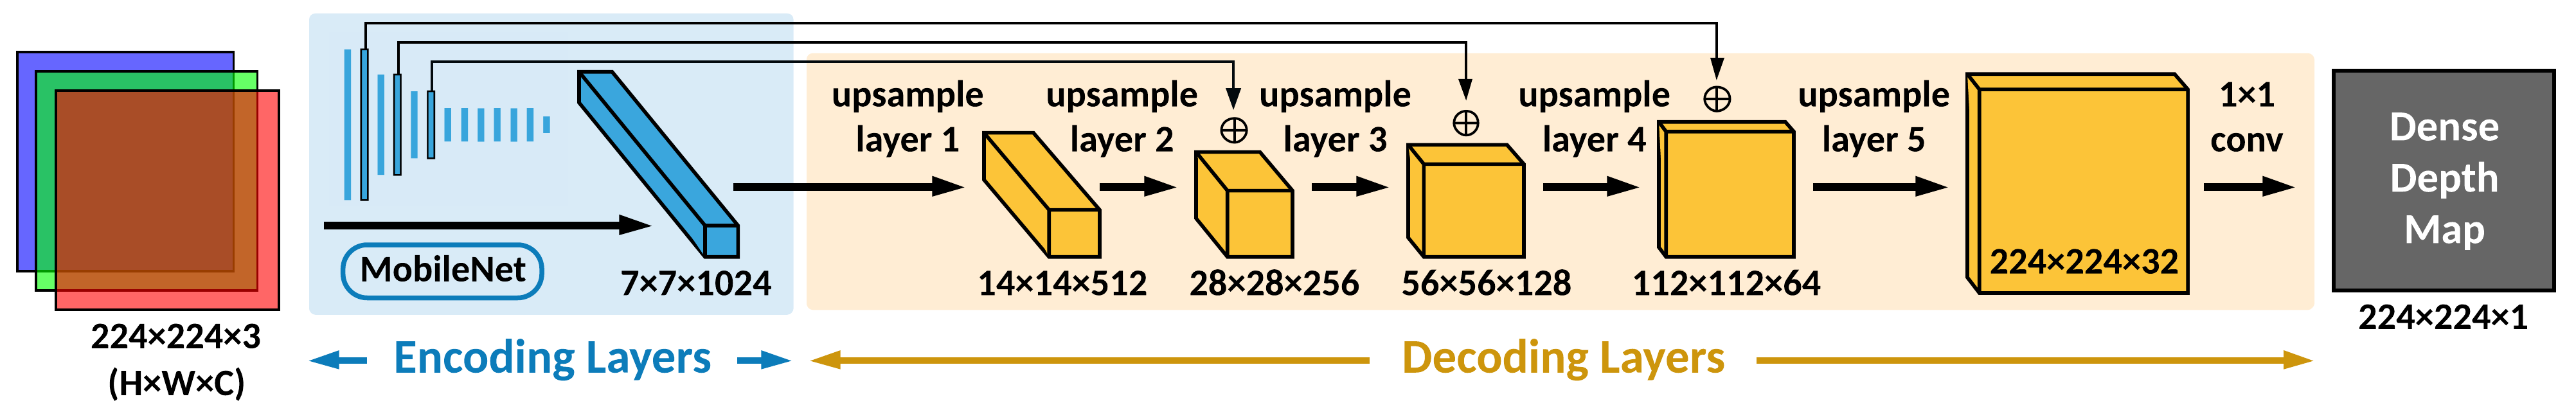
\includegraphics[scale=0.11]{imagenes/fastdepth}
        		\caption[Arquitectura FastDepth]{arquitectura FastDepth\\ Fuente: \citep{icra_2019_fastdepth}}\label{fastdepth}
        	\end{figure}
        	
        	La salida de esta red es una matriz de $224\times224$ con las estimaciones de distancia para cada píxel RGB de entrada.
        	
        	Como especifica la figura \ref{fastdepth} se tienen también conexiones residuales, o skip connections, que similar a los bloques de la mobilenet v2, permiten realizar saltos entre las conexiones de las capas mediante una suma ponderada a la capa resultante para así prevenir gradientes ceros durante el entrenamiento, debido a la forma de U de estas conexiones, a esta arquitectura se la denomina U-Net.
    \subsection{APRENDIZAJE DE REPRESENTACIONES PROFUNDAS}
	    En cada etapa de la red neuronal se extraen características representativas de la imagen que ayuden a realizar la predicción de la tarea para la cual se la entrena, conforme pasan más etapas en la red los filtros buscan características más específicas \citep{Goodfellow-et-al-2016}
	    
	    \begin{figure}[H]
 	        \centering
 	        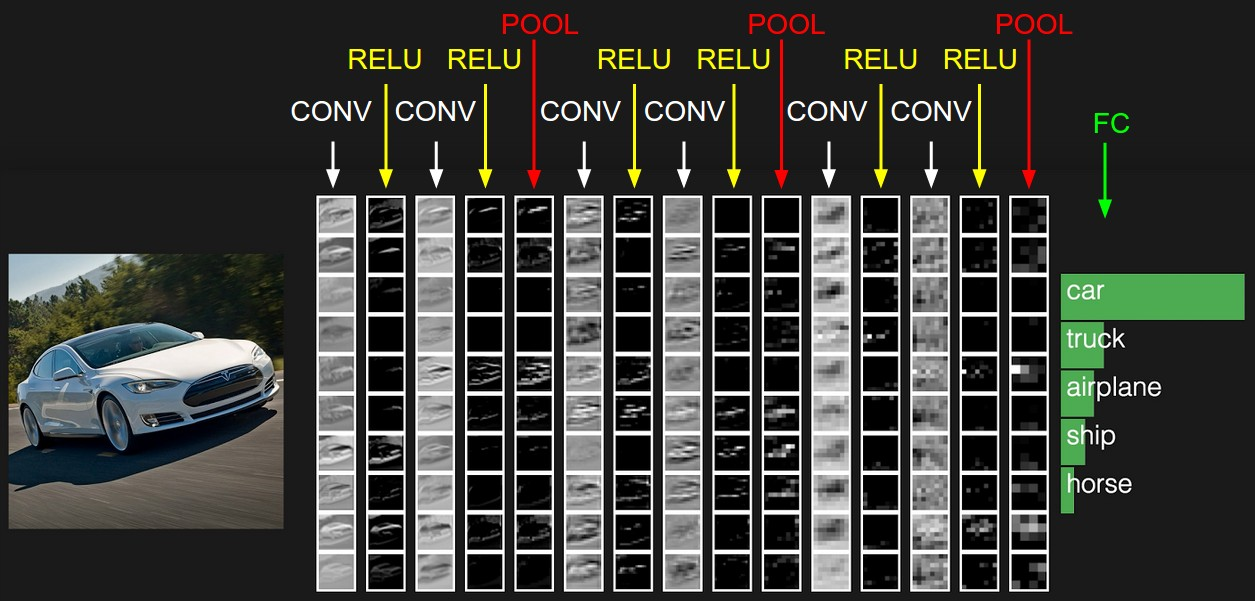
\includegraphics[scale=0.23]{imagenes/convnet}
 		    \caption[Extracción de las características profundas aprendidas]{Extracción de las características profundas aprendidas\\ Fuente: \citep{stanford_2020}}
	    \end{figure}

	    
	    \noindent de esta manera activando (dando valores altos) a ciertas partes de la imagen que es donde ``presta atención'' en busca de los objetos que desee clasificar o en base a los que predecir algún valor numérico, a esto se le llama aprendizaje de representaciones profundas, porque los filtros aprenden información desde bajo a alto nivel que caracterice los objetos en las etiquetas de entrenamiento.
		
		\begin{figure}[H]
			\centering
			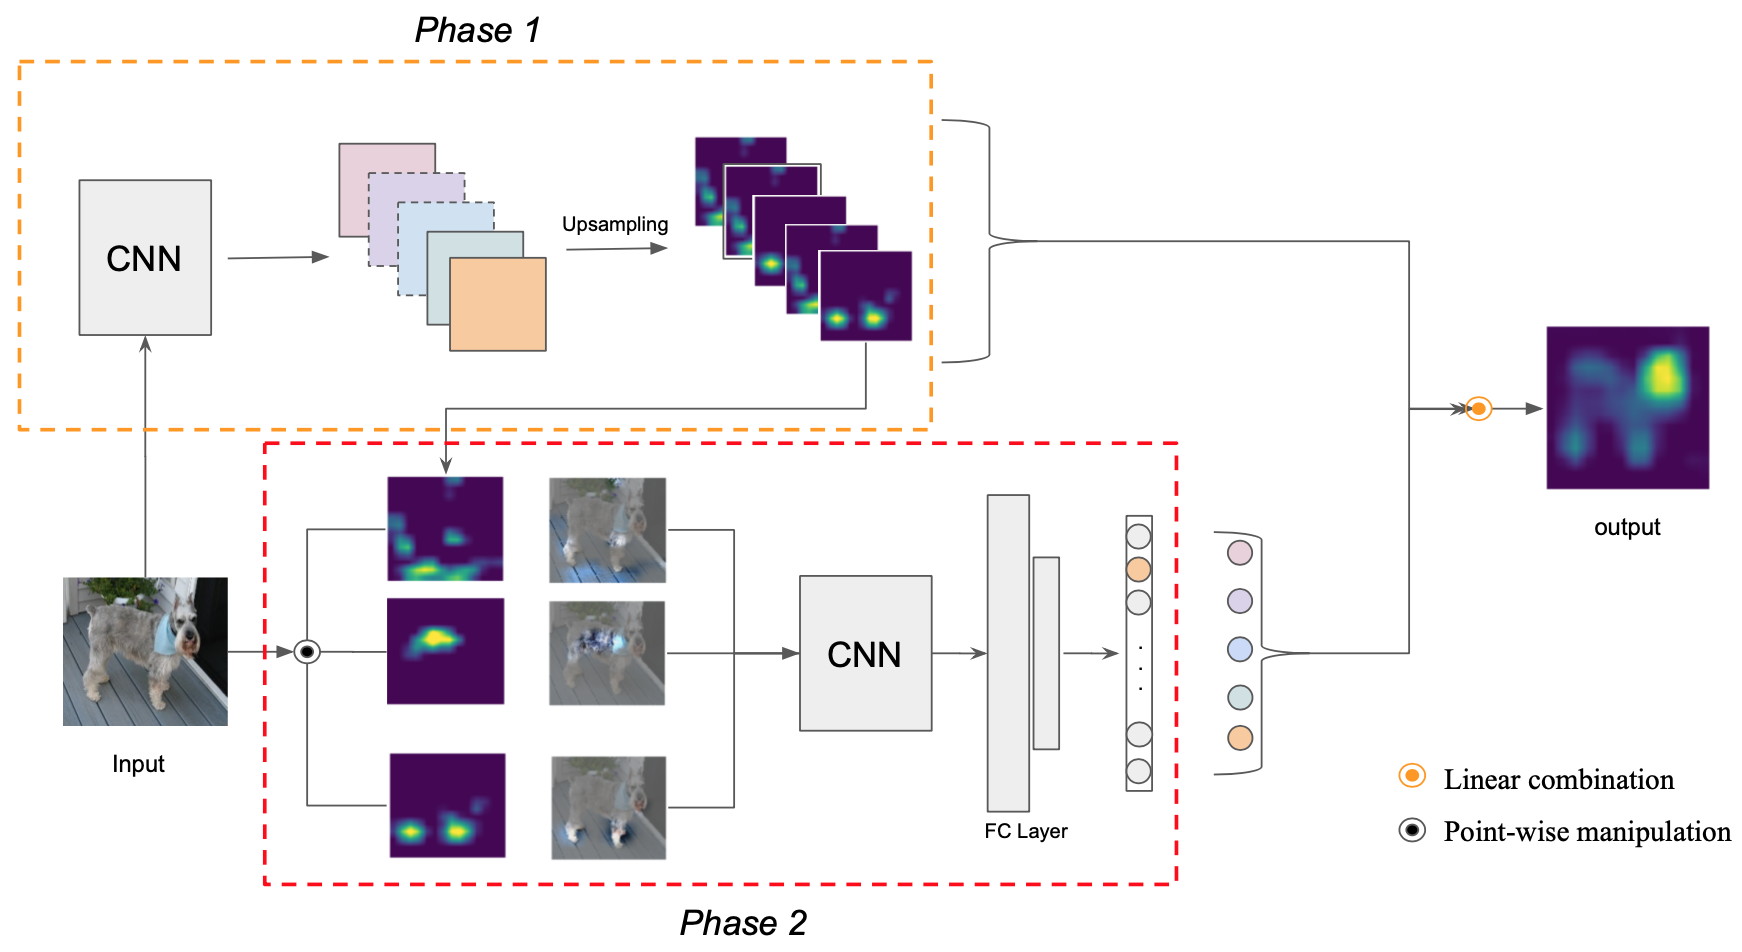
\includegraphics[scale=0.25]{imagenes/scorecam_net}
			\caption[Algoritmo ScoreCam]{algoritmo ScoreCam\\Fuente:\citep{Wang_2020_CVPR_Workshops}}\label{scorecam}
		\end{figure} 
		
		Uno de los algoritmos utilizados para esta tarea es ScoreCam, el cual calcula un mapa de prominencia dadas las capas activadas al evaluar una imagen por toda la red descrita en la figura \ref{scorecam}. Para lograrlo primero pasa la imagen por la red e intercepta la salida de la última capa convolucional, iterando por sus filtros. En cada iteración para el filtro i-ésimo, realiza un cambio de tamaño mediante interpolación para que el filtro tenga las mismas dimensiones de la imagen original, luego normaliza sus valores activados y los multiplica por la imagen original para re ingresar a la red, se captura la salida de la clase deseada y se acumula ponderando por la clase los valores del filtro por iteración, para finalmente realizar un cambio de tamaño a la variable acumulada y combinar con la imagen original para poder visualizar las áreas de interés de la imagen para la red.
	
	\section{MÉTRICAS DE ERROR}
\subsection{ERROR CUADRÁTICO MEDIO}
Al calcular la diferencia entre observaciones, es útil ponderar las distancias más grandes por sobre las distancias pequeñas, así se define el error cuadrático medio como:

\begin{equation}
	MSE = \frac{1}{n}\sum_{i=1}^n (\hat{y} - y)^2
\end{equation}

Ya que esta métrica se usa al comparar estimaciones y sus valores reales esperados, se denota por $\hat{y}$ a la predicción y $y$ al valor real \citep{hastie01statisticallearning}.

\subsection{ERROR ABSOLUTO MEDIO}
Debido a que el error cuadrático medio pondera de manera distinta cada diferencia, si bien es útil para minimizar errores de ajuste de modelos, es difícil de interpretar al reportar resultados, para esto se utiliza el error absoluto medio, también conocido como la media de la norma $\ell_1$, definido como:

\begin{equation}
	MAE = \frac{1}{n}\sum_{i=1}^n |\hat{y} - y|
\end{equation}

Esta función también se utiliza para ajustar modelos, sin embargo debido a la singularidad en el punto $0$, no es diferenciable en su dominio, por lo que dependiendo de la implementación se define una derivada en ese punto \citep{hastie01statisticallearning}.

\subsection{PRECISIÓN Y EXHAUSTIVIDAD}
% Con valor F
Cuando en tareas de clasificación se tienen conjuntos de datos desbalanceados, un cálculo de probabilidad de exactitud no es representativo del rendimiento real del modelo, por lo que se aplican la precisión y exhaustividad.

La precisión ($P$) se define como el número de positivos reales ($T_p$), dividido entre el total de verdaderos y falsos positivos $F_p$.

\begin{equation}
	P = \frac{T_p}{T_p + F_p}
\end{equation}

Una alta precisión indica que el umbral de clasificación es más estricto, por lo que pocos valores positivos se clasifican como tal, sin embargo los clasificados como positivo tienen una probabilidad alta de ser predicciones correctas.

La exhaustividad ($R$) se define como el número de positivos reales, dividido entre la suma de verdaderos casos positivos y falsos negativos ($F_n$).

\begin{equation}
	R = \frac{T_p}{T_p + F_n}
\end{equation}

Una alta exhaustividad o recall, significa que el umbral de clasificación es más permisivo, sin embargo, debido a esto muchas de las predicciones positivas, son en realidad negativas, teniendo así un alto índice de falsos positivos.

Una forma de representar estas dos métricas como una sola es mediante el valor F, definido como:

\begin{equation}
	F = 2\frac{P\cdot R}{P+R}
\end{equation}

al ponderar de manera equitativa la precisión y exhaustividad, un alto valor indica que ambas son altas por igual \citep{bishop}.

\subsection{ÍNDICE JACCARD}
El índice Jaccard, conocido también como intersección sobre unión, es un estadístico usado para medir la similaridad entre conjuntos finitos mediante una "superposición" de valores comunes.

Se define mediante la fórmula:

\begin{equation}
	IoU = \frac{|y\cap\hat{y}|}{|y\cup\hat{y}|}
\end{equation}

En tareas de segmentación semántica, este índice calcula la proporción de píxeles en común entre la máscara real y la estimada, y todos los píxeles que componen la combinación de ambas máscaras \citep{Goodfellow-et-al-2016}.
	
	\section{COMPILACIÓN EN TIEMPO DE EJECUCIÓN}
	Debido a que Python es un lenguaje lento por ser interpretado, en ocasiones donde se requiera código que se ejecture rápidamente sin cambiar de lenguaje, se recurre a la compilación justo a tiempo o Just in Time Compilation, la cual permite compilar una función con los argumentos recibidos la primera vez que se utiliza.
	
	Numba es una librería de código abierto que dota de esta funcionalidad a Python, compilando a código máquina a través de LLVM funciones que cumplan las restricciones para poder inferir correctamente el tipo de dato, está pensado para que de manera directa sólo sea necesario agregar el decorador @njit antes de alguna función para que sea compilada la primera vez que se use \citep{numba}.
	
	%\pospacechap
\chapter{MARCO APLICATIVO}
	\negspacesec
	\section{COMPRENSIÓN DEL PROYECTO}
En el presente trabajo se pretende lograr la conducción autónoma básica de un vehículo, al requerir ejecutar pruebas y análisis de resultados, debido a las limitaciones de no contar con el acceso a un vehículo con sensores en la vida real, se hace uso de entorno virtual en un simulador, el elegido para este trabajo es CARLA.

Como primer paso se deben definir los requerimientos, ya que la base de las predicciones son modelos estadísticos basados en datos se tiene la siguiente lista:

\begin{itemize}[nosep]
	\item Módulo de extracción de datos.
	\item Módulo de procesamiento de datos.
	\item Definir las arquitecturas de redes neuronales a utilizar para cada una de las tareas.
	\item Módulo de entrenamiento y evaluación.
	\item Visualización y análisis de las predicciones.
\end{itemize}

Una vez se tengan los datos a disposición, se tiene como objetivo entrenar las redes neuronales en tres tareas de inferencia:

\begin{itemize}[nosep]
	\item Aceleración y giro.
	\item Profundidad.
	\item Segmentación semántica.
\end{itemize}

Utilizando las predicciones de la segmentación para detectar semáforos mediante los contornos, para analizar el color, al igual que las predicciones de distancia para evitar colisiones con otros vehículos.

\begin{figure}[H]
	\centering
	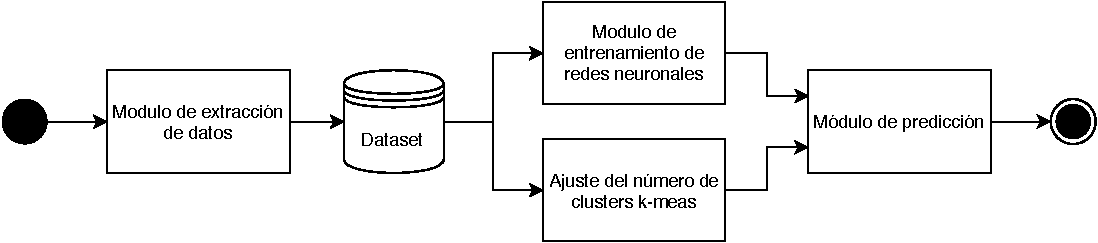
\includegraphics[scale=0.75]{imagenes/arquitectura_proyecto}
	\caption[Arquitectura del proyecto]{arquitectura del proyecto}
	\label{arquitectura_proyecto}
\end{figure}

Así la estructura del proyecto se resume en los componentes descritos en la figura \ref{arquitectura_proyecto}
	
	\pospacesec
	\section{COMPRENSIÓN DE LOS DATOS}
El simulador cuenta con un sistema integrado para el control de los vehículos llamado Traffic Manager, este hace uso de toda la información disponible sobre el mapa y los objetos en él, siendo estos la topología de las calles, distancia a los obstáculos y coordenadas de los demás vehículos, para mediante código configurar si se quiere ceder el control del vehículo al sistema o controlarlo nosotros.

Se implementa un módulo de extracción (figura \ref{extraccion}), que consiste en dejar que el sistema cree un vehículo denominado ``jugador'', que será con el que se trabaja, en alguna posición aleatoria del mapa, dejando que el sistema tome control conduciendo el vehículo mediante caminos arbitrarios durante un tiempo definido por 8000 fotogramas, generando datos en forma de imágenes y sus correspondientes etiquetas

\begin{figure}[H]
	\centering
	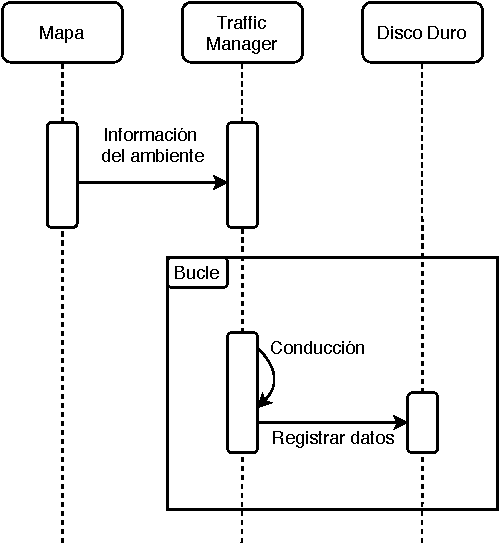
\includegraphics[scale=0.9]{imagenes/arquitectura-extraccion}
	\caption[Diagrama de secuencia de extracción de datos]{Diagrama de secuencia de extracción de datos}
	\label{extraccion}
\end{figure}

estas son de tres tipos.

\subsection{ACELERADOR Y DIRECCIÓN}
Es un par de números, el valor del acelerador en un rango $(0, 1)$, indica cuánto por ciento del acelerador está siendo presionado, la dirección es un valor entre $(-1, 1)$, equivalente a dos proporciones en una variable, indicando cuánto se debe girar a la izquierda o a la derecha.

\subsection{PROFUNDIDAD}
CARLA cuenta con una cámara virtual que codifica la profundidad o distancia a objetos en un fotograma, estos valores están codificados como números de 24 bits en una imagen RGB que deben ser normalizados de la siguiente manera:

$$\text{distancia} = \frac{R + G\cdot256 + B\cdot256\cdot256}{256\cdot256\cdot256 - 1} \cdot 1000$$

para obtener las distancias entre 0 y 1000 metros.

\begin{figure}[H]
	\centering
	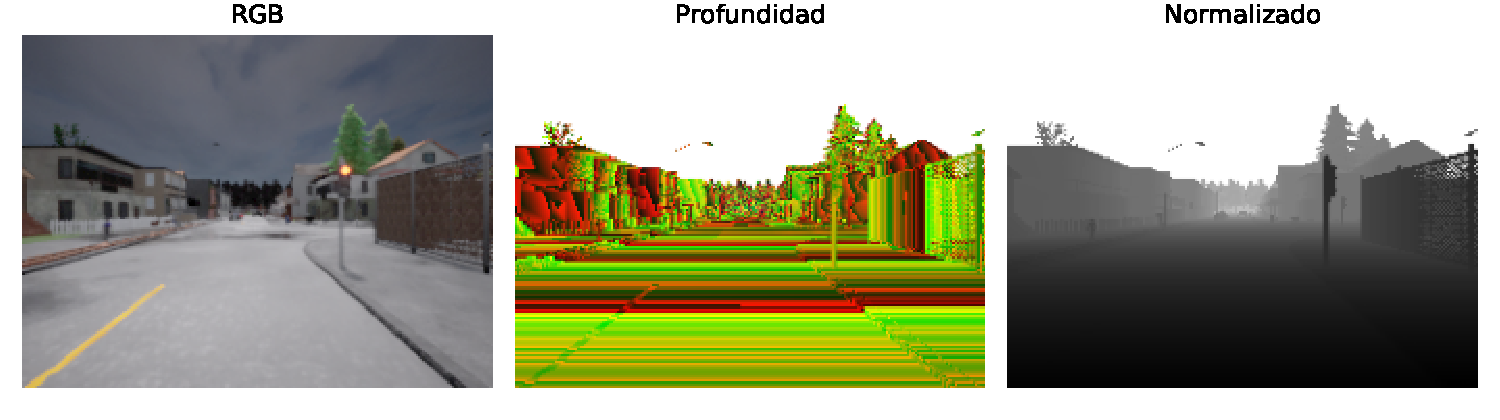
\includegraphics[scale=0.62]{imagenes/depth}
	\caption[Etiquetas de profundidad imagen]{Etiquetas de la profundidad de la imagen}
	\label{depth}
\end{figure}

\subsection{SEGMENTACIÓN SEMÁNTICA}
Igualmente CARLA cuenta con una cámara virtual que permite obtener la segmentación semántica de los objetos en un fotograma, estos datos están codificados como valores de píxeles en el canal rojo, cada valor de la máscara indica a qué clase pertenece el píxel correspondiente a esa coordenada de la imagen.

\begin{figure}[H]
	\centering
	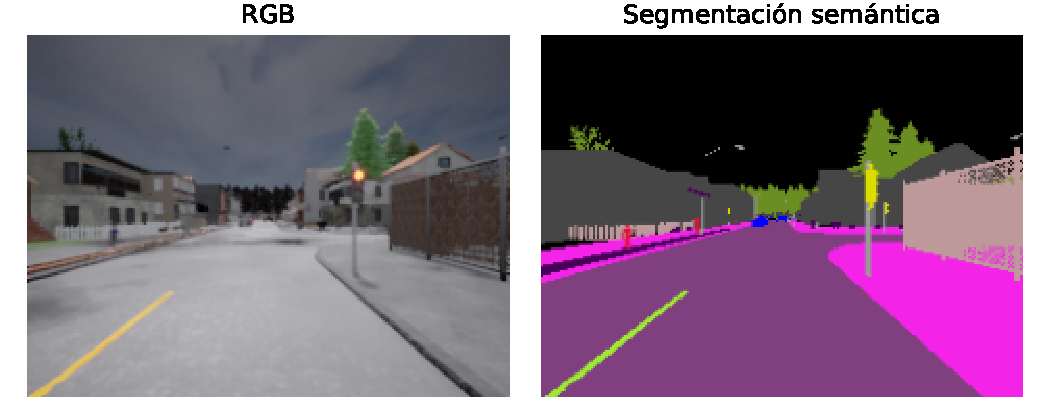
\includegraphics[scale=0.55]{imagenes/semseg}
	\caption[Segmentación semántica con códigos de color]{Segmentación semántica con códigos de color}
	\label{semseg}
\end{figure}

\begin{center}
	\footnotesize
	\begin{tabular}{|c|c|c|}
%	\begin{longtable}{|c|c|c|}
		\hline
		Valor mascara & Clase & Código de color\\
		\hline
		$0$ & Nada & \cellcolor{none}\\
		\hline
		$1$ & Edificios & \cellcolor{buildings}\\
		\hline
		$2$ & Cercas & \cellcolor{fences}\\
		\hline
		$3$ & Otro & \cellcolor{other}\\
		\hline
		$4$ & Peatones & \cellcolor{pedestrians}\\
		\hline
		$5$ & Postes & \cellcolor{poles}\\
		\hline
		$6$ & Lineas de carriles & \cellcolor{roadlines}\\
		\hline
		$7$ & Caminos & \cellcolor{roads}\\
		\hline
		$8$ & Aceras & \cellcolor{sidewalks}\\
		\hline
		$9$ & Vegetación & \cellcolor{vegetation}\\
		\hline
		$10$ & Vehículos & \cellcolor{vehicles}\\
		\hline
		$11$ & Paredes & \cellcolor{walls}\\
		\hline
		$12$ & Señales de transito & \cellcolor{trafficsigns}\\
		\hline
%	\end{longtable}
	\end{tabular}
	\captionof{table}[Correspondencia numérica de clases de segmentación]{Correspondencia numérica de las clases}\label{clases}
\end{center}

Para facilitar la visualización se aplica un código de color descrito por la tabla \ref{clases}, a las clases de píxeles en la imagen.

%\begin{figure}[H]
%	\centering
%	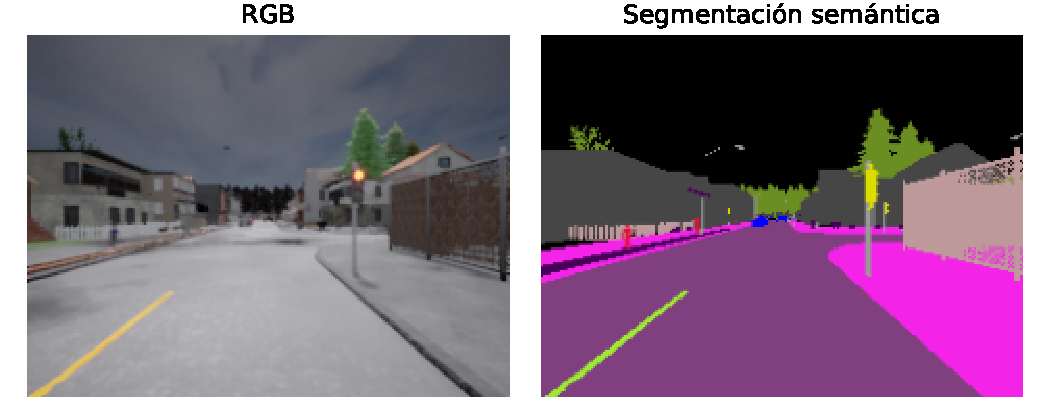
\includegraphics[scale=0.6]{imagenes/semseg}
%	\caption[Segmentación semántica con códigos de color]{Segmentación semántica con códigos de color}
%	\label{semseg}
%\end{figure}

Con el fin de simplificar el pre procesado de esta información, por cada simulación se genera una carpeta con tres imágenes dentro, una para imágenes estándar rgb que es lo que se observa a través de la cámara, una carpeta para las máscaras de la segmentación y una para las profundidades, cada archivo dentro de cada carpeta lleva el mismo nombre. Finalmente para las etiquetas del acelerador y dirección, se crea un archivo CSV que contenga la información de manera tabulada, con cada fila conteniendo las columnas

\begin{itemize}[nosep]
	\item throttle (acelerador): intensidad del acelerador.
	\item brake (freno): intensidad de freno.
	\item steer (aceleración): intensidad de dirección.
	\item junction (intersección): valor booleano sobre si la imagen pertenece o no a una intersección.
\end{itemize}

se tienen múltiples CSVs ya que se crean para cada simulación, y la información se obtiene del estado del vehículo y el mapa.
	
	% Primero se crea un dataframe centralizado
% Se ponen los junctions en carpetas Desktop/Codes/Tesis/NNTrain/Drive/Explore/junctions.ipynb ok
% Se etiquetan manualmente Documents/DriveDatasetStable/Train/junc_tag.py ok
%//train_dataset_junctions.csv o train_dataset.csv
% Se crea un dataframe final con los nuevos atributos Desktop/Codes/Tesis/NNTrain/Drive/Explore/unify_df.ipynb
% Se modifica la red de conducción
% Se entrena la red de conducción
% Copiar la implementación del fastdepth https://github.com/dwofk/fast-depth
% Se entrena la red de profundidad con un softmax 2D

\section{PREPARACIÓN DE DATOS}
	% Desktop/Codes/Tesis/DataExtraction/df_processing.ipynb
	Una vez recolectados los datos se debe empezar a procesarlos para agregar atributos de utilidad para los modelos y seleccionar la información que nos interesa, todas las etapas están implementadas en el lenguaje Python.
	
	\subsection{UNIÓN DE DATAFRAMES}
		Se debe unir los dataframes en formato CSV en un solo archivo para poder realizar futuras etapas de pre procesamiento.
		
		\inputminted[frame=lines,
		baselinestretch=1,
		fontsize=\footnotesize,
		autogobble]{python}{codigos/marco-aplicativo/df_processing.py}
		\captionof{listing}{unión de dataframes}
		
		Se cargan los dataframes en una lista, la cual luego se itera para crear una nueva columna en cada uno, esta columna contiene el nombre de los archivos referenciados en el dataframe bajo la estructura \textit{carpeta/archivo}, para luego unirlos en archivo mediante la función \textit{concat} de la librería de manipulación de datos \textit{pandas}.
		
	\subsection{ETIQUETADO DE INTERSECCIONES}
		Luego de un estudio de los datos obtenidos, se decide etiquetar las intersecciones agregando nuevos atributos:
		
		\begin{itemize}[nosep]
			\item path left: indica si se tiene un camino a la izquierda disponible.
			\item path right: indica si se tiene un camino a la derecha disponible. 
			\item path forward: indica si se tiene un camino recto disponible.
			\item action left: indica si el vehículo tomó el camino por izquierda.
			\item action right: indica si el vehículo tomó el camino por derecha.
			\item action forward: indica si el vehículo tomó el camino directo.
		\end{itemize}
	
		Para mantener la consistencia, a las imágenes que no pertenecen a ninguna intersección se les asignó la etiqueta \textit{no action} especificando que no se toma acción alguna.
		
		Debido a las características del mapa, que todas las intersecciones son de tipo T, se debe tener la información de qué caminos se tiene disponibles a tomar, con el fin de ingresar este dato en la etapa de inferencia.
		
		\begin{figure}[H]
			\centering
			\includegraphics[scale=1]{imagenes/arquitectura_juncs}
			\caption[Etapas del etiquetado de intersecciones]{etapas del etiquetado de intersecciones}
			\label{junctions}
		\end{figure}
		
		Este etiquetado se debe realizar de manera manual, por lo que primero se detectan los fotogramas que componen las intersecciones, para esto se extraen todas las imágenes marcadas como intersección, se procede a calcular la diferencia de índices entre imágenes, si la diferencia es mayor a 1 entonces inicia una nueva intersección, repitiendo este procedimiento se finaliza la etapa de separación en carpetas (figura \ref{junctions}), los archivos de cada carpeta tienen como nombre el id de simulación de origen, y el nombre de archivo original, para al unificar la información de nuevo sea fácil saber de dónde proviene cada intersección.
		
		Inmediatamente se implementa un script que lea carpeta por carpeta y muestre los fotogramas que componen cada intersección como vídeo, para que así el etiquetador pueda ingresar los atributos codificados para el tipo de intersección y la acción tomada, codificado con los controles de dirección estándar en un teclado (wasd).
		
		\inputminted[frame=lines,
		baselinestretch=1,
		fontsize=\footnotesize,
		autogobble]{python}{codigos/marco-aplicativo/junc_tag.py}
		\captionof{listing}{interfaz de etiquetado}
		
	\subsection{CONCATENACIÓN DE ATRIBUTOS}
		En la etapa final del pre procesamiento, se deben concatenar las nuevas columnas de atributos al CSV del conjunto de datos, llenando con valores positivos para la etiqueta \textit{no action} en caso de no pertenecer a una intersección, para esta tarea se implementa un script que cree una lista de valores para cada entrada con valor por defecto 1 y se van asignando ceros para cada elemento de las intersecciones en base a los nombres de los archivos en cada carpeta.
		
		Así finaliza la etapa de pre procesamiento de datos con un CSV indexando todas las imágenes recolectadas con sus correspondientes etiquetas de aceleración, dirección y caminos en intersecciones.
	
	\section{MODELADO}
	Una vez se tienen los datos disponibles, se debe definir una arquitectura de entrenamiento de modelos de aprendizaje profundo sobre los datos, las redes neuronales se implementan en Python usando la libreria Pytorch.
	
	\begin{figure}[H]
		\centering
		\includegraphics[scale=0.8]{imagenes/arquitectura_entrenamiento}
		\caption[Entrenamiento de tres redes neuronales]{entrenamiento de las tres redes neuronales}
		\label{training}
	\end{figure}
	
	Estos módulos están compuestos por tres redes neuronales basadas en la arquitectura Mobilenet V2, modificando la implementación estándar y su variante para inferencia de profundidad, un modelo estadístico llamado media exponencial móvil para el suavizado de la dirección, y el algoritmo K means para la cuantificación digital de colores.
	
	\subsection{RED DE CONDUCCIÓN}
		Denominada DriveNet, esta red es una modificación de la Mobilenet V2 estándar.
		
		\begin{figure}[H]
			\centering
			\includegraphics[scale=0.7]{imagenes/drivenet}
			\caption[Arquitectura DriveNet basada en Mobilenet V2]{Arquitectura DriveNet basada en Mobilenet V2}
			\label{drivenet}
		\end{figure}
	
		Se re define la sección del clasificador, en lugar de recibir los 1280 parámetros del extractor de características y predecir el número de clases, se convierte en una etapa de dos capas, una que recibe 1280 y exporta 251, a la que se le concatenan las 4 nuevas características, para enviar a la siguiente capa que recibirá 256 entradas y devuelve las 2 salidas finales, al adaptar la red a una tarea de regresión, el acelerador es un valor lineal entre 0 y 1, pero la dirección pasará por una tangente hiperbólica ($tanh(x)$) para mapear los valores entre $(-1, 1)$.
		
		\inputminted[frame=lines,
		baselinestretch=1,
		fontsize=\footnotesize,
		autogobble]{python}{codigos/marco-aplicativo/drivenet_capas.py}
		\captionof{listing}{definición de las capas de predicción}
		
		Como función de costo se usa el error cuadrático medio una para la aceleración y otra para la dirección, y la media de ambas como un costo conjunto denominado Joint MSE Loss.
		
		\inputminted[frame=lines,
		baselinestretch=1,
		fontsize=\footnotesize,
		autogobble]{python}{codigos/marco-aplicativo/drivenet_forward.py}
		\captionof{listing}{propagación hacia adelante y concatenación}
		
	\subsection{RED DE PROFUNDIDAD}
		Se usa la implementación de la red FastDepth sin modificaciones, basada en una MobilenetV2 con arquitectura de U-Net, los cambios que se dan son en la etapa de entrenamiento, ya que al ingresar las imágenes a la red, se trunca la distancia hasta máximo 30 metros, para simplificar la tarea de inferencia siendo que no es de interés centrarse en objetos a distancias mayores.
		
		\begin{figure}[H]
			\centering
			\includegraphics[scale=0.6]{imagenes/depthnet}
			\caption{Arquitectura FastDepth}
			\label{depthnet}
		\end{figure}
		
		\inputminted[frame=lines,
		baselinestretch=1,
		fontsize=\footnotesize,
		autogobble]{python}{codigos/marco-aplicativo/depthnet.py}
		\captionof{listing}{carga de la imagen para entrenamiento}
		
	\subsection{RED DE SEGMENTACIÓN SEMÁNTICA}
		Con el fin de simplificar las estructuras de los modelos, se utiliza la misma implementación de la red FastDepth modificando la función de costo por una Softmax 2D, ya que la tarea de segmentación semántica, es un tipo de clasificación píxel a píxel.
		
		\begin{figure}[H]
			\centering
			\includegraphics[scale=0.55]{imagenes/semsegnet}
			\caption{SemsegNet, FastDepth para clasificación 2D}
			\label{semsegnet}
		\end{figure}
		
	\subsection{SUAVIZADO DE DIRECCIÓN}
		Complementando las predicciones de las redes neuronales, se hace uso de una media exponencial móvil con parámetro $\alpha=0.7$, para suavizar las oscilaciones de la conducción con el fin de reducir ``volantazos'', tratando estos valores como una serie de tiempo.
		
		\begin{figure}[H]
			\centering
			\includegraphics[scale=0.4]{imagenes/ema}
			\caption[Aplicación de medias exponenciales móviles]{Aplicación de medias exponenciales móviles para suavizar la dirección}
			\label{ema}
		\end{figure}
	
		Este modelo se aplica en cada iteración de la simulación a las predicciones de giro sólo cuando los valores están dentro del rango $(-0.2, 0.2)$ y fuera de una intersección, ya que valores mayores de giro indican que el vehículo está tomando una curva y no generando una oscilación.
		
		\inputminted[frame=lines,
		baselinestretch=1,
		fontsize=\footnotesize,
		autogobble]{python}{codigos/marco-aplicativo/ema.py}
		\captionof{listing}{uso de media exponencial móvil en la predicción}
		
	\subsection{CAJA DELIMITADORA}
		Una vez se tiene la máscara de píxeles que componen los semáforos luego de la limpieza por dilatación, erosión y apertura, se aplica el algoritmo Flood Fill de manera iterativa, partiendo por los píxeles a partir de la coordenada 120 en dirección horizontal, así cada vez que se encuentre un valor positivo de la máscara, el algoritmo lo ``pintará'' de ceros eliminando el objeto pero devolviendo las coordenadas de los puntos extremos arriba-izquierda y abajo-derecha que definen el rectángulo de mínima área delimitando el objeto.
		
		\inputminted[frame=lines,
		baselinestretch=1,
		fontsize=\footnotesize,
		autogobble]{python}{codigos/marco-aplicativo/flood_fill.py}
		\captionof{listing}{Flood Fill para la extracción de la caja delimitadora}
		
		Debido a que Python es un lenguaje interpretado y lento para tareas pesadas se compila la función mediante numba con el decorador @JIT (Just in Time Compilation).
		
	\subsection{CUANTIFICACIÓN DIGITAL DEL COLOR}
		Aplicando K-Means se reduce la cantidad de colores en la imagen, manteniendo los más predominantes, al ingresar al algoritmo un recorte que contiene específicamente un semáforo, los 4 colores más predominantes serán los de la luz emitida, de esta manera, se analiza la existencia de píxeles con valores mayores a cero en ciertos canales.
		
		\begin{figure}[H]
			\centering
			\includegraphics[scale=0.65]{imagenes/sign}
			\caption[Cuantificación digital del color]{cuantificación digital del color para clasificación de semáforos}
			\label{semaforo}
		\end{figure}
		
		En caso que los canales rojo o rojo y verde tengan valores distintos de cero, se tienen rojo o amarillo en cuyo caso el semáforo está en estado de pare, si los valores son positvos en verde y azúl, se tiene alguna tonalidad de verde o blanco como se observa en la figura \ref{semaforo}
		
		\inputminted[frame=lines,
		baselinestretch=1,
		fontsize=\footnotesize,
		autogobble]{python}{codigos/marco-aplicativo/kmeans.py}
		\captionof{listing}{kmeans para clasificación del color de semáforos}
				
	\subsection{MODELO PARA LA CONDUCCIÓN AUTÓNOMA}
		Una vez descritos todos los módulos, se define el modelo y sus interacciones.
		
		La entrada será una imagen en RGB de resolución $240\times180$, la cual pasará por las tres redes descritas.
		
		\begin{figure}[H]
			\centering
			\includegraphics[scale=0.5]{imagenes/trapecio}
			\caption[Delimitado del área de interés para la detección de objetos]{trapecio delimitando el área de interés para la detección de obstáculos}
			\label{trapecio}
		\end{figure}
		
		Se usan las predicciones en conjunto de la DepthNet y SemsegNet, pasando previamente por una máscara que elimina todos los píxeles fuera de un trapecio (figura \ref{trapecio}) que corresponde al área de interés (con el fin de evitar falsos positivos), para extraer los píxeles correspondientes a posibles obstáculos, y se calcula la moda de las distancias redondeadas, para así decidir si existe peligro de colisión o no.
		
		\begin{figure}[H]
			\centering
			\includegraphics[scale=0.8]{imagenes/arquitectura_inferencia}
			\caption[Modelo de conducción autónoma]{modelo de conducción autónoma}
			\label{model}
		\end{figure}
		
		Se realiza un recorte a la zona donde se encuentre algún semáforo en caso de que se lo detecte, para lograr esta detección se aplica dilatación, erosión y apertura con el fin de reducir artefactos en las predicciones de la segmentación semántica, y se cuantiza el color para decidir si detenerse o no.
		
		Combinado con estas predicciones, la DriveNet infiere la dirección, la cual se suaviza mediante la media exponencial móvil, y aceleración, la cual se mantiene en caso de no presentarse obstáculos cerca ni semáforos en rojo.
		
		Los módulos descritos se pueden observar de manera estructurada en la figura \ref{model}.
	
	\section{EVALUACIÓN}
% Explicar el conjunto de validació cruzada
% Mostrar métricas de aprendizaje
% Listar resultados de predicción
% Mostrar los clusters encontrados por k means
% Justificar el uso de 4 clusters
Se analizan las curvas de aprendizaje para cada modelo usando Adam como optimizador.

\subsection{DRIVENET}
Para la red de conducción se tiene la curva dada en la figura \ref{drivenetcurve} de un total de 30 iteraciones, con parámetros $\alpha=0.001$, $\beta_1=0.9$, $\beta_2=0.999$. De estos resultados se decidió realizar pruebas entre la iteración 24 y 30, se tomaron los parámetros de la epoch 24 con errores cuadráticos medios de 0.00051 para el conjunto de entrenamiento y 0.00088 para el conjunto de validación.

\begin{figure}[H]
	\centering
	\includegraphics[scale=0.5]{imagenes/DriveNetCurve}
	\caption[Errores de entrenamiento y validación de la DriveNet]{errores de entrenamiento y validación de la DriveNet}
	\label{drivenetcurve}
\end{figure}

\subsection{DEPTHNET}
Para la red de profundidad se tiene la curva dada en la figura \ref{depthnetcurve} de un total de 24 iteraciones, con parámetros $\alpha=0.01$, $\beta_1=0.9$, $\beta_2=0.999$.

\begin{figure}[H]
	\centering
	\includegraphics[scale=0.5]{imagenes/DepthNetCurve}
	\caption[Errores de entrenamiento y validación de la DepthNet]{errores de entrenamiento y validación de la DepthNet}
	\label{depthnetcurve}
\end{figure}

De estos resultados se eligieron los parámetros de la iteración 20 con errores cuadráticos medios de 1.30575 para el conjunto de entrenamiento y 9.267 para el conjunto de validación.

Es importante notar que no se tomaron los parámetros de alguna iteración que distara poco del error de entrenamiento, sino de la iteración en la que se tenía el menor error de validación durante el entrenamiento.

\subsection{SEMSEGNET}
Para la red de segmentación semántica se tiene la curva dada en la figura \ref{semsegnetcurve} de un total de 7 iteraciones, ya que esta era la más costosa de computar, con los mismos parámetros que la DriveNet.

\begin{figure}[H]
	\centering
	\includegraphics[scale=0.5]{imagenes/SemsegNetCurve}
	\caption[Errores de entrenamiento y validación de la SemsegNet]{errores de entrenamiento y validación de la SemsegNet}
	\label{semsegnetcurve}
\end{figure}

De estos resultados se eligieron los parámetros de la iteración 7 con errores del tipo mean log softmax 2D de 0.08396 para el conjunto de entrenamiento y 0.09178 para el conjunto de validación.

Al igual que para la red de profundidad se eligieron los parámetros con el menor error en el conjunto de validación cruzada.

\subsection{CENTROIDES K-MEANS}
Finalmente se evalúa que la decisión sea correcta para el número de centroides en el algoritmo KMEans, debido a que el espacio de color RGB se puede representar como 3 dimensiones espaciales, se analizó gráficamente el desempeño del algoritmo, se decidió que 4 centroides era la mejor cantidad para la tarea de cuantificación digitalización del color.

Observando la figura \ref{colorspace}, se nota que de los cuatro centroides señalizados con figuras distintas de esferas y de color azul, dos de ellos están en el punto de mayor aglomeración que son los píxeles de colores oscuros del borde del semáforo, mientras que los otros dos están en los puntos más intensos del color rojo o verde y en el punto de combinación entre dos colores, blanco para el caso verde-azul y amarillo para rojo-verde.

\begin{figure}[H]
	\centering
	\includegraphics[scale=0.65]{imagenes/sign_3d}
	\caption[Espacios de color y centroides para dos semáforos distintos]{espacios de color y centroides para dos semáforos distintos}
	\label{colorspace}
\end{figure}
	
	\section{DESPLIEGUE}
	Para realizar el despliegue del proyecto se implementa un script que se comunique con el simulador para extraer imágenes desde una cámara virtual hasta que el usuario detenga el procedimiento, para cada iteración de la simulación se realizan las predicciones en base al modelo propuesto y se adicionan funciones de visualización de las predicciones de las redes.
	
	Los pasos más importantes son:
	\begin{enumerate}[nosep]
		\item Definir la pantalla de visualización de imágenes mediante la librería PyGame.
		\item Conectar con el simulador e inicializar el vehículo en el mapa con un clima aleatorio.
		\item Cargar los parámetros de las redes.
		\item Iniciar un bucle de iteraciones de la simulación a 30 fps.
		\item Detectar si se está en una intersección mediante el simulador y decidir al azar qué camino tomar.
		\item Ingresar los valores de entrada a cada red neuronal y recibir su salida.
		\item Corregir las oscilaciones con EMA.
		\item Si el vehículo no realiza alguna curva en intersección, se da un impulso mediante un acumulador de giro.
		\item Se procesan las predicciones de la segmentación semántica para las clases vehículos y postes.
		\item Se calcula la moda de las distancias de objetos cercanos.
		\item Se detecta la posición de los semáforos.
		\item Se predice un código de color, r para rojo o g para verde.
		\item Se usa el código de color para decidir si frenar o no.
		\item Se envían las decisiones finales de control al vehículo.
	\end{enumerate}
	
	el código del script está listado en el anexo $F.3$.
%	
%	
%	{\setstretch{1.0}
%	\begin{algorithm}[H]
%		\caption{\textit{Modelo de Conducción Autónoma}}
%		\SetAlgoLined
%		\KwData{$w:$ ancho de la imagen a mostrar}
%		\KwData{$h:$ alto de la imagen a mostrar}
%		\KwData{$drivepath:$ ubicación de los pesos de la DriveNet}
%		\KwData{$depthpath:$ ubicación de los pesos de la DepthNet}
%		\KwData{$semsegpath:$ ubicación de los pesos de la SemsegNet}
%		\vspace{2mm}
%		iniciar\_pygame($w$, $h$)\\
%		cliente $\leftarrow$ conectar\_carla()\\
%		mundo $\leftarrow$ conectar\_mundo()\\
%		jugador $\leftarrow$ iniciar\_jugador()\\
%		camara $\leftarrow$ crear\_cámara()\\
%		\vspace{2mm}
%		drive\_net $\leftarrow$ cargar($drivepath$)\\
%		depth\_net $\leftarrow$ cargar($depthpath$)\\
%		semseg\_net $\leftarrow$ cargar($semsegpath$)\\
%		\vspace{2mm}
%		ema $\leftarrow$ NULL\\
%		$\alpha$ $\leftarrow$ 0.75\\
%		giro $\leftarrow$ NULL\\
%		acelerador $\leftarrow$ NULL\\
%		freno $\leftarrow$ NULL\\
%		\While{$\infty$}{
%			img $\leftarrow$ obtener\_imagen(camara)
%			img $\leftarrow$ pre\_procesar\_imagen(img)
%			\tcc{obtener la posición y verificar si está en intersección}
%			posicion $\leftarrow$ obtener\_posicion()
%			accion $\leftarrow$ tomar\_accion(posicion)
%			\tcc{predecir}
%			acelerador, giro $\leftarrow$ drive\_net(img)
%			distancias $\leftarrow$ depth\_net(img)
%			segmentacion $\leftarrow$ semseg\_net(img)
%			
%			obstaculos $\leftarrow$ mascaras(segmentacion)
%			obstaculos\_d $\leftarrow$ dist\_obstaculos(obstaculos, segmentación)
%			
%			distancia $\leftarrow$ calcular\_moda(obstaculos\_d)
%			
%			ema $\leftarrow$ estabilizar\_direccion(ema, giro)
%			
%			semaforos $\leftarrow$ rectangulos\_flood\_fill(semaforos)
%			
%		}
%		
%	\end{algorithm}
	
	%\negspacechap
\chapter{RESULTADOS Y ANÁLISIS}
	\negspacesec
	%\section{Métricas de error}
\section{RENDIMIENTO DE LOS MÓDULOS} \label{metricas-error}
Al entrenar las redes neuronales, se siguió el procedimiento estándar de separar el conjunto de datos en entrenamiento y validación cruzada para analizar si el modelo está aprendiendo o memorizando los datos.

Así se seleccionan los parámetros de las iteraciones o epochs con menor error en el conjunto de validación cruzada, detallados en la tabla \ref{accuracies}, cuyas gráficas (figuras \ref{drivenetcurve}, \ref{depthnetcurve} y \ref{semsegnetcurve}) fueron descritas en la sección 3.5.

\begin{center}
	\footnotesize
	\begin{tabular}{|c|c|c|}
		\hline
		\textbf{Modelo} & \textbf{Error cuadrático medio} & \textbf{Iteración}\\
		\hline
		DriveNet & 0.00088 & 24\\
		\hline
		DepthNet & 9.267 & 20\\
		\hline
		SemsegNet & 0.09178 & 7\\
		\hline
	\end{tabular}
	\captionof{table}{Errores en el conjunto de validación de los parámetros seleccionados}\label{accuracies}
\end{center}

\subsection{ACELERACIÓN Y GIRO}
	Debido a que el error cuadrático medio penaliza de manera ponderada los valores más lejanos por sobre los cercanos, razón por la cual es una buena métrica de error a la hora de ajustar modelos, es difícil darle una interpretación comprensible al reportar resultados, es por eso que se calcula el error absoluto medio de las predicciones con los valores reales esperados del conjunto de validación.
	
	Para el caso de la predicción de aceleración, considerando que las redes no predicen el uso de frenos sino que estos se aplican cuando el modelo reacciona a semáforos u objetos cercanos, se obtiene un error absoluto medio de 0.067, es decir que la predicción de aceleración oscila $\pm 0.067$ de su valor real, esto debido a que la aceleración no es muy variable en el conjunto de datos de entrenamiento, por lo que al haber pocas situaciones inesperadas, las predicción es un número fijo con pocas variaciones en curvas.
	
	De manera similar para la dirección suavizada por la media exponencial móvil, se obtiene un error de $\pm 0.069$. Este error es mayor al de la aceleración, debido a que es más complicado para las redes mantener una dirección estable si no tiene información temporal, a pesar del uso de medias móviles exponenciales, esta no puede compensar todos los casos de variación.
	
	\begin{figure}[H]
		\centering
		\includegraphics[scale=0.3]{imagenes/preds/ema}
		\caption[Predicción Media Móvil Exponencial]{media móvil exponencial (rojo) suavizando los giros originales (azul)}
		\label{emapred}
	\end{figure}
	
	A pesar de las diferencias calculadas, el error es lo suficientemente pequeño para que no existan acelerones inesperados o giros que causen desestabilidad al vehículo, por lo que se consideraran errores aceptables en la práctica.
	
\subsection{ESTIMACIÓN DE PROFUNDIDAD}
	Al ser también una tarea de predicción de valores en $\mathbb{R}$, se calcula el error absoluto medio entre el mapa de profundidades estimado por la red y el del conjunto de datos de validación.
	
	En este caso el error es de $\pm 1.1931$, el cual es mucho más elevado que los errores de la red de conducción, esto debido a que las posibilidades de error son mayores ya que se predice la distancia pixel a pixel.

	La consecuencia de esto se nota mayormente al encontrarse con objetos cercanos, donde se puede predecir erróneamente que está muy cerca, en cuyo caso el vehículo se detiene totalmente ante un falso obstáculo, o el caso más peligroso que se da cuando el objeto está muy cerca y se predice que está una unidad más lejos del límite en el cual el modelo decide detener el auto y se produce una colisión.
	
	Gráficamente en la figura \ref{depthpred} se observa que la predicción es ``borrosa'' comparado con el mapa de profundidad original.
	
	\begin{figure}[H]
		\centering
		\includegraphics[scale=0.6]{imagenes/preds/depth}
		\caption[Predicción vs valor esperado de profundidad]{predicción vs valor esperado de profundidad}
		\label{depthpred}
	\end{figure}
	
\subsection{SEGMENTACIÓN SEMÁNTICA}
El módulo de segmentación semántica, considerando la limpieza de predicciones residuales mediante erosión, dilatación y apertura, es uno de los componentes más importantes, ya que la detención ante obstáculos y la detección de objetos depende de las predicciones de esta red, además, al ser una tarea de clasificación, se pueden analizar los resultados a mayor detalle con distintas métricas de error.
	\subsubsection{MATRIZ DE CONFUSIÓN}
	Se realiza el cálculo de la matriz de confusión, sin embargo, al existir muchas ocurrencias de cada clase, se decide estandarizar los valores a porcentajes por fila para mejor visualización, teniendo así la figura \ref{confussionmat}, dónde las diagonales indican los valores predichos correctamente, y fuera de la diagonal están las detecciones erróneas.
	
	\begin{figure}[H]
		\centering
		\includegraphics[scale=0.6]{imagenes/c_mat}
		\caption[Matriz de confusión de segmentación semántica]{matriz de confusión de segmentación semántica}
		\label{confussionmat}
	\end{figure}

	Se puede observar en la figura \ref{confussionmat}, que cuatro clases que se utilizan en la conducción, las cuales son peatones, postes, vehículos y señales de tránsito, tienen porcentajes de predicción de verdaderos positivos $48.25\%$, $54.04\%$, $92.54\%$ y $64.96\%$ respectivamente, siendo la detección de peatones y postes la menos exacta, la primera porque los peatones normalmente aparecen en aceras y en los bordes del campo de visión, y los postes debido a que son delgados y por la baja resolución de predicción es difícil para la red segmentarlos completamente.
	
	\subsubsection{PRECISIÓN Y EXHAUSTIVIDAD}
	Una vez se tiene la matriz de confusión, se pueden calcular la exactitud pixel a pixel, precisión, exhaustividad y el valor-F por clases, los cuales se listan en la tabla \ref{metricas}
	
%	Precision: Del total clasificado correctamente, cuánto porciento de estos son positivos.
%   Recall: Del total de los positivos, cuanto porciento son clasificados como positivos
	\begin{center}
		\footnotesize
		\begin{tabular}{|c|c|c|c|}
			\hline
			\textbf{Clase} & \textbf{Precisión} & \textbf{Exhaustividad} & \textbf{Valor-F}\\
			\hline
			Edificios  & 0.963 & 0.9738 & 0.9684\\
			\hline
			Cercas     & 0.8929 & 0.904 & 0.8984\\
			\hline
			Peatones   & 0.7141 & 0.4825 & 0.5759\\
			\hline
			Postes     & 0.7398 & 0.5404 & 0.6246\\
			\hline
			Carriles   & 0.0 & 0.0 & 0.0\\
			\hline
			Caminos    & 0.9855 & 0.9913 & 0.9884\\
			\hline
			Aceras     & 0.9517 & 0.9607 & 0.9562\\
			\hline
			Vegetación & 0.9218 & 0.9382 & 0.9299\\
			\hline
			Vehículos  & 0.9402 & 0.9254 & 0.9327\\
			\hline
			Paredes    & 0.8707 & 0.8936 & 0.882\\
			\hline
			Señales    & 0.7802 & 0.6496 & 0.7089\\
			\hline
		\end{tabular}
		\captionof{table}[Métricas de error de clasificación]{métricas de error de clasificación}\label{metricas}
	\end{center}

	De la tabla de errores y la matriz de confusión se puede notar primeramente que debido al desbalance de las muestras por clase, las predicciones de líneas de carriles son todas negativas, lo cual da una idea engañosa de alta exactitud, sin embargo el valor F, usado para compensar este sesgo dejan en claro que en realidad la predicción es totalmente errónea. Esto no es un problema para el modelo debido a que no se usa esta clase para las predicciones.
	
	Para las cuatro clases utilizadas tenemos que:
	\begin{itemize}
		\item \textbf{Peatones:} un $71.41\%$ del total de píxeles clasificados correctamente son positivos, $48.25\%$ de positivos reales son clasificados correctamente lo cual indica una alta cantidad de falsos negativos, con una exactitud balanceada de $57.59\%$.
		\item \textbf{Postes:} precisión $73.98\%$ y exhaustividad del $54.04\%$, dando menos falsos negativos con exactitud balanceada de $62.46\%$.
		\item \textbf{Vehículos:} precisión del $94.02\%$, exhaustividad de $92.54\%$ y exactitud de $93.27\%$ siendo esta la clase con los menores errores de predicción.
		\item \textbf{Señales de tránsito:} precisión $78.02\%$, exhaustividad $64.96\%$, con muchos menos falsos negativos, y $70.89\%$ de exactitud.
	\end{itemize}
	
	\begin{figure}[H]
		\centering
		\includegraphics[scale=0.6]{imagenes/preds/semseg}
		\caption[Predicción vs valor esperado de segmentación]{predicción vs valor esperado de segmentación}
		\label{semsegpred}
	\end{figure}
	
	Por estos resultados se puede afirmar que la detección de vehículos es la más exacta dando lugar a muy pocos casos en que no se los detecte para una parada efectiva. Por otra parte al detectar Peatones, Postes y Señales de tránsito en general, se tiene alta exhaustividad, es decir que si bien se detecta una cantidad considerable de píxeles de la clase, tiende a detectar menos píxeles de los que realmente componen al objeto (como se observa en la figura \ref{semsegpred}), sin embargo debido a la alta precisión, estos píxeles detectados tienen una alta confianza de ser de la clase predicha, en otras palabras, el modelo discrimina de manera agresiva, de forma que pocos valores pasan el umbral de clasificación, pero los que pasan tienen más seguridad de ser correctos.
	
	Una de las consecuencias de la alta exhaustividad, que se detallará en las pruebas del simulador, es que pueden no detectarse postes a tiempo dando lugar a colisiones.
	
	\subsubsection{CAJAS DELIMITADORAS}
	Finalmente, haciendo uso de las máscaras de segmentación por clase, se pueden visualizar las cajas delimitadoras de los objetos, haciendo uso del flood fill, para comprobar las predicciones gráficamente mediante un código de color para cada clase, celeste para vehículos, naranja para peatones, rosado para postes y rojo o verde para semáforos dependiendo de su estado.
	
	\begin{figure}[H]
		\centering
		\includegraphics[scale=0.64]{imagenes/preds/boxes}
		\caption[Cajas delimitadoras]{cajas delimitadoras}
		\label{boxes}
	\end{figure}

	en el caso de la figura \ref{boxes}, se observa que en la imagen b, no se detectó el semáforo, debido a que el área de la segmentación es muy pequeña para ser considerada una clasificación válida, de manera similar en la imagen c, sólo se detecta la parte de la luz del poste.
	
	\subsubsection{ÍNDICE JACCARD}
	Aplicando el índice de Jaccard, conocido como Intersection Over Union (IoU), otra métrica útil en la segmentación semántica, se obtiene la siguiente tabla de porcentajes:
	
	\begin{center}
		\footnotesize
		\begin{tabular}{|c|c|}
			\hline
			\textbf{Clase} & \textbf{IoU}\\
			\hline
			Edificios & 90.88\%\\
			\hline
			Cercas &  69.54\%\\
			\hline
			Peatones & 45.72\%\\
			\hline
			Postes & 31.93\%\\
			\hline
			Carriles & 03.52\%\\
			\hline
			Caminos & 97.55\%\\
			\hline
			Aceras & 91.01\%\\
			\hline
			Vegetación & 77.76\%\\
			\hline
			Vehículos & 72.46\%\\
			\hline
			Paredes & 57.26\%\\
			\hline
			Señales & 37.25\%\\
			\hline
		\end{tabular}
		\captionof{table}[Índice de Jaccard]{Índice de Jaccard de la segmentación semántica}\label{iou}
	\end{center}

	si se interpretan los valores como el porcentaje de superposición de la máscara real y la máscara predicha para cada clase, se observa que de las cuatro clases que más nos interesan los postes y señales de tránsito tienen los peores valores debido a la alta discriminación de píxeles de la red neuronal, mientras que los peatones y vehículos tienen mayor porcentaje, útil para evadirlos como obstáculos en la vía.
	
\subsection{DETECCIÓN Y CLASIFICACIÓN DE SEMÁFOROS}
	% Porcentaje de semáforos correctamente clasificados
	Debido a que el segmentador no discierne entre semáforos y las demás señales de tránsito, la clasificación de si lo es o no, y su color depende del módulo basado en K-means, evaluando la exactitud de este componente, se obtuvo que clasifica correctamente semáforos verdes en un $98.65\%$ de entre $1848$ pruebas, y rojos en un $99.52\%$ de exactitud de $2102$ imágenes. El $1.35\%$ de error en el color verde se da cuando se clasifican erroneamente semáforos amarillos que para la tarea se consideran igual a los rojos. Por otra parte el $0.48\%$ de error en semáforos rojo se debe al porcentaje de falsos negativos, es decir, la proporción de rojos reales clasificados como otro tipo de señal de tránsito. Así la exactitud total de clasificación de los colores es de $99.08\%$.
	
	\begin{figure}[H]
		\centering
%		\includegraphics[scale=0.65]{imagenes/preds/semaforos}
		\includegraphics[scale=0.58]{imagenes/preds/semaforos}
		\caption[Cuantización y Clasificación del Color]{cuantización y clasificación del color}
		\label{semaforos}
	\end{figure}
	
	% Semáforos con caja delimitadora
	Una vez calculado el error en la clasificación del color se puede visualizar en la figura \ref{semaforos} las predicciones del módulo. El color de la caja delimitadora indica la predicción, y a su lado se muestra la cuantización realizada por K-Means sobre la que se aplican los umbrales de clasificación.
	
% BACKUP TABLA
%\begin{center}
%	\footnotesize
%	\begin{tabular}{|c|c|c|c|c|}
%		\hline
%		\textbf{Clase} & \textbf{Exactitud} & \textbf{Precisión} & \textbf{Exhaustividad} & \textbf{Valor-F}\\
%		\hline
%		Edificios & 0.9874 & 0.963 & 0.9738 & 0.9684\\
%		\hline
%		Cercas    & 0.9963 & 0.8929 & 0.904 & 0.8984\\
%		\hline
%		Peatones  & 0.9991 & 0.7141 & 0.4825 & 0.5759\\
%		\hline
%		Postes    & 0.9951 & 0.7398 & 0.5404 & 0.6246\\
%		\hline
%		Carriles  & 0.9972 & 0.0 & 0.0 & 0.0\\
%		\hline
%		Caminos   & 0.9928 & 0.9855 & 0.9913 & 0.9884\\
%		\hline
%		Aceras    & 0.9907 & 0.9517 & 0.9607 & 0.9562\\
%		\hline
%		Vegetación& 0.9914 & 0.9218 & 0.9382 & 0.9299\\
%		\hline
%		Vehículos & 0.9962 & 0.9402 & 0.9254 & 0.9327\\
%		\hline
%		Paredes   & 0.9984 & 0.8707 & 0.8936 & 0.882\\
%		\hline
%		Señales   & 0.999 & 0.7802 & 0.6496 & 0.7089\\
%		\hline
%	\end{tabular}
%	\captionof{table}[Métricas de error de clasificación]{métricas de error de clasificación}\label{metricas}
%\end{center}
	
	\pospacesec
	\section{REPRESENTACIONES APRENDIDAS} \label{representaciones-aprendidas}
% Distancias en ROI
\subsection{DISTANCIAS EN LA REGIÓN DE INTERÉS}
Al combinar la máscara de segmentación de posibles obstáculos con el mapa de profundidades se simplifica la tarea de calcular la distancia a estos, además al considerar sólo el trapecio delimitando el área de circulación denominada región de interés, se reducen las falsas detecciones, como se puede observar en la figura \ref{distpred}

\begin{figure}[H]
	\centering
	\includegraphics[scale=0.65]{imagenes/preds/distance}
	\caption[Distancia a de objetos]{distancia a objetos en el área de interés}
	\label{distpred}
\end{figure}

en la primera fila se tienen las detecciones generales usando las máscaras de segmentación, en la segunda los mapas de profundidad, y en la tercera la distancia estimada solamente a los posibles obstáculos, esta distancia general se calcula mediante la moda del valor de los píxeles del mapa de profundidades, así en cuanto un objeto está cerca, la mayoría de sus píxeles tendrán un valor bajo, siendo el límite de 4 metros a partir de la cual se empieza a frenar.

\subsection{VISUALIZACIÓN DE ZONAS DE INTERÉS}
% ScoreCam
Con el fin de comprender gráficamente a qué partes de la imagen la red neuronal de conducción presta atención durante la predicción del giro, se aplica el algoritmo scorecam, del cual se obtiene un mapa de calor que une a la imagen original, y cuyos valores altos indican mayor atención en la región.

\begin{figure}[H]
	\centering
	\includegraphics[scale=0.6]{imagenes/preds/scorecam}
	\caption[Regiones de Interés en la Inferencia de Dirección]{regiones de interés en la inferencia de dirección}
	\label{scorecampred}
\end{figure}

En la figura \ref{scorecampred} se observan en los casos $a$ y $b$ que aparte de la atención en el asfalto, debido a que se comparten los filtros para la inferencia de aceleración, se fija en la acera derecha, mientras que en la imagen $c$, al no tener una acera en el lado esperado se centra en la que está al frente, en la nueva calle a incorporarse.
	
	\section{PRUEBAS EN SIMULADOR} \label{pruebas-simulador}
% rendimiento en simulacion (imágenes con giros y sus predicciones),
% gráfica del EMA.
% Casos de predicciones correctas vs erroneas en calles.
% Casos de predicciones correctas vs erroneas en intersecciones.
Una vez se tiene la certeza del funcionamiento del modelo mediante el análisis de sus métricas de error, se comprueban los resultados empíricamente con simulaciones en el ambiente virtual de la ciudad de CARLA.
\subsection{CONDUCCIÓN}
Ya se revisaron los resultados de segmentación, estimación de distancias y clasificación de objetos en la imagen, luego de pasar por todas las etapas descritas del modelo, las salidas obtenidas son el valor del giro y la aceleración.

\begin{figure}[H]
	\centering
	\includegraphics[scale=0.63]{imagenes/preds/steer}
	\caption[Comparación de Dirección Real y Estimada]{comparación de dirección real y estimada}
	\label{steer}
\end{figure}

Comparando las predicciones en distintas situaciones se tienen los resultados de la figura \ref{steer}, de la cual se puede observar en los casos $a, b, c, h, i$, los cuales consisten en giros durante intersecciones, que el modelo es mucho más agresivo al tomar las curvas, aplicando un giro mayor de la dirección. En el caso $f$ que es una intersección en la cual se decide seguir recto, predice correctamente no girar. En la situación de la imagen $g$, se tiene una casi colisión con otro vehículo, en cuyo caso la predicción es 0, al igual que la aceleración, y finalmente en las imágenes $d$ y $e$ no existe mucha variación del $0$ ya que se encuentra en una recta dentro de su carril.

\subsection{FALLOS}
A pesar del buen rendimiento del modelo en las situaciones de prueba, siempre existe un margen de error contemplado en las métricas evaluadas, así se presentan situaciones puntuales donde el vehículo se detiene abruptamente al confundir charcos de agua en la vía con vehículos cercanos (figura \ref{charco}), o los más graves cuando se sale del camino y colisiona con objetos en las aceras \ref{colision}.

\begin{figure}[H]
	\centering
	\includegraphics[scale=0.7]{imagenes/preds/err1}
	\caption[Charco erroneamente Clasificado]{Charco erroneamente Clasificado}
	\label{charco}
\end{figure}

%\begin{figure}[H]
%	\centering
%	\includegraphics[scale=0.6]{imagenes/preds/err2}
%	\caption[Colisión con Poste]{colisión con poste}
%	\label{colision}
%\end{figure}

En la figura \ref{colision} se nota que la segmentación falla al no detectar el poste como obstáculo lo cual deriva en que no se calcule la distancia a este y se produzca la colisión.

\begin{figure}[H]
	\centering
	\includegraphics[scale=0.22]{imagenes/preds/crash1}
\end{figure}

\begin{figure}[H]
	\centering
	\includegraphics[scale=0.22]{imagenes/preds/crash2}
	\caption[Colisión con Poste]{colisión con poste}
	\label{colision}
\end{figure}

En total se realizaron 17 simulaciones de prueba de las cuales en 3 se cometieron errores, los cuales fueron confundir un charco como vehículo, frenando totalmente y no reanudando la marcha,  el de salirse del camino sin detectar un poste, colisionando así contra él, y el de invadir un carril en contra ruta frenando para no colisionar y congestionando el tráfico ya que no puede dar marcha atrás.
	
	\section{PRUEBA DE LA HIPÓTESIS}
	
	Para la prueba de la hipótesis ``\textit{El modelo de conducción autónoma mediante el uso de aprendizaje profundo y algoritmos de visión computacional alcanza una autonomía de nivel 2 en vías de doble sentido con separación física.}'' se siguió los siguientes pasos.
	
	\begin{enumerate}[nosep]
		\item Se evaluaron los porcentajes de exactitud de predicción de las máscaras de segmentación y estimación de distancias a partir de las salidas de la DepthNet y SemsegNet (modelos de aprendizaje profundo).
		\item Se calculó el error de detección y clasificación del color de semáforos, aplicando Flood Fill para la detección de la caja delimitadora y K-Means para la clasificación del color (algoritmos de visión computacional).
		\item Se evaluó el error de la predicción de aceleración y frenado, en base a las predicciones conjuntas de las tres redes neuronales (DepthNet, SemsegNet y DriveNet) combinadas con la clasificación de los semáforos.
		\item Se obtuvo el error de estimación de dirección tanto a la izquierda como derecha en base a la predicción de la DriveNet.
	\end{enumerate}
	
	En base a los cálculos obtenidos se puede afirmar que:
	
	\begin{itemize}[nosep]
		\item Con un porcentaje de exactitud de clasificación para la detección de obstáculos y semáforos de un $71.41\%$, el error del control longitudinal es de $\pm 0.067$, considerando valores negativos como frenado y positivos como aceleración se obtiene un $6.7\%$ de error en el control longitudinal.
		\item El error de la dirección es de $\pm0.069$ lo que da lugar a un $6.9\%$ de error en el control lateral.
		\item De las 17 pruebas realizadas un $82\%$ son satisfactorias (3 pruebas con fallos).
	\end{itemize}

	Por lo tanto con un $93.2\%$ de confianza se puede afirmar que se obtiene una conducción autónoma de nivel 2 en el $82\%$ de las situaciones (17 pruebas).
		
	
	%\negspacechap
\chapter{CONCLUSIONES Y RECOMENDACIONES}
	\negspacesec
	\section{CONCLUSIONES}
Finalmente se concluye para cada objetivo específico
\begin{itemize}
	\item \textit{Diseñar un componente de aumentación y preprocesamiento de datos para extraer y crear un dataset con el fin de resolver la tarea.}
	
	Se diseñó un componente para, extraer imágenes y sus etiquetas de simulaciones, aumentar atributos con el fin de eliminar la ambigüedad en las intersecciones mediante una clasificación manual, y organizar las imágenes de cada simulación en su respectiva carpeta, indexado y etiquetado en un archivo csv.
	
	\item \textit{Reducir la complejidad de implementación del modelo mediante el uso de solamente una cámara.}
	
	Se redujo la complejidad de la implementación aplicando redes neuronales y algoritmos de visión artificial para inferir información extra a partir de una imagen RGB obtenida de una sola cámara, logrando así prescindir de sensores extra para la percepción del ambiente.
	
	\item \textit{Modificar y entrenar redes neuronales con una alta exactitud en las predicciones utilizando menos requisitos de cómputo.}
	
%	Se adaptó la red MobileNet para recibir como entrada extra la decisión en intersecciones, se cambió la función de costo de la red FastDepth para adaptarla a la tarea de clasificación bidimensional requerida en segmentación semántica, se entrenaron ambas redes en el conjunto de datos preparados para la tarea, además que se modificó la entrada de datos de la red FastDepth para que las predicciones tengan un límite de 30 metros, simplificando así la tarea con el fin de obtener mejores resultados, ya que todas las redes están pensadas para reducir requisitos computacionales sacrificando la complejidad de la distribución de datos que pueden ajustar, finalmente se analizó la exactitud mediante métricas de error descritas en la sección \ref{metricas-error}, obteniendo un buen resultado de predicción.
	
	Se modificaron y entrenaron las redes MobileNet y FastDepth para inferir la aceleración, dirección, profundidad y segmentación semántica, con menores requisitos computacionales al estar diseñadas para ejecutarse en dispositivos embedidos, obteniendo buenos resultados de predicción analizados en la sección \ref{metricas-error}.
	
	\item \textit{Analizar las predicciones de los modelos entrenados para comprobar si las representaciones aprendidas son invariantes a los cambios de perspectiva, iluminación y objetos en la imagen.}
	
%	Se exportaron las predicciones por fotograma de simulaciones aleatorias, así se analizó lo que predice cada red, el módulo de clasificación de semáforos, para comprobar que son invariantes a los cambios de iluminación en diferentes condiciones climáticas, a los objetos y las perspectivas en las que aparecen, segmentándolos y ubicándolos correctamente con un alto porcentaje de exactitud como se detalla en la sección \ref{representaciones-aprendidas}, y visualizando en la sección \ref{pruebas-simulador} las áreas de interés de la red neuronal al predecir la dirección, siendo lo más llamativo que busca la acera en el lado derecho para mantenerse en el carril.
	
	Se analizaron las predicciones fotograma por fotograma de simulaciones con diferentes condiciones climáticas, vehículos en distintas perspectivas y objetos de interés en distintas posiciones, se constató en las secciones \ref{representaciones-aprendidas} y \ref{pruebas-simulador} que los modelos y algoritmos con los parámetros elegidos son invariantes a estos cambios, además que se comprendió que la red de conducción basa su inferencia en la posición de la acera derecha en la imagen.
	
	\item \textit{Combinar las salidas de algoritmos de visión computacional y modelos de aprendizaje profundo para mejorar la generalización de predicciones.}
	
%	Se implementó un flujo de pasos que realiza un post procesamiento a las predicciones de las máscaras de segmentación de los objetos a detectar mediante dilatación, erosión y apertura para reducir las falsas predicciones, adicionalmente, se implementó un algoritmo de grafos para coloreado de imágenes, modificándolo para obtener el mínimo rectángulo que encierra un objeto en la máscara predicha por la SemsegNet, y finalmente se aplicó K-Means con umbrales de valores de píxeles para la clasificación de semáforos en las detecciones de señales de tránsito, además del color de estos, y así decidir si frenar o no de manera independiente a las predicciones de la red de conducción.
	
	Se combinaron las salidas de las redes neuronales de profundidad y segmentación semántica con las operaciones de dilatación, erosión y apertura, reduciendo así estimaciones residuales, además de la clasificación de semáforos por cuantización de colores para complementar las predicciones de aceleración por la red de conducción, logrando así generalizar las inferencias del acelerador y dirección dada la imagen de entrada.
	
	\item \textit{Probar el rendimiento del modelo en una simulación, analizando casos de fallas y qué situaciones puede manejar correctamente.}
	
%	Se realizaron simulaciones dónde el vehículo se condujo solo hasta que cometiera un error o excediera un tiempo límite sin errores, así se probó que en general el vehículo puede conducirse solo, cometiendo errores en situaciones puntuales, en base a estos resultados se concluye basándose en la tabla \ref{niveles}, que se obtiene una autonomía entre nivel 2 y nivel 3, ya que realiza el control longitudinal y lateral, al igual que frena al detectar obstáculos cerca, pero requiere la intervención de una persona que esté alerta en caso de fallas en la prevención de colisión y durante salidas del camino.

	Se comprobó mediante simulaciones que en general el vehículo puede controlar la dirección de manera efectiva y frenar ante obstáculos, cometiendo errores en situaciones puntuales, como ser el fallo de clasificación de charcos de agua como vehículos causando su detención y la no detección de postes, ocasionando colisiones.
	
\end{itemize}

Así se cumple el objetivo de lograr la autonomía básica en vías de doble sentido con separación física, ya que realiza el control longitudinal y lateral, al igual que frena al detectar obstáculos cerca, pero requiere la intervención de una persona que esté alerta en caso de fallas en la prevención de colisión y durante salidas del camino.

En base a las pruebas realizadas en el simulador y las métricas obtenidas, no se puede rechazar la hipótesis, por lo tanto se acepta el modelo de conducción autónoma mediante el uso de aprendizaje profundo y algoritmos de visión computacional alcanza una autonomía de nivel 2 en vías de doble sentido con separación física.
	
	\pospacesec
	\section{RECOMENDACIONES}
Una vez se tienen las conclusiones del proyecto conociendo sus límites y alcances, se plantean recomendaciones para continuar con la línea de investigación

\begin{itemize}[nosep]
	\item Diseñar una red sola red capaz de realizar la tarea de las tres redes presentadas en este trabajo, teniendo así múltiples salidas, para esto se requiere una arquitectura más compleja y redefinir la función de costo a optimizar.
	\item Extender el conjunto de datos de entrenamiento a otros mapas con distintos tipos de vías que cuenten con múltiples carriles e intersecciones de más de tres caminos, aumentando también la resolución de las imágenes.
	\item Incrementar el uso a más cámaras para lograr una percepción completa del ambiente, reduciendo así los puntos muertos y mejorando la seguridad al tener más información para la toma de decisiones.
	\item Estudiar la aplicabilidad de un modelo de percepción similar, adaptado para pedestres y los objetos que se puede encontrar en la vía pública, con el fin de ofrecer un sentido de la vista artificial a personas con discapacidades visuales.
\end{itemize}
    
    \newpage
\chapter{BIBLIOGRAFÍA}

%\printbibliography[heading=none]
\begingroup
\setstretch{1.7}
\setlength\bibitemsep{0pt}
\printbibliography[heading=none]
\endgroup

% \addcontentsline{toc}{section}{ARTÍCULOS}
% \section*{ARTÍCULOS}
%     \begin{itemize}
%         \item Dalal, N., \& Triggs, B. (2005). Histograms of oriented gradients for human detection. Proceedings of the 2005 IEEE Computer Society Conference on Computer Vision and Pattern Recognition (CVPR’05) - Volume 1 - Volume 01, 886–893.
%         \item Krizhevsky, A., Sutskever, I., \& Hinton, G. E. (2012). Imagenet classification with deep convolutional neural networks. En F. Pereira, C. J. C. Burges, L. Bottou, \& K. Q. Weinberger (Eds.), Advances in Neural Information Processing Systems 25 (pp. 1097–1105). Curran Associates, Inc.
%         \item Rumelhart, D.E., Hinton, G.E., \& Williams, R.J. (1986). Learning representations by back-propagating errors. Nature, 323, 533-536.
%         \item Roberts, L. G. (1963). Machine perception of three-dimensional solids [Thesis, Massachusetts Institute of Technology].
%         \item Viola, P., \& Jones, M. (2001). Rapid object detection using a boosted cascade of simple features. CONFERENCE ON COMPUTER VISION AND PATTERN RECOGNITION 2001.
%         \item Redmon, J., Divvala, S.K., Girshick, R.B., \& Farhadi, A. (2016). You Only Look Once: Unified, Real-Time Object Detection. 2016 IEEE Conference on Computer Vision and Pattern Recognition (CVPR), 779-788.
%     \end{itemize}
% \addcontentsline{toc}{section}{LIBROS}
% \section*{LIBROS}
%     \begin{itemize}
%         \item Goodfellow, I., Bengio , Y., \& Courville, A. (2016). Deep Learning. MIT Press.
%     \end{itemize}
% \addcontentsline{toc}{section}{CONFERENCIAS}
% \section*{CONFERENCIAS}    
%     \begin{itemize}
%         \item Karpathy, A. (2020). AI for Full-Self Driving. SCALEDML CONFERENCE.
%     \end{itemize}
% \addcontentsline{toc}{section}{ANEXOS}
% \section*{ANEXOS}
% \addcontentsline{toc}{section}{DOCUMENTACIÓN}
% \section*{DOCUMENTACIÓN}
    
    \newpage
\phantomsection
\addcontentsline{toc}{chapter}{ANEXOS}
\setcounter{section}{0}
\renewcommand{\thesection}{\Alph{section}}
\renewcommand{\theHsection}{appendixsection.\Alph{section}}

\chapter*{ANEXOS}
\section*{ANEXO A - ÁRBOL DE PROBLEMAS}
\begin{center}
%    \includegraphics[scale=0.56]{imagenes/arbol_de_problemas}
	\includegraphics[scale=1]{imagenes/arbol_de_problemas}
\end{center}
\newpage
\section*{ANEXO B - ÁRBOL DE OBJETIVOS}
\begin{center}
%    \includegraphics[scale=0.56]{imagenes/arbol_de_objetivos}
	\includegraphics[scale=1]{imagenes/arbol_de_objetivos}
\end{center}
\newpage
\section*{ANEXO C - MARCO LÓGICO}
\begin{center}
%    \includegraphics[scale=0.34]{imagenes/marco_logico-1}
    \includegraphics[scale=0.8]{imagenes/MarcoLogico}
\end{center}
\newpage

% Preparación de Datos
% Extracción de imagenes
% Unificar df
% Preparación de intersecciones en carpetas
% Unificar df con juncs
\section*{ANEXO D - PREPARACIÓN DE DATOS}
\subsection*{D.1 - EXTRACCIÓN DE IMÁGENES}
	\inputminted[frame=lines,
	baselinestretch=1,
	fontsize=\footnotesize,
	autogobble]{python}{codigos/apendices/extraccion.py}
\subsection*{D.2 - UNIFICACIÓN DE LOS DATAFRAMES}
	\inputminted[frame=lines,
	baselinestretch=1,
	fontsize=\footnotesize,
	autogobble]{python}{codigos/apendices/unificar_df.py}
\subsection*{D.3 - PREPARACIÓN DE INTERSECCIONES}
	\inputminted[frame=lines,
	baselinestretch=1,
	fontsize=\footnotesize,
	autogobble]{python}{codigos/apendices/juncs.py}
\subsection*{D.4 - CREACIÓN DEL DATAFRAME FINAL}
	\inputminted[frame=lines,
	baselinestretch=1,
	fontsize=\footnotesize,
	autogobble]{python}{codigos/apendices/unificar_df_junc.py}
% Entrenamiento
	% Script de entrenamiento DriveNet
	% Script de entrenamiento DepthNet
	% Script de entrenamiento SemsegNet
\section*{ANEXO E - ENTRENAMIENTO DE REDES}
\subsection*{E.1 - DRIVENET}
	\inputminted[frame=lines,
	baselinestretch=1,
	fontsize=\footnotesize,
	autogobble]{python}{codigos/apendices/drive_train.py}
\subsection*{E.2 - DEPTHNET}
	\inputminted[frame=lines,
	baselinestretch=1,
	fontsize=\footnotesize,
	autogobble]{python}{codigos/apendices/depth_train.py}
\subsection*{E.3 - SEMSEGNET}
	\inputminted[frame=lines,
	baselinestretch=1,
	fontsize=\footnotesize,
	autogobble]{python}{codigos/apendices/semseg_train.py}
% Inferencia
	% Cola de prioridad
\section*{ANEXO F - INFERENCIA}
\subsection*{F.1 - COLA DE PRIORIDAD}
	\inputminted[frame=lines,
	baselinestretch=1,
	fontsize=\footnotesize,
	autogobble]{python}{codigos/apendices/priority_queue.py}
\subsection*{F.2 - CONSTANTES DE IMPLEMENTACIÓN}
	\inputminted[frame=lines,
	baselinestretch=1,
	fontsize=\footnotesize,
	autogobble]{python}{codigos/apendice_d/constants.py}
\section*{F.3 - IMPLEMENTACIÓN DEL MODELO}
	\inputminted[frame=lines,
	baselinestretch=1,
	fontsize=\footnotesize,
	autogobble]{python}{codigos/apendice_e/inferencia.py}

% \footnotesize
% {\setstretch{1.0}
% \begin{center}
%     \begin{tabularx}{\textwidth}{|l|X|X|X|X|}
%         \hline
%         Nivel &	Resumen narrativo &	Indicadores & Medios de verificacion & Supuestos\\
%         \hline
%         Fin & Contribuir con el desarrollo de la conducción autónoma & Investigaciones derivadas que mejores las propuestas &	Tesis derivadas y comentarios sobre los resultados obtenidos &	Es posible obtener resultados que apoyen en el avance de la conducción autónoma\\
%         \hline
%         Propósito & Desarrollar un flujo que permita el entrenamiento de modelos de aprendizaje profundo que combinados con algoritmos de visión computacional logren una conducción autónoma básica en pistas y carreterasDesarrollar un flujo que permita el entrenamiento de modelos de aprendizaje profundo que combinados con algoritmos de visión computacional logren una conducción autónoma básica en pistas y carreteras & Rendimiento de la los algoritmos y modelos & Pruebas en un simulador & Los algoritmos y modelos dan buenas predicciones\\
%         \hline
%         Componentes & 
%         \begin{itemize}[nosep]
%             \item Diseñar un componente de aumentación y preprocesamiento de datos para extraer la información útil de los datasets y fuentes de datos disponibles.
%             \item Reducir la complejidad de la implementación del flujo mediante el uso de sólamente cámaras.
%             \item Implementar un componente que combine la predicción algoritmos de visión computacional y modelos de aprendizaje profundo para mejorar la generalización de predicciones.
%             \item Analizar y entrenar modelos de aprendizaje profundo con una alta exactitud en las predicciones utilizando menos requisitos de cómputo.
%             \item Evaluar las predicciones de los modelos entrenados para comprobar si las representaciones aprendidas son invariantes a los cambios de perspectiva e iluminación.
%         \end{itemize} & 
%         \begin{itemize}[nosep]
%             \item los datos son útiles para el entrenamiento
%             \item disminución de la complejidad
%             \item generalización en distintas situaciones de entrada
%             \item \% de exactitud en las predicciones
%             \item invarianza en perspectiva e iluminación
%         \end{itemize} & 
%         "Métricas del error para medir el rendimiento de los modelos
% Visualización de las representaciones aprendidas" &
%         \begin{itemize}[nosep]
%             \item datos con información importante para la tarea
%             \item es posible realizar la tarea sólo con cámaras
%             \item algoritmos de visión computacional funcionan bien junto con modelos de aprendizaje profundo
%             \item es posible lograr una alta exactitud en la predicción
%             \item es posible aprender representaciones invariantes
%         \end{itemize}\\
%         \hline
%     \end{tabularx}\\
% \end{center}
% }
	
\end{document}